\documentclass[12pt,a4paper,notitlepage]{tesis_dlm}

\usepackage{bm}
\usepackage{epsfig}
\usepackage{color}
\usepackage{xcolor}
%\usepackage{babel}
\usepackage[spanish]{babel}  
%\usepackage[spanish, activeacute]{babel} %Definir idioma español
%\usepackage{listings}
\usepackage{amsmath}
\usepackage{vmargin}
\usepackage{subfig}
\usepackage{tcolorbox}
\usepackage{footnote}
\usepackage{url}
\usepackage[dcucite]{harvard}
\usepackage{matlab-prettifier}
\newcommand{\vs}{\vspace{0.5cm}}

\setpapersize{A4}
\setmargins{2.5cm}       % margen izquierdo
{1.5cm}                        % margen superior
{16.5cm}                      % anchura del texto
{23.42cm}                    % altura del texto
{10pt}                           % altura de los encabezados
{1cm}                           % espacio entre el texto y los encabezados
{0pt}                             % altura del pie de p\'{a}gina
{2cm}                           % espacio entre el texto y el pie de p\'{a}gina


\definecolor{mygreen}{rgb}{0,0.6,0}
\definecolor{mygray}{rgb}{0.47,0.47,0.33}
\definecolor{myorange}{rgb}{0.8,0.4,0}
\definecolor{mywhite}{rgb}{0.98,0.98,0.98}
\definecolor{myblue}{rgb}{0.01,0.61,0.98}

\lstset{ %
  backgroundcolor=\color{mywhite},
  basicstyle=\footnotesize,
  breakatwhitespace=false,
  breaklines=true,
  captionpos=b,
  commentstyle=\color{mygray},
  deletekeywords={...},
  escapeinside={\%*}{*)},
  extendedchars=true,
  frame=none,
  keepspaces=true,
  keywordstyle=\color{myorange},
  language=Octave,
  morekeywords={*,...},
  %numbers=left,
  numbersep=5pt,
  numberstyle=\tiny\color{mygray},
  rulecolor=\color{black},
  rulesepcolor=\color{myblue},
  showspaces=false,
  showstringspaces=false,
  showtabs=false,
  stepnumber=2,
  stringstyle=\color{myorange},
  tabsize=2,
  title=\lstname
}
\lstset{literate=% Cambios a s\'{\i}mbolos internos a los listings
    {*a*}{{\'{a}}}1
    {*e*}{{\'{e}}}1
    {*i*}{{\'{\i}}}1
    {*o*}{{\'{o}}}1
    {*u*}{{\'{u}}}1
    {*A*}{{\'{A}}}1
    {*E*}{{\'{E}}}1
    {*I*}{{\'{I}}}1
    {*O*}{{\'{O}}}1
    {*U*}{{\'{U}}}1
    {*n*}{{\~{n}}}1
    {*N*}{{\~{N}}}1
}
\newtheorem {rem} {Consejo}
\newcommand {\nn}{\nonumber}
\newcommand{\setX}{\mathcal{X}}
\newcommand{\setU}{\mathcal{U}}
\newcommand{\setZ}{\mathcal{Z}}
\newcommand{\setV}{\mathcal{V}}
\newcommand{\setS}{\mathcal{S}}
\newcommand{\setR}{\mathcal{R}}
\newcommand{\setQ}{\mathcal{Q}}
\newcommand{\setO}{\mathcal{O}}
\newcommand{\setT}{\mathcal{T}}
\newcommand{\setW}{\mathcal{W}}
\newcommand{\setM}{\mathcal{M}}
\newcommand{\setm}{\mathcal{m}}
\newcommand{\setB}{\mathcal{B}}
\newcommand{\setC}{\mathcal{C}}
\newcommand{\setD}{\mathcal{D}}
\newcommand{\setY}{\mathcal{Y}}
\newcommand{\setA}{\mathcal{A}}
\newcommand{\setL}{\mathcal{L}}
\newcommand{\setH}{\mathcal{H}}
\newcommand{\equal}{\buildrel \Delta \over =}
\def\R{ {\rm \,I\!R} }
\def\F{ {\rm \,I\!F} }
\def\N{ {\rm \,I\!N} }
\def\C{ {\rm \,I\!\!\!C} }
\newcommand{\vx} {\mathbf{x}}
\newcommand{\vu} {\mathbf{u}}
\newcommand{\vw} {\mathbf{w}}
\newcommand{\x} {\mathrm{x}}
\newcommand{\us} {\mathrm{u}}
%\newcommand{\z} {\mathrm{z}}
\newcommand{\bx}{\bar x}
\newcommand{\bu}{\bar u}
\newcommand{\bz}{\bar z}
\newcommand{\by}{\bar y}
\newcommand{\bK}{\bar K}
\newcommand{\tx}{\tilde x}
\newcommand{\tu}{\tilde u}
\newcommand{\tz}{\tilde z}
\newcommand{\ty}{\tilde y}
\newcommand{\hx}{\hat x}
\newcommand{\hu}{\hat u}
\newcommand{\hz}{\hat z}
\newcommand{\hy}{\hat y}
\newcommand{\hw}{\hat w}
\newcommand {\Nw} {{N_{\setW}}}
\newcommand {\z}{\begin{bmatrix} x \\ u \\ \end{bmatrix}}
\newtheorem{proposition}{Proposition}
\hyphenation{SER-VO-ME-CA-NIS-MO sa-tu-ra-cio-nes pa-ra-me-tros va-lo-res si-guien-te}

\begin{document}

\pagestyle{empty}

%\vspace*{-3cm}
%\begin{minipage}[c]{0.5\textwidth}
%\flushleft{\includegraphics*[width=3.2cm]{Figuras/univer.jpg}}
%\end{minipage}
%\begin{minipage}[c]{.5\textwidth}
%\flushright{\includegraphics*[width=3.2cm]{Figuras/esi.jpg}}
%\end{minipage}

\vspace{10cm}

\begin{Huge}
\begin{center}
MANUAL DEL EQUIPO\\[1cm]
\end{center}
%\vspace{0.5cm}
\end{Huge}
\begin{center}

\begin{figure}[htbp!] 
\centering{
\psfig{file=Figuras/ACUACOL.png,width=14cm,angle=0}} 
\end{figure}





%\begin{large}
%Thesis submitted for the Degree of Doctor of Philosophy
%\vspace{1.2cm}
%\end{large}

\begin{large}
\vspace{0.8cm} {\bf Ignacio Alvarado Aldea}\\
\end{large}
%
\vspace{0.4cm} Dpto. de Ingenier\'{\i}a de Sistemas y Autom\'{a}tica\\
%
\vspace{0.4cm} Escuela T\'{e}cnica Superior de Ingenieros\\
%
\vspace{0.4cm} Universidad de Sevilla\\
%
\vspace{0.4cm} Camino de los descubrimientos s/n, 41092, Sevilla\\
%
\vspace{0.4cm} 2024
\vspace{5cm}


%%%%%%%%%%%%%%%%%%%%%
% VERSION
%%%%%%%%%%%%%%%%%%%%%%
%\fbox{ {\Large Versi\'{o}n: 21-05}}



\end{center}

%\cleardoublepage

\setcounter{secnumdepth}{3}
%
\setcounter{tocdepth}{3}
%
\pagenumbering{roman}
%

%
\tableofcontents

%\chapter[short title name]{long title name}
%\cleardoublepage
%
%\addcontentsline{toc}{chapter}{List of figures}
%\listoffigures 
%\cleardoublepage
%

\pagenumbering{arabic} \setcounter{page}{1}


%\addcontentsline{toc}{chapter}{Notation}
%\include{Notation}
%\cleardoublepage

\pagestyle{headings}
\chapter{Puesta en marcha del equipo}

\section{Introducción}

El presente documento describe el desarrollo y las funcionalidades de un equipo diseñado para el proyecto Acuacol, el cual tiene como objetivo optimizar y automatizar los procesos involucrados en un sistema de acuaponía. Este tipo de sistema combina la cría de peces con el cultivo de plantas en un entorno controlado, donde la correcta monitorización y gestión de variables tanto del agua como del ambiente es crucial para el éxito del ecosistema.

El equipo desarrollado dentro del marco del proyecto es capaz de monitorizar y registrar una serie de parámetros fundamentales para el funcionamiento de un sistema de acuaponía. Entre las funcionalidades del equipo destacan la medición de la temperatura y la humedad del aire en dos puntos distintos, así como la temperatura del agua en dos zonas específicas. Adicionalmente, se incluye la medición de variables críticas como el pH del agua, la conductividad eléctrica y la concentración de oxígeno disuelto en el agua.

Además de la monitorización, el equipo cuenta con dos entradas digitales diseñadas para conectarse a interruptores de boya, lo que permitiría una supervisión automatizada del nivel de los depósitos de agua. Asimismo, el hardware incorpora dos salidas por relé, que están destinadas a controlar una electroválvula para la gestión del nivel de un depósito y una bomba dosificadora que ajusta el pH del agua. Aunque estas funcionalidades de control aún no están operativas en esta versión del software, el equipo ha sido diseñado para soportarlas en futuras actualizaciones.

El equipo realiza un muestreo de todas estas variables cada 5 segundos, almacenando los datos recogidos en una tarjeta microSD para su posterior análisis cada 15 minutos. Además, estos datos se suben a la nube, lo que permite una supervisión remota y facilita la toma de decisiones en tiempo real sobre el sistema acuapónico.

Este sistema, por tanto, representa un avance significativo en la automatización de los procesos de acuaponía, proporcionando una base sólida para mejorar la eficiencia y sostenibilidad de estos sistemas en entornos de producción agrícola y acuícola.

\newpage

\section {Hardware}

Vamos a empezar describiendo las conexiones del equipo e iremos viendo cada sensor por separado.

\begin{figure}[htbp!]
\centering{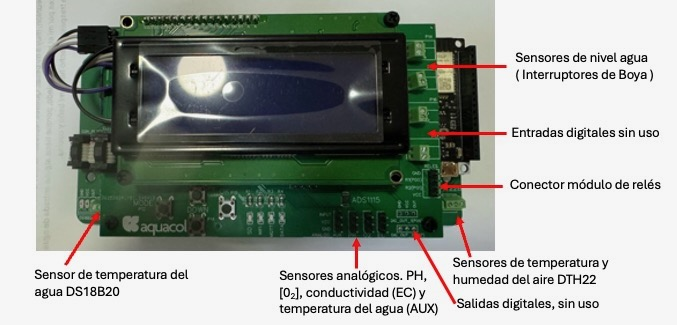
\psfig{file=Figuras/Montaje_Arriba.jpeg,width=16cm,angle=0}}
\caption{Placa montada Acuacol}\label{placa:acuacol}
\end{figure}

%%%%%%%%%%%%%%%%%%%%%%%%%%%%%%%%%%%%%%%%%%%%%
%                   relés                   %
%%%%%%%%%%%%%%%%%%%%%%%%%%%%%%%%%%%%%%%%%%%%%

En esta versión del Hardware de Acuacol \underline{no se usarán los sensores de nivel del agua ni el} \underline{módulo de relés}. Las conexiones están hechas de modo que cuando se crea conveniente puedan ser usadas. En la caja proporcionada deberían venir los módulos de relés.

\begin{figure}[htbp!]
\centering{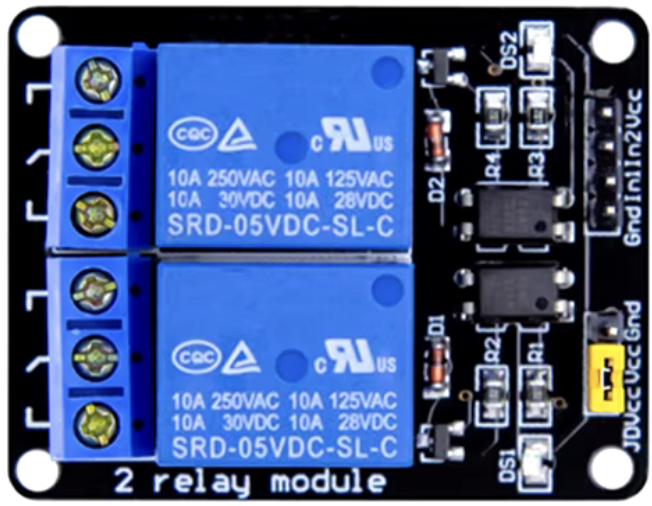
\psfig{file=Figuras/Modulo_reles.png,width=7cm,angle=0}}
\caption{Modulo de relés}\label{modulo:reles}
\end{figure}

Conexionado 
\begin{itemize}
\item El terminal \emph{GND} del módulo de relés se conecta al \emph{GND} del conector de relés de la placa.
\item El terminal \emph{VCC} del módulo de relés se conecta al \emph{VCC} del conector de relés de la placa.
\item El terminal \emph{IN1} del módulo de relés se conecta al \emph{R1(P00)} del conector de relés de la placa.
\item El terminal \emph{IN2} del módulo de relés se conecta al \emph{R2(P01)} del conector de relés de la placa.
\end{itemize}

P00 y P01 hacen referencia a la dirección de esos pines a nivel de programación.

%%%%%%%%%%%%%%%%%%%%%%%%%%%%%%%%%%%%%%%%%%%%%
%                   DTH22                   %
%%%%%%%%%%%%%%%%%%%%%%%%%%%%%%%%%%%%%%%%%%%%%

\subsection{Sensores de temperatura y humedad del aire DTH22}

Los sensores DTH22 no vienen conectados. Se conectan en la parte derecha de la placa inferior:

\begin{figure}[htbp!]
\centering{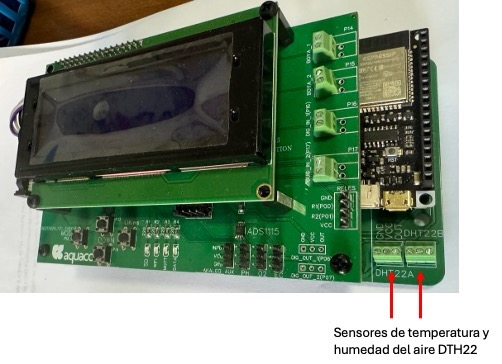
\psfig{file=Figuras/Montaje_derecha.jpeg,width=10cm,angle=0}}
\caption{Conexión en la placa del DTH22}\label{placa:acuacol:derecha}
\end{figure}

En la figura \ref{placa:acuacol:derecha} se pueden observar dos bornes para conectar dos sensores DTH22. La idea es que el sensor DTH22 conectado al borne "DTH22A" mida la temperatura y la humedad del aire en el interior de la sala donde se encuentran los depósitos de los peces. El sensor DTH22 conectado al borne "DTH22B" medirá la temperatura y la humedad del aire exterior. Para ello, este sensor debe instalarse en el exterior, asegurándose de que esté protegido del agua. Será necesario soldar un cable al sensor para esta instalación. El cable debe ser de al menos 3 hilos, apantallado, y no importa demasiado la sección del mismo. La longitud debe ser la mínima posible, ya que, aunque el protocolo de comunicaciones que utiliza el DTH22 permite cables bastante largos (20m según la literatura), el sensor funciona mejor con cables cortos.

\begin{figure}[htbp!]
\centering{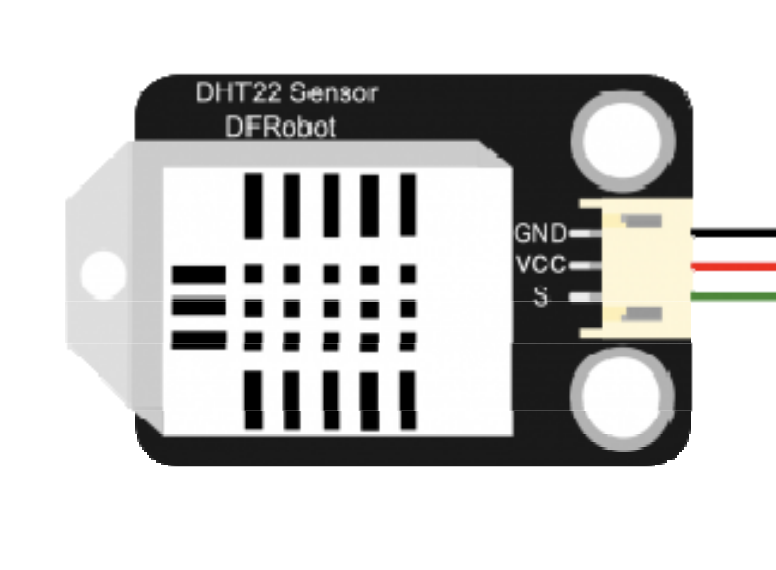
\psfig{file=Figuras/DTH22.png,width=10cm,angle=0}}
\caption{Conexion DTH22}\label{modulo:dth22}
\end{figure}

\begin{itemize}
\item El terminal \emph{GND} del DTH22 se conecta al \emph{GND} del borne "DTH22" de la placa.
\item El terminal \emph{VCC} del DTH22 se conecta al \emph{VCC} del borne "DTH22" de la placa.
\item El terminal \emph{S} del DTH22 se conecta al \emph{OUT} del borne "DTH22" de la placa.
\end{itemize}

Si la instalación es abierta, ambos sensores miden lo mismo. Solo se conectaría uno de los dos.

\begin{tcolorbox}
[colback=red!5!white,colframe=red!75!black,fonttitle=\bfseries,title=Desmontaje ]
Sea cuidadoso con el conexionado. Durante las pruebas del hardware se han pasado los tornillos con facilidad. Por eso, se recomienda el desmontaje de las placas para hacer las conexiones de forma más sencilla.
\begin{enumerate}
\item Quite los 4 tornillos de teflón del LCD (suelen ser solo 2). El LCD quedará unido a la placa de arriba por 4 hilos (figura \ref{desmontaje:1}).
\item Quite los 2 tornillos y los 2 separadores marcados en la figura \ref{desmontaje:2}. Quedará la placa de arriba suelta, conectada por un cable de 6 hilos a la placa inferior y por los 4 cables de los sensores analógicos. Puede quitar el conector de 6 hilos de la placa de arriba con la de abajo puesto que no tiene posibilidad de error al volverlo a montar. Puede quitarlos los cables de los sensores analógicos si tiene claro como van conectados. No quite los separadores de la parte inferior de la placa de arriba.
\item La placa inferior va unida a la caja con 2 tornillos metálicos (figura \ref{desmontaje:3}). Si los quita puede retirar la placa y hacer las conexiones cómodamente. Recuerde pasar los cables por el prensaestopa (pasacables) antes de hacer las conexiones. 
\item Para montar siga los pasos al contrario.
\end{enumerate}
\end{tcolorbox}

\begin{figure}[htbp!]
\centering{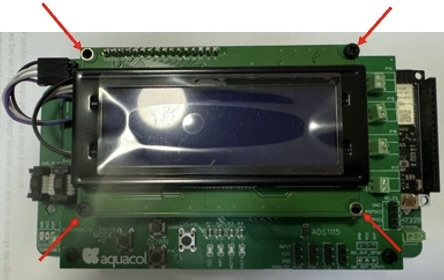
\psfig{file=Figuras/desmontaje1.jpeg,width=9cm,angle=0}}
\caption{Tornillos del modulo lcd.}\label{desmontaje:1}
\end{figure}

\begin{figure}[htbp!]
\centering{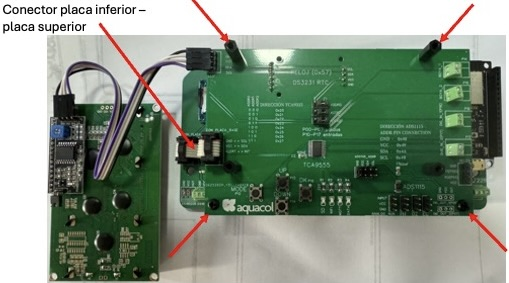
\psfig{file=Figuras/desmontaje2.jpeg,width=12cm,angle=0}}
\caption{Tornillos placa superior.}\label{desmontaje:2}
\end{figure}

\begin{figure}[htbp!]
\centering{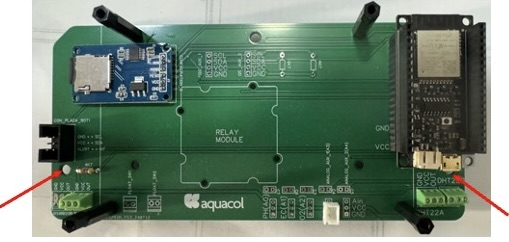
\psfig{file=Figuras/desmontaje3.jpeg,width=9cm,angle=0}}
\caption{Tornillos metálicos de placa inferior.}\label{desmontaje:3}
\end{figure}

%%%%%%%%%%%%%%%%%%%%%%%%%%%%%%%%%%%%%%%%%%%%%
%                   DS10B20                 %
%%%%%%%%%%%%%%%%%%%%%%%%%%%%%%%%%%%%%%%%%%%%%

\subsection{Sensor de temperatura del agua DS18B20}

El sensor DS1820 tampoco viene conectado. Se conectan en la parte izquierda de la placa inferior:

\begin{figure}[htbp!]
\centering{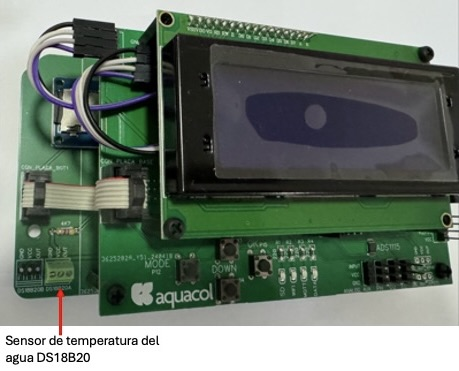
\psfig{file=Figuras/Montaje_DS18B20.jpg,width=10cm,angle=0}}
\caption{Conexión en la placa del DS18B20}\label{placa:acuacol:ds18b20}
\end{figure}

En la figura \ref{placa:acuacol:ds18b20} se observa que solo uno de los dos posibles bornes está soldado a la placa. Esto se debe a que, inicialmente, el equipo tenía dos sensores DS18B20, pero posteriormente se reemplazó uno de ellos por el sensor de temperatura incorporado en la sonda de conductividad. El objetivo es que este sensor mida la temperatura de un segundo tanque o piscina. Además, se utilizará esta sonda para calibrar el sensor de concentración de oxígeno ($O_2$) en caso de que se decida realizar la calibración con agua saturada. Esto se detallará en el apartado correspondiente (referencia pendiente).

\begin{figure}[htbp!] 
\centering{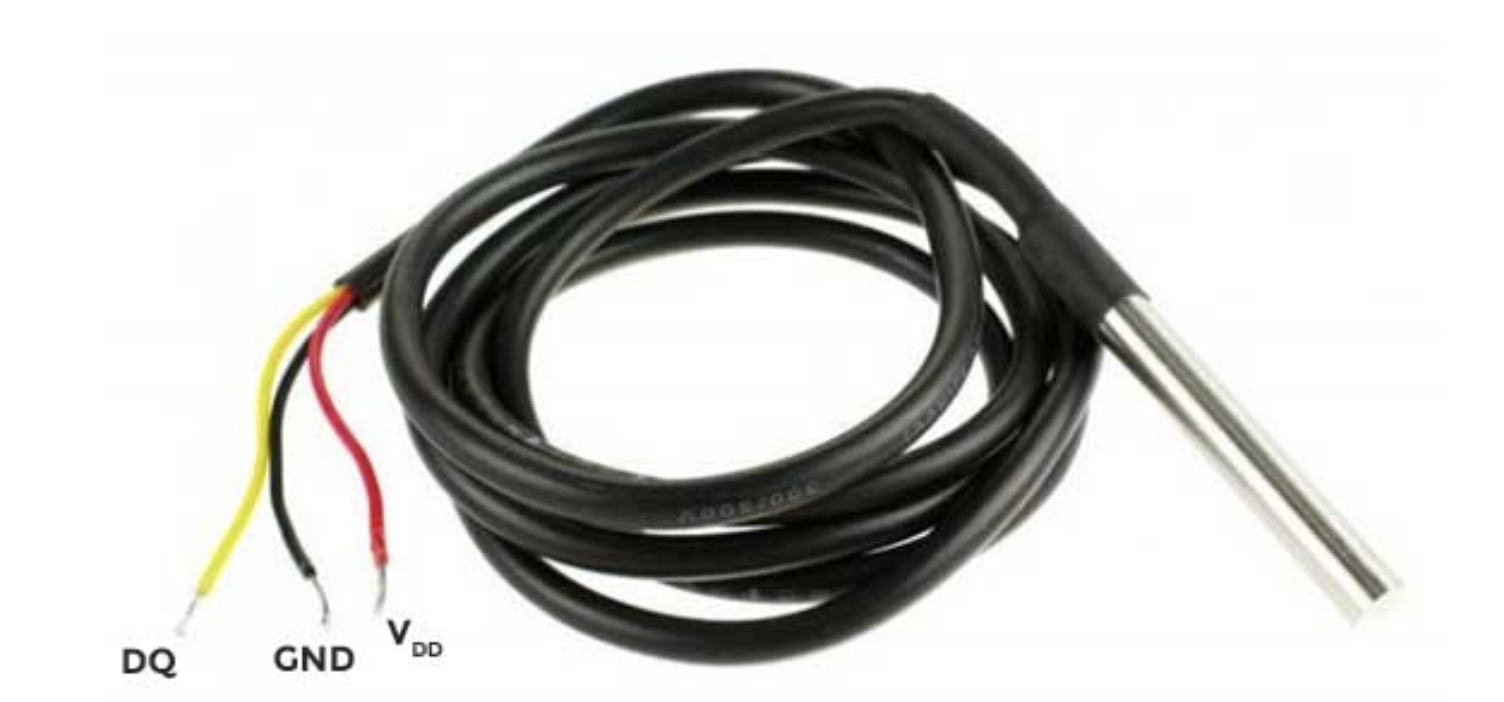
\psfig{file=Figuras/DS18B20.png,width=10cm,angle=0}} 
\caption{Sensor de temperatura del agua DS18B20}\label{sensor:ds18b20} 
\end{figure}

Las conexiones del DS18B20 se realizan de la siguiente manera:

\begin{itemize} 
\item El terminal \emph{GND} (negro) del DS18B20 se conecta al \emph{GND} del borne "DS18B20A" de la placa. 
\item El terminal \emph{VCC} (rojo) del DS18B20 se conecta al \emph{VCC} del borne "DS18B20A" de la placa. 
\item El terminal \emph{DQ} (amarillo) del DS18B20 se conecta al \emph{OUT} del borne "DS18B20A" de la placa. 
\end{itemize}

Se recomienda utilizar el propio cable que trae la sonda. Si el cable es demasiado corto, se puede extender con un cable de 3 hilos apantallado, similar al que trae el sensor. Es preferible mantener el cable lo más corto posible. Aunque la literatura indica que el protocolo 1-Wire, que utiliza el DS18B20, admite longitudes de cable de hasta 200 metros, algunos autores sugieren no exceder los 8 metros. Para evitar la corrupción de la señal, se ha añadido una resistencia PULLUP de 4.7 $k\Omega$.

\subsection{Sensores analógicos}

Los sensores analógicos son aquellos que me dan la medida en forma de tensión. Son muy sensibles a interferencias y se deben poner lo más cerca posible del equipo. Como todos estos sensores se ponen juntos en el baño donde se hallen los peces , el equipo habría de situarse lo más cerca posible de este baño.

Estos sensores son:
\begin{itemize}
\item \textbf{Sensor de PH DFRobot SEN0169-V2}. El transductor (la placa que adapta la señal de la sonda para que pueda ser leída por el microcontrolador) del sensor de pH ya viene conectado, por lo que solo es necesario conectar la sonda de pH al conector en el exterior del equipo.  
\begin{figure}[htbp!] 
\centering{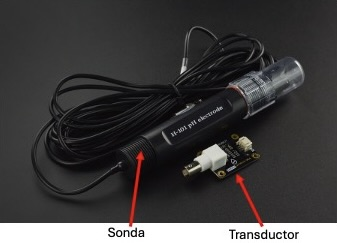
\psfig{file=Figuras/PH.jpg,width=10cm,angle=0}} 
\caption{Sensor de PH DFRobot SEN0169-V2}\label{sensor:PH} 
\end{figure}
Se puede observar que el transductor del sensor de pH está unido a otra placa, la DFRobot DFR0504, que es un aislador analógico (ANALOG ISOLATOR) (figura \ref{sensor:iso}). Este aislador se utiliza para evitar el acoplamiento entre las diferentes señales analógicas a través del agua.
\begin{figure}[htbp!] 
\centering{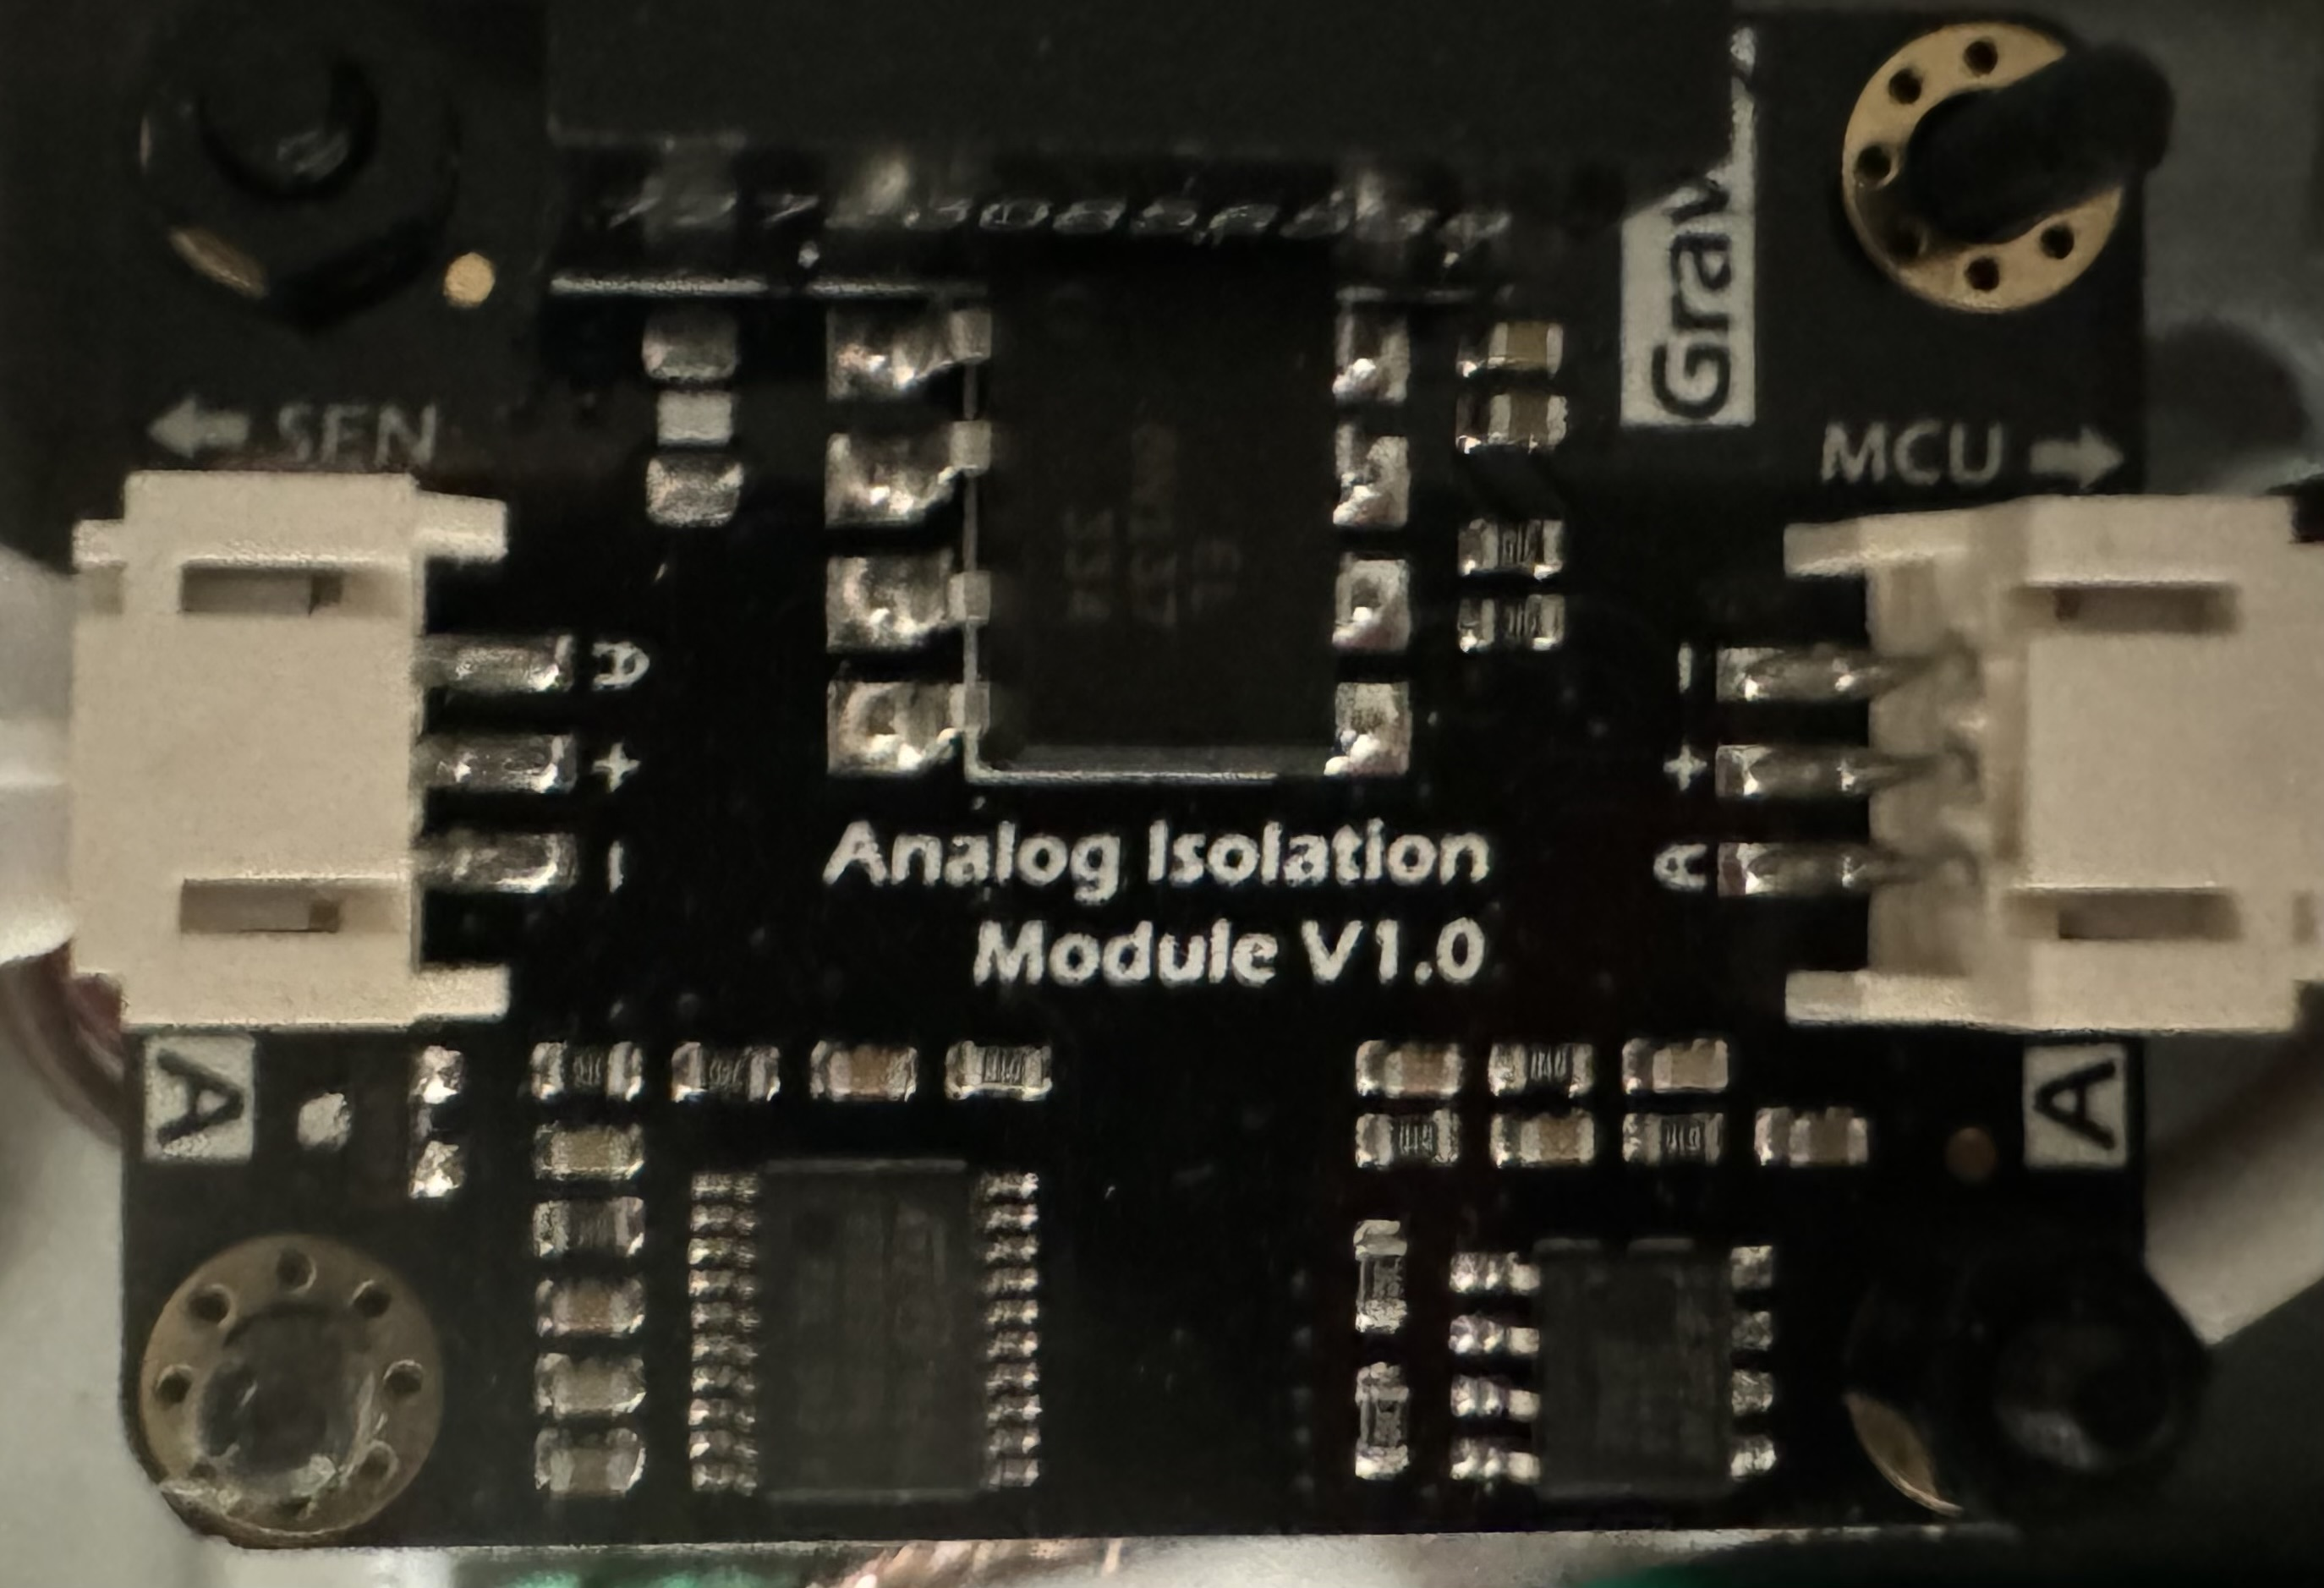
\psfig{file=Figuras/Analog_isolator.jpeg,width=8cm,angle=0}} 
\caption{Analog isolator}\label{sensor:iso} 
\end{figure}

Lo mismo ocurre con los transductores del sensor de 02 y del de conductividad.

\item \textbf{El sensor de concentración de oxígeno DFRobot SEN0237-A}. El transductor ya está conectado, solo hay que poner la sonda de $O_2$ en el conector en el exterior del equipo. 
\begin{figure}[htbp!] 
\centering{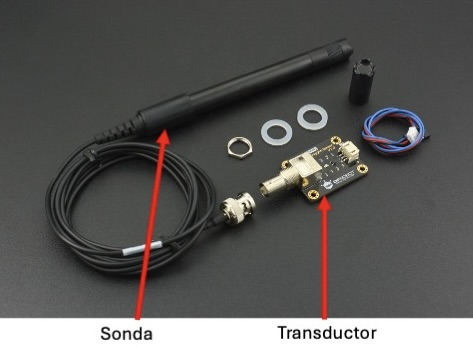
\psfig{file=Figuras/O2.jpg,width=10cm,angle=0}} 
\caption{Sensor de O2 DFRobot SEN0237-A}\label{sensor:O2} 
\end{figure}

\item El sensor de conductividad y temperatura (DFRobot SEN0451). los transductores (las placas que adaptan las señales de la sonda para que las pueda leer el micro) vienen apilados uno sobre otro en la parte inferior izquierda de la caja ya vienen conectados. Se puede observar que vienen sueltos, es porque hay que poner los conectores correspondientes a la sonda de conductividad y temperatura (figura \ref{sensor:EC}, Conector transductor -sensor). Estos conectores no entran por el agujero del prensaestopa (pasacables) negro que está atornillado en la parte inferior de la caja. 
\begin{figure}[htbp!] 
\centering{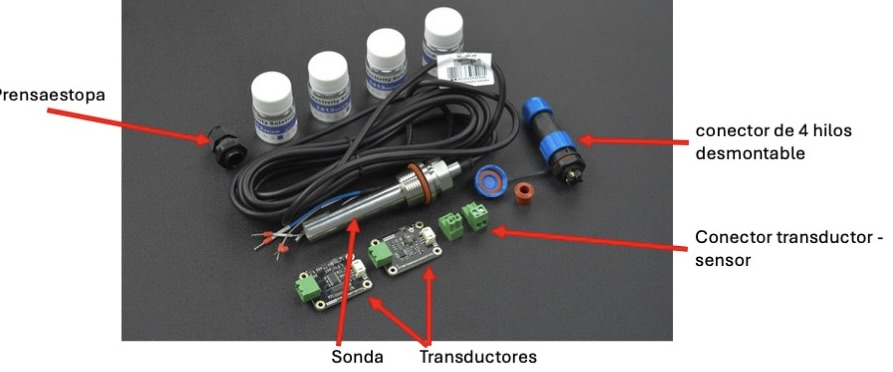
\psfig{file=Figuras/EC.jpg,width=14cm,angle=0}} 
\caption{Sensor de EC DFRobot SEN0451}\label{sensor:EC} 
\end{figure}

Por lo que se procederá de la siguiente manera:
\begin{enumerate}
\item Pasamos el cable (figura \ref{sensor:CEC}) de la sonda por el prensaestopa de color negro (que ya está puesto en la caja).
\item Conectamos los cables a los conectores transductor-sensor (ver figura \ref{sensor:EC}). En una de las fichas verdes se conectan los dos cables marcados con \emph{temp} (figura \ref{sensor:CEC}). No importa el orden (figura \ref{sensor:temp}).\\ 
\begin{figure}[htbp!] 
\centering{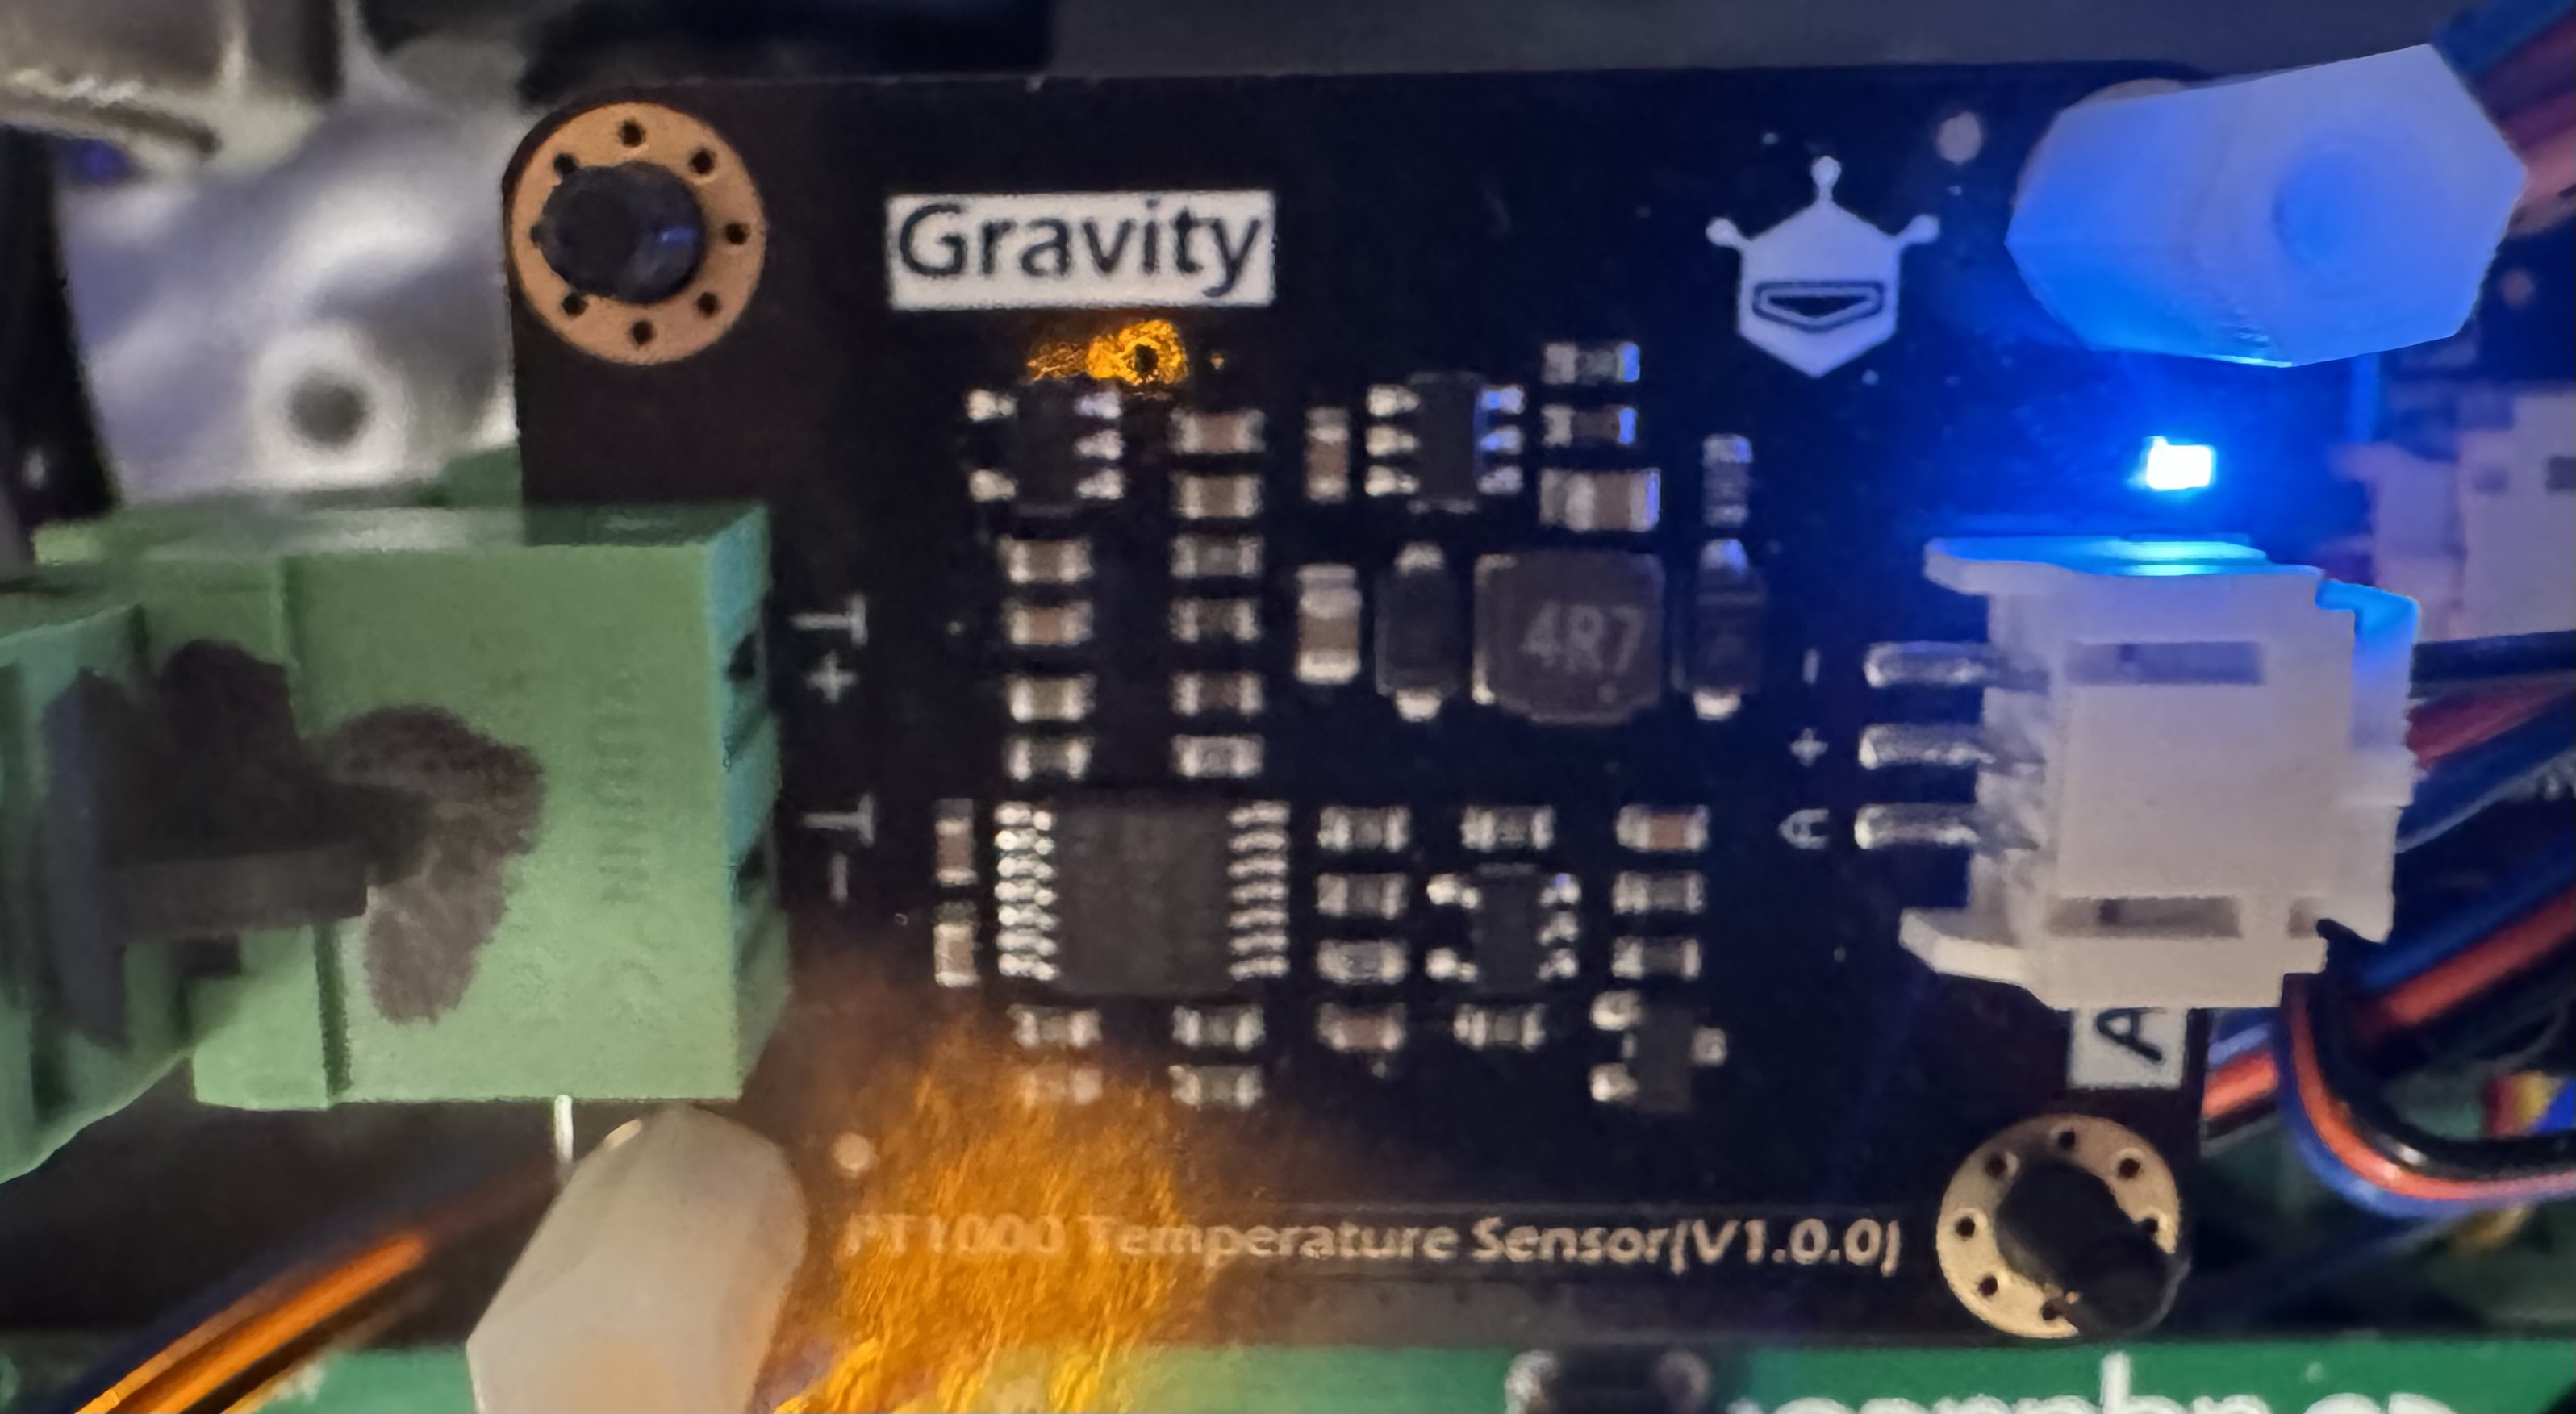
\psfig{file=Figuras/Temperature_transductor.jpeg,width=8cm,angle=0}} 
\caption{Transductor de temperatura del sensor de conductividad}\label{sensor:temp} 
\end{figure}
Los dos cables restantes, $S-$ y $S+$ (En nuestra sonda el cable S+ es tan fino que no lleva etiqueta) se conectan en la otra ficha verde, pero este sensor, el de conductividad, si tiene polaridad. De los dos transductores, que están apilados a la izquierda abajo de la caja, el superior es el correspondiente a la conductividad, (lo pone en la placa). Si se observa en el conector hembra de la ficha verde se puede ver que terminal es el positivo y cual el negativo. 
\begin{figure}[htbp!] 
\centering{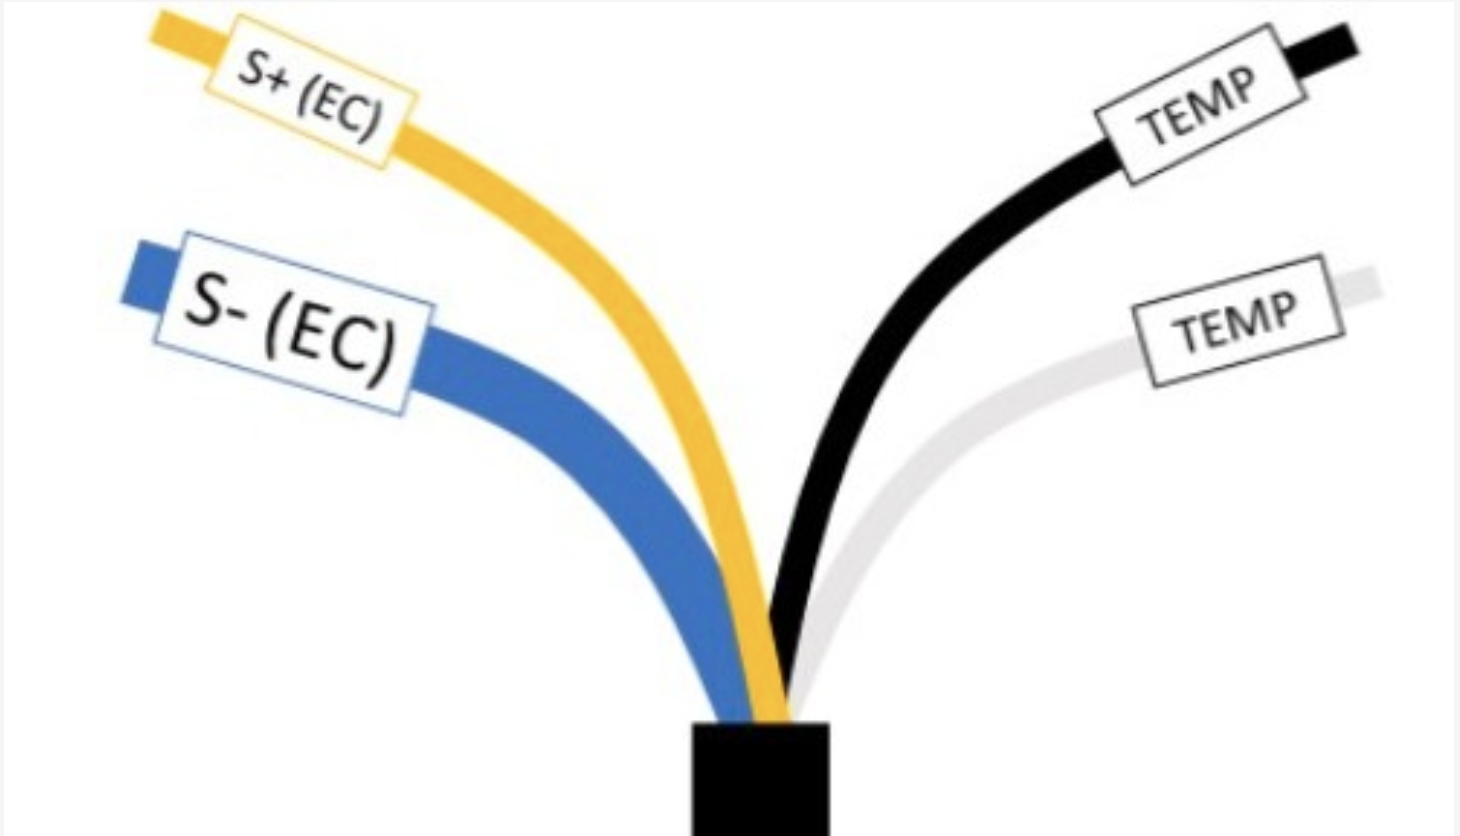
\psfig{file=Figuras/Cables_EC.png,width=6cm,angle=0}} 
\caption{Cables sonda sensor EC}\label{sensor:CEC} 
\end{figure}
\item Conectamos en el transductor superior la ficha verde correspondiente al sensor de conductividad y en la inferior en de la temperatura. Hay una tercera plaquita en el apilamiento que es otro ANALOG ISOLATOR.
\item Sacamos el cable que podamos por el prensaestopa y lo apretamos para que quede estanco.
\end{enumerate}

\end{itemize}

Los transductores de cada sensor van conectados a la placa de arriba en el lugar correspondiente:
\begin{figure}[htbp!] 
\centering{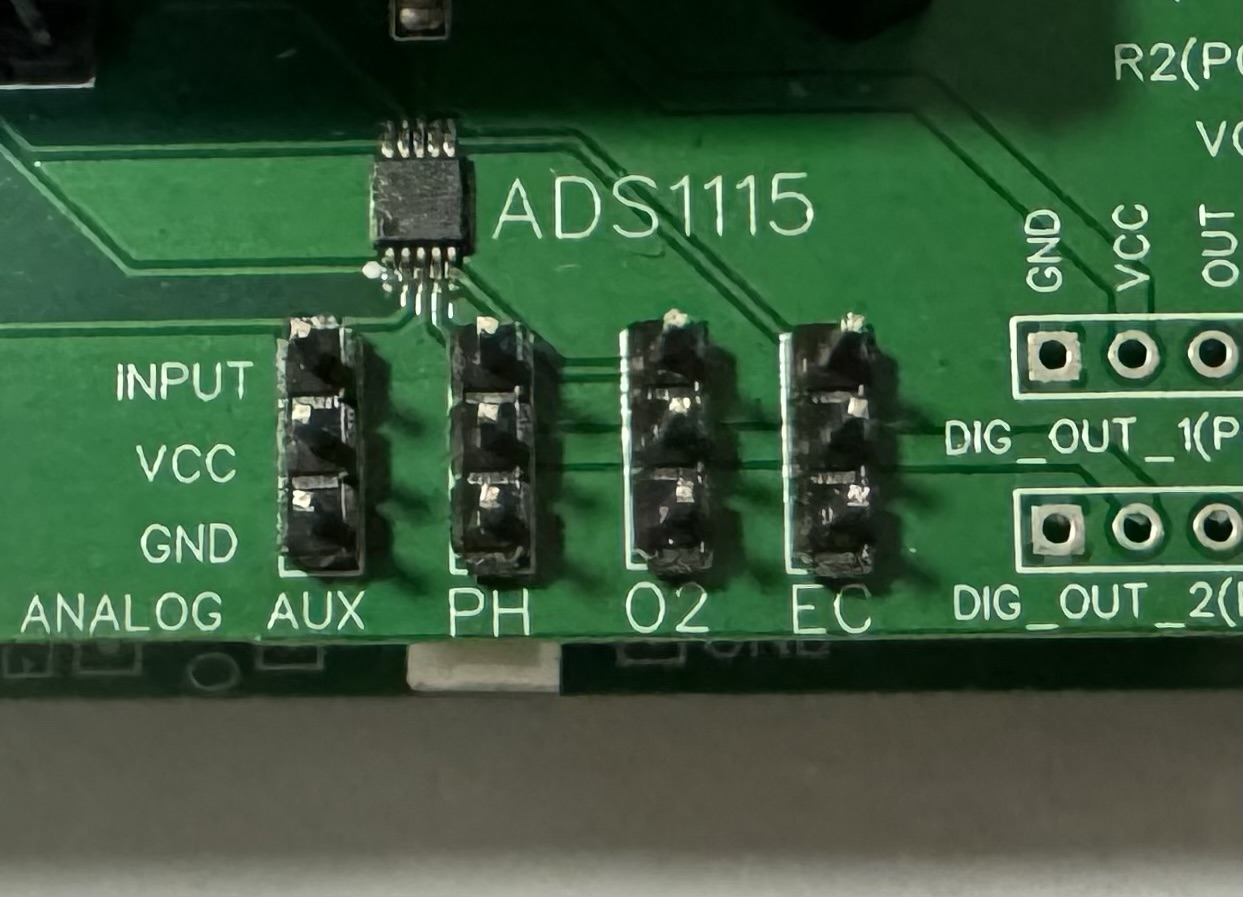
\psfig{file=Figuras/entradas_analogicas.jpeg,width=10cm,angle=0}} 
\caption{Bornes entradas analógicas}\label{sensor:Anal} 
\end{figure}
\begin{itemize}
\item El sensor de PH va conectado a los 3 pines marcados con PH. 
\item El sensor de Concentración de $O_2$ va conectado a los 3 pines marcados con O2. 
\item El sensor de Conductividad va conectado a los 3 pines marcados con EC.
\item El sensor de temperatura del la sonda de conductividad va conectado a los 3 pines marcados con AUX.
\end{itemize}

Los cables que vienen de los transductores, están compuesto por 3 hilos de los cuales uno es \underline{negro y va conectado a GND.}

\section{Puesta en marcha}

Hay que que hablar de la tarjeta micro SD y del archivo \emph{config.txt}

\begin{verbatim}
{"ssid":"MiFibra-8980","password":"nmH9Rxkt","PH1":7.3,"mV1":1715,"PH2":9.8,
"mV2":1218,"CAL1_V":256,"CAL1_T":25.75,"CAL2_V":1507,"CAL2_T":18.4,"Kec":0.9569,
"Tec":25,"mS":1413,"id":3}
\end{verbatim}

Este fichero contiene los datos de la red y los parámetros de configuración de los sensores analógicos. Veamoslo campo por campo:
\begin{itemize}
\item \textbf{"ssid":"MiFibra-8980"}. Tendrá que sustituir \emph{MiFibra-8980} por el nombre de su WIFI. Tenga en cuenta que el esp32, el micro que lleva el equipo, tiene una antena muy pequeña por lo que necesitará una señal fuerte para poder transmitir sin problemas.
\item \textbf{"password":"nmH9Rxkt"}. Tendrá que sustituir \emph{nmH9Rxkt} por el password de su WIFI.
\item \textbf{"PH1":7.3,"mV1":1715,"PH2":9.8,"mV2":1218}. Son los parámetros de configuración del sensor de PH. No los modifique, se modificarán de forma automática cuando configure dicho sensor.
\item \textbf{"\ CAL1\_V":256,"\ CAL1\_T":25.75,"\ CAL2\_V":1507,"\ CAL2\_T":18.4}. Son los parámetros de configuración del sensor de concentración de $O_2$. No los modifique, se modificarán de forma automática cuando configure dicho sensor.
\item \textbf{"Kec":0.9569,"Tec":25,"mS":1413}. Son los parámetros de configuración del sensor de concentración de Conductividad. \underline{Modifique únicamente el valor de Kec} con el valor que viene pegado en el cable de las sonda de conductividad (que es la calibración inicial, figura \ref{sensor:Kec}). Cuando pase el tiempo y el sensor necesite ser recalibrado los parámetros se modificarán de forma automática cuando configure dicho sensor.
\begin{figure}[htbp!] 
\centering{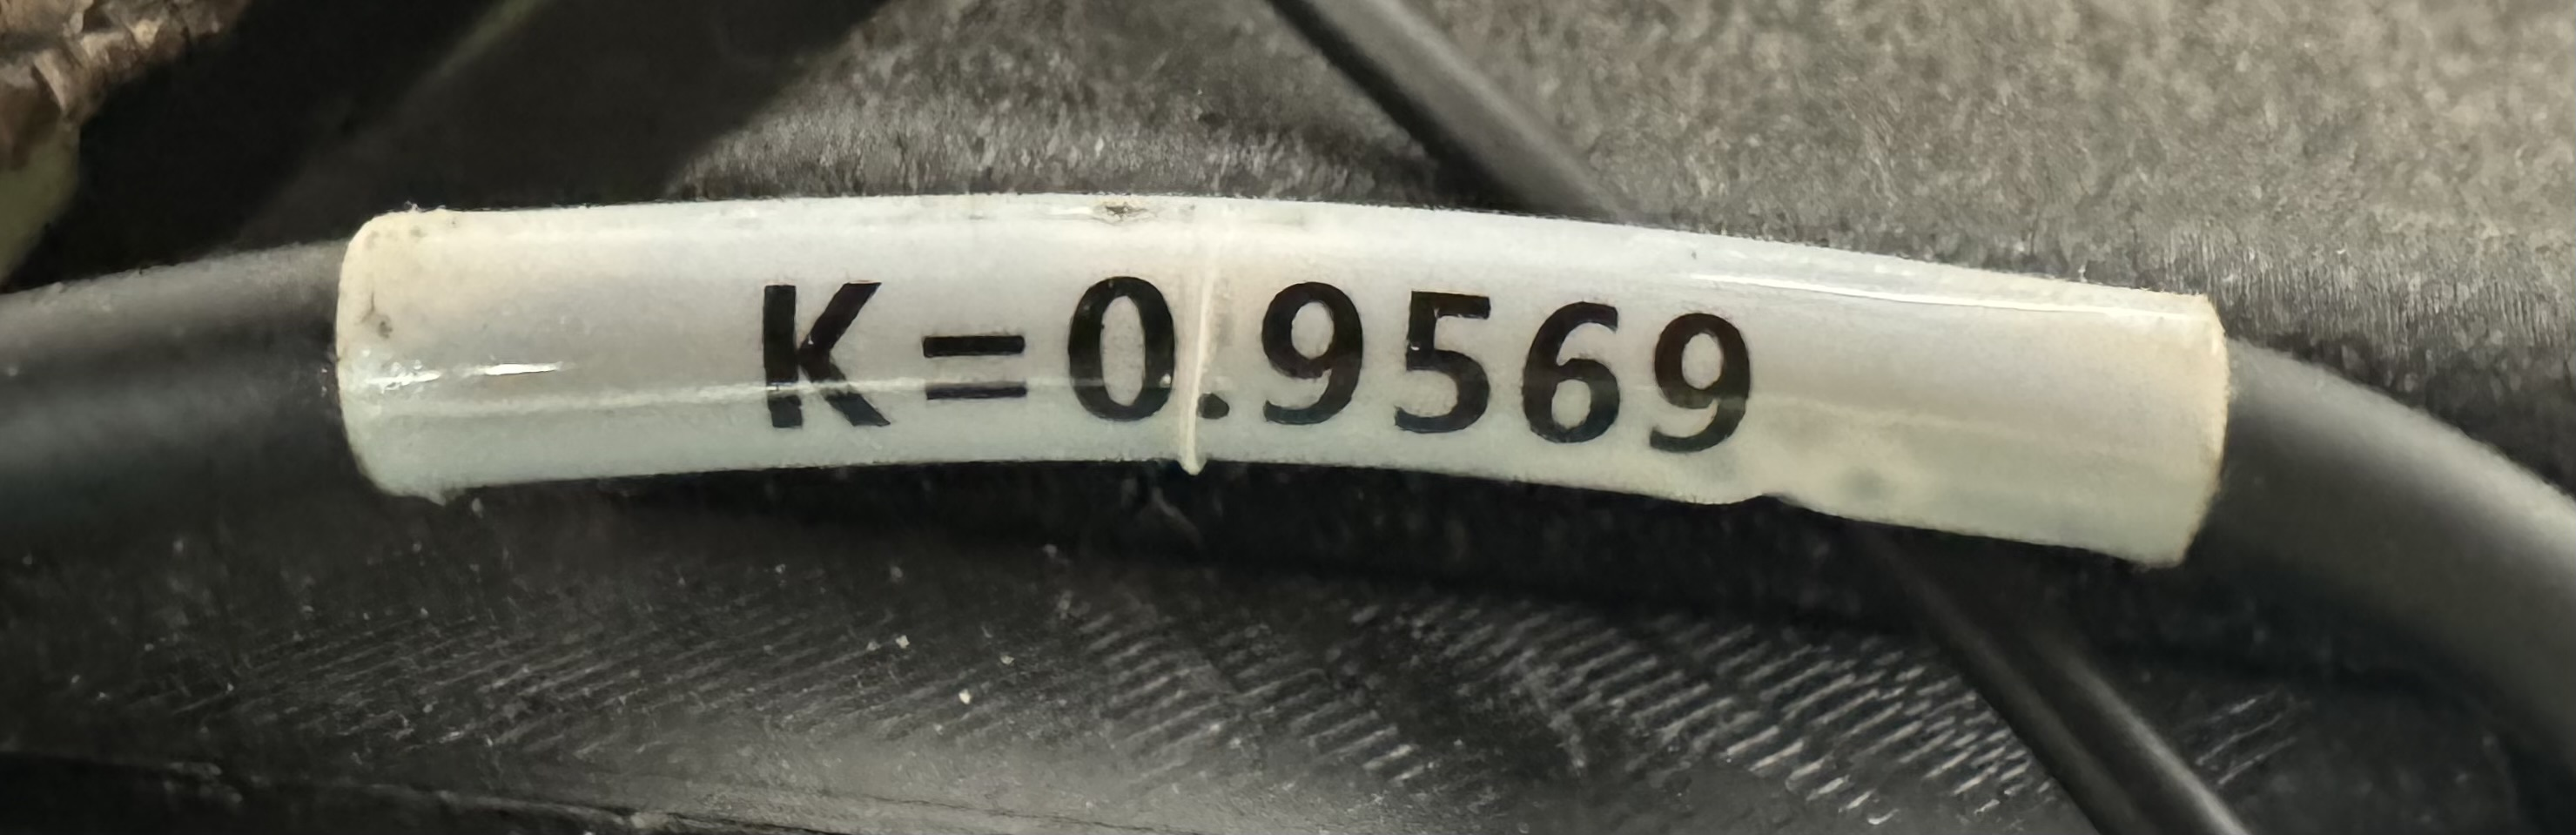
\psfig{file=Figuras/Kec.jpeg,width=6cm,angle=0}} 
\caption{Valor inicial de Kec}\label{sensor:Kec} 
\end{figure}
\item \textbf{"\ id":3}. Cada equipo tiene su propio \emph{id}. Este número determinará a que base de datos se mandan los datos recogidos. Víctor debería tener esa información.
\end{itemize}

Una vez actualizada la información , puede volver a introducir la tarjeta y en la secuencia de arranque del equipo, podría ver:
\begin{enumerate}
\item Que detecta la tarjeta microSD (se enciende el primer led de la placa superior). Si no lo hace pruebe a sacar y volver a poner la tarjeta. (Puede ver los leds en la figura \ref{botones}).
\item Que se conecta a internet, (se enciende el segundo led de la placa superior). Si no se conecta es porque no se ha puesto el nombre y la contraseña de forma correcta o porque la señal es muy débil. Pruebe a crear un punto de acceso con un móvil cerca. Configure la red en la tarjeta SD y si se conecta es por eso, tendrá que pensar como poner el router más cerca del dispositivo.
\item Una vez tenga wifi la hora del reloj se actualizará de forma automática. También se actualizará la hora del módulo de reloj interno. Este módulo mantienen la hora incluso cuando haya cortes de corriente y el aparato arranque sin covertura WIFI. Pero al menos la primera vez debe tener cobertura WIFI para que pueda actualizar la misma. Si alguna vez se perdiera la hora después de un corte de corriente , seguramente es porque se ha gastado la pila del módulo de reloj que está debajo de la placa superior del equipo. 
\item Se conecta al servidor mqtt. (se enciende el tercer led de la placa superior). Si no se conecta pero si se ha conectado a la wifi el problema debe estar en los servidores de la base de datos.
\item El cuarto led se encenderá cuando mande un dato 15 min después de que se encienda. Si durante su funcionamiento se apagase , es que no ha podido mandar el último dato. Siempre quedará una copia del mismo en la tarjeta microSD y en versiones futuras del programa se enviarán los datos que no se hallan podido mandar cuando vuelva a haber cobertura wifi.
\end{enumerate}


\clearpage

\chapter{Calibración de los sensores}
%%%%%%%%%%%%%%%%%%%%%%%%%%%%%%%%%%%%%%%%%%%%%%%%%%%%%%%%%%%%%%%%%%%%%%%%%%%%%%%%%%%%%%%%%%%%%%%%%%%%%%

Con objeto de facilitar la configuración de los sensores analógicos, se han habilitado 4 botones al equipo.

\begin{figure}[htbp!] 
\centering{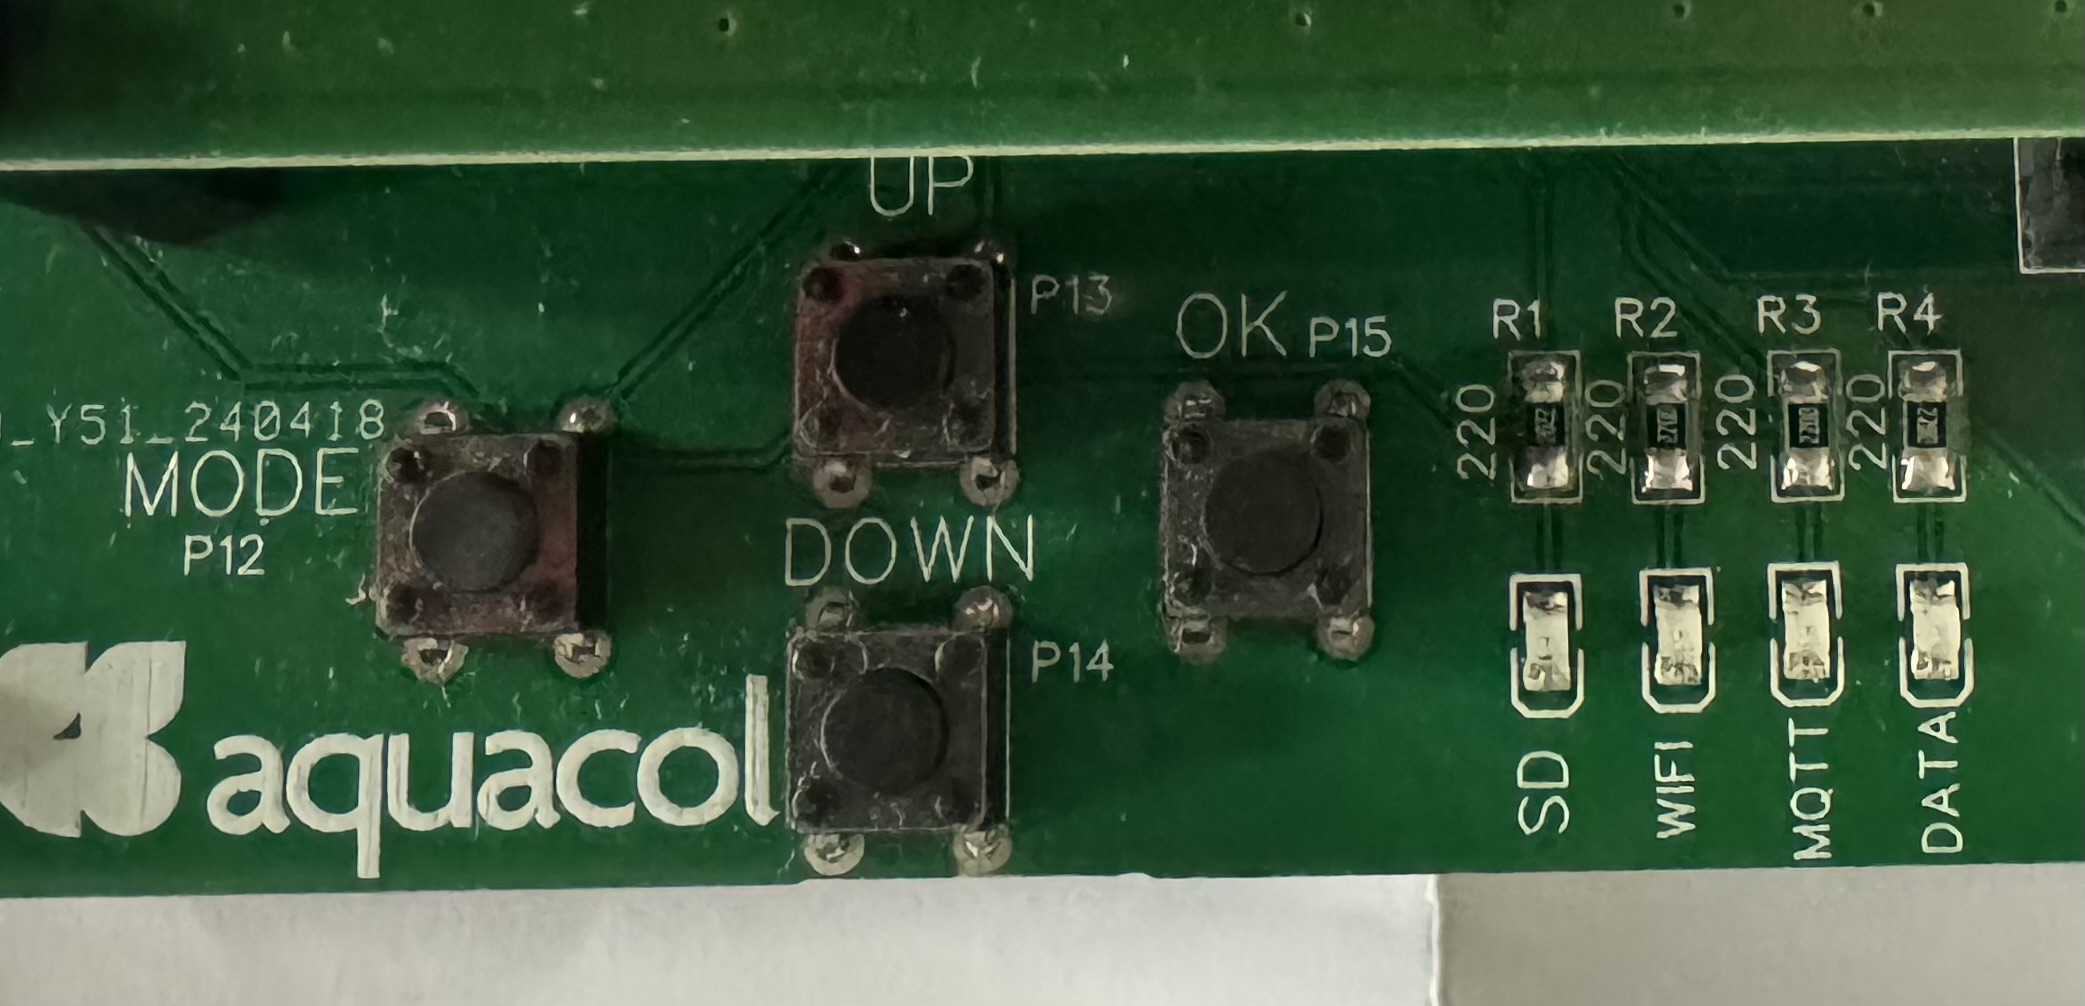
\psfig{file=Figuras/Botones.jpeg,width=10cm,angle=0}} 
\caption{Botones y leds de estado}\label{botones} 
\end{figure}

Puede ver que hay 4 botones
\begin{itemize}
\item \textbf{MODE}. Nos sirve para cambiar de pantalla.
\item \textbf{UP}. Nos sirve para subir determinado parámetro en la calibración. Va a depender de la pantalla en la que se esté.
\item \textbf{DOWN}. Nos sirve para bajar determinado parámetro en la calibración. Va a depender de la pantalla en la que se esté.
\item \textbf{OK}. Guardará la configuración de del parámetro en el archivo \emph{config.txt} y volverá a la pantalla por defecto.
\end{itemize}

Los botones puede parecer que a veces no funcionan, es normal. Es debido a un problema de rebotes (falsos contactos) se está trabajando en solucionarlo. No se pulsan solos , solo a veces no detecta que se pulsan.

\section{Secuencia de arranque}

Cuando arranca el equipo pasa por una serie de pantallas:
\begin{enumerate}
\item Primero configura la tarjeta microSD, es importante que esta parte funcione porque en la tarjeta está toda la información de la WIFI y de configuración de los sensores. Se encenderá el led con la etiqueta SD de la figura \ref{botones}.

En caso de que la tarjeta microSD no esté bien configurada (ver figura \ref{patalla:Nosd}), ya sea porque el formato no es el correcto (FAT 32), porque no está bien pinchada en el alojamiento o porque no exista en la tarjeta el archivo \emph{config.txt}. 

\begin{figure}[htbp!] 
\centering{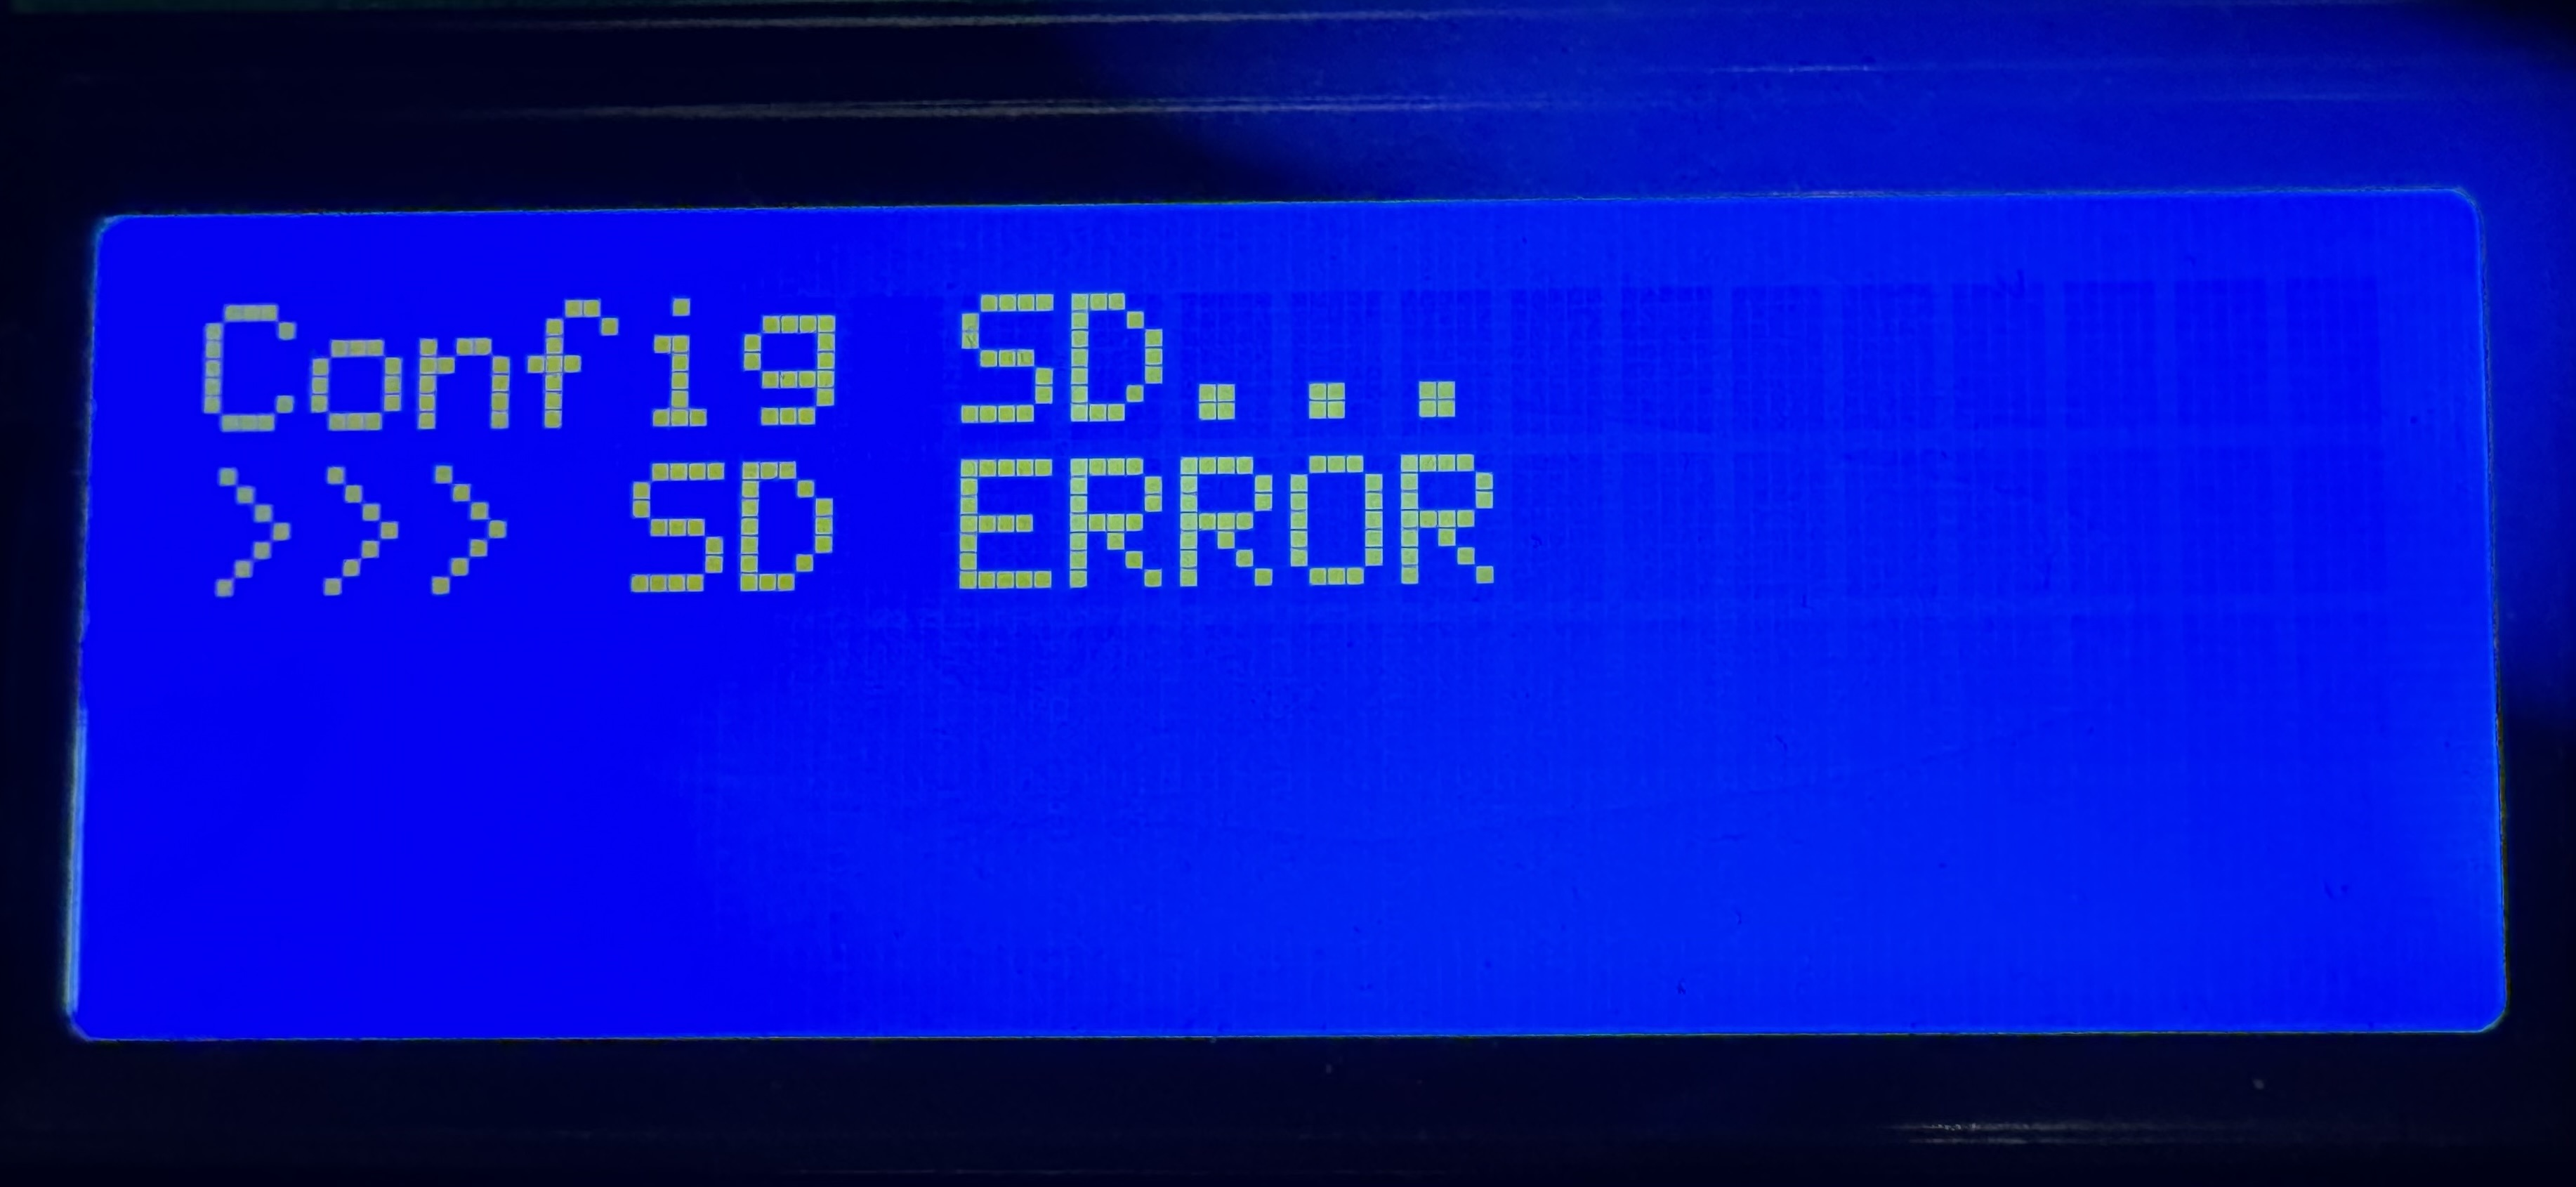
\psfig{file=Figuras/SD_ERROR.jpeg,width=8cm,angle=0}} 
\caption{SD ERROR}\label{patalla:Nosd} 
\end{figure}

Se cargará la configuración por defecto (figura \ref{patalla:condef} )  

\begin{figure}[htbp!] 
\centering{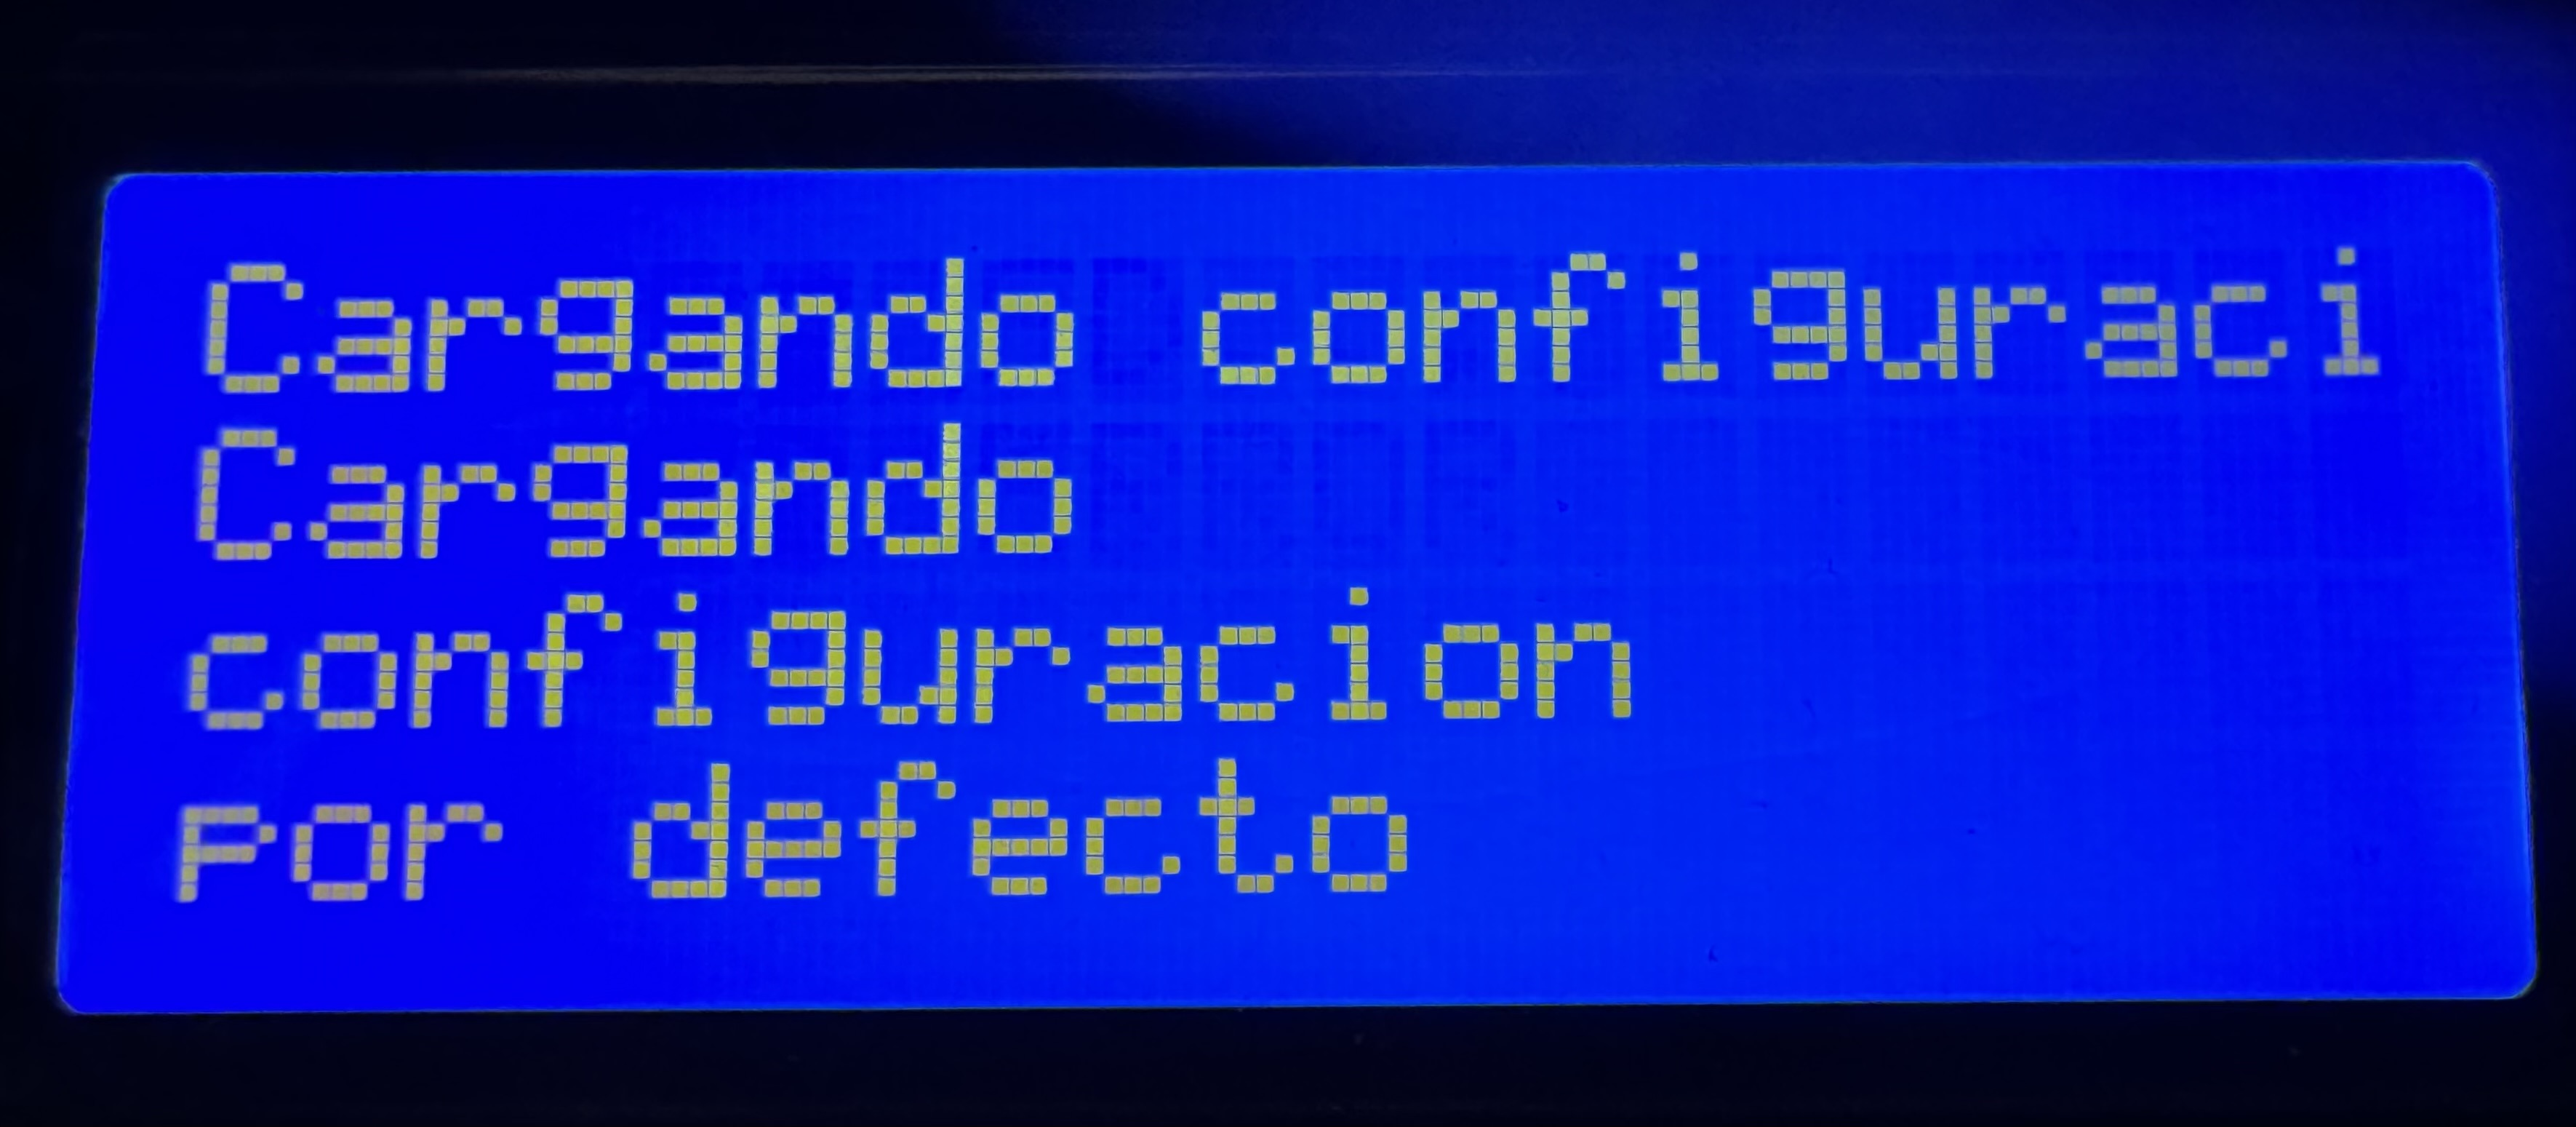
\psfig{file=Figuras/Conf_def.jpeg,width=8cm,angle=0}} 
\caption{Cargada configuración por defecto}\label{patalla:condef} 
\end{figure}

Que es la configuración aquí en Sevilla.

Puede ser interesante continuar si no existe el fichero \emph{config.txt}, porque al guardar cualquier configuración de cualquier sensor se creará el archivo en al tarjeta y podremos editarlo para poner la configuración WIFI a posteriori.

%%%%%%%%%%%%%%%%%%%%%%%%%%%%%%%%%%%%%%%%%%%%%%%%%%%%%%%%%%%%%%%%%%%%%%%%%%%%%%%%%%%%%%%%%%%%%

\item En caso de que la tarjeta microSd esté bien configurada (figura \ref{patalla:sd}). 

\begin{figure}[htbp!] 
\centering{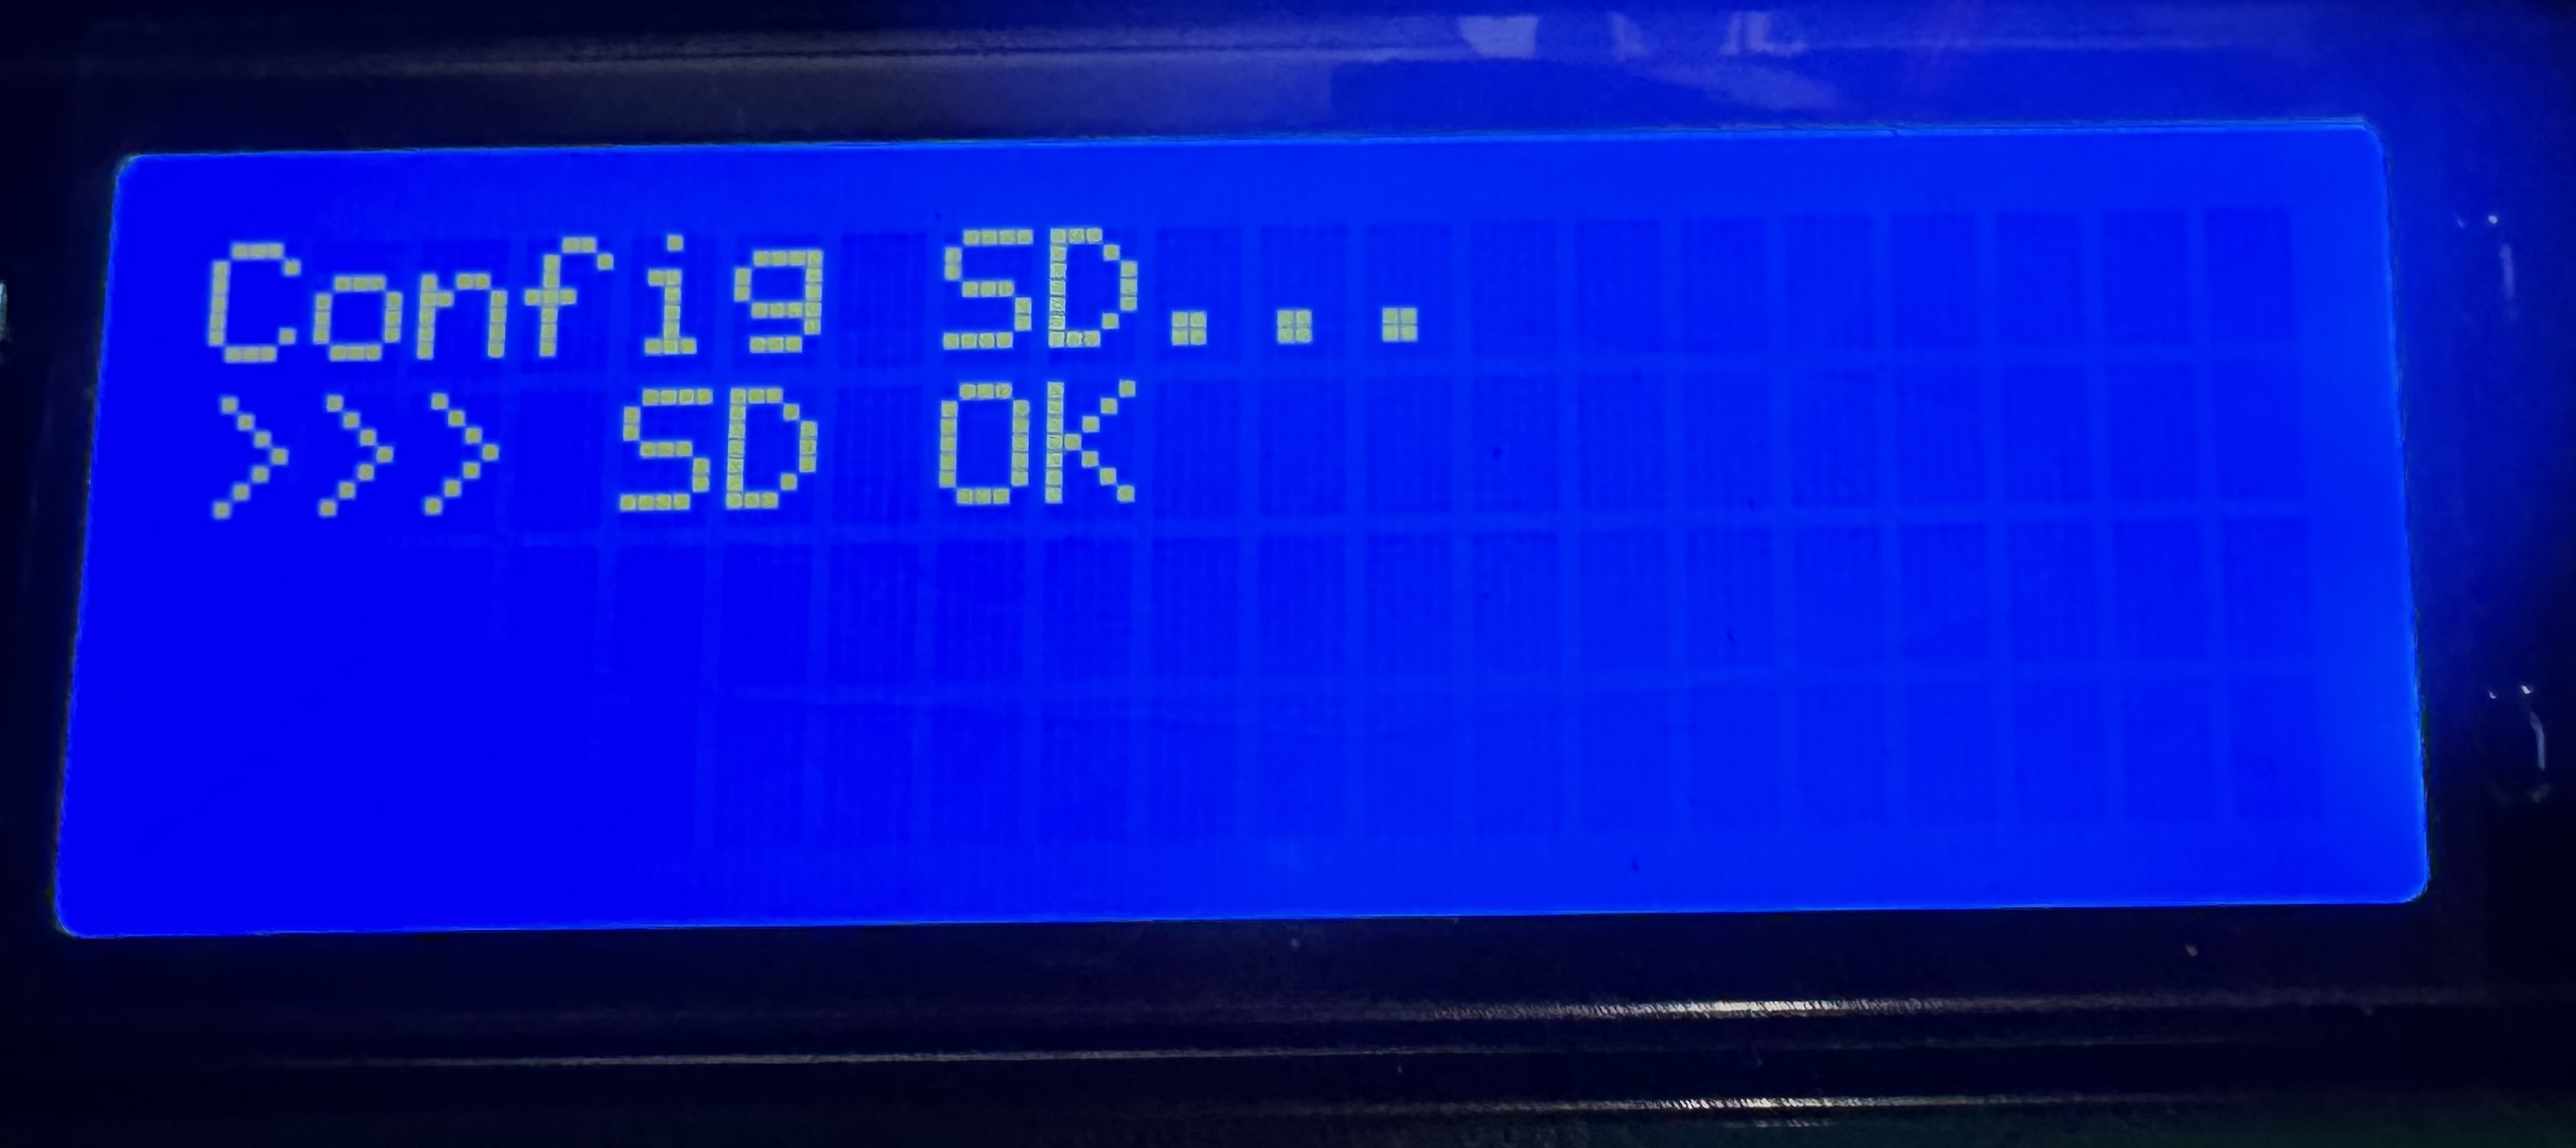
\psfig{file=Figuras/SD_OK.jpeg,width=8cm,angle=0}} 
\caption{SD OK}\label{patalla:sd} 
\end{figure}

Carga la configuración de los sensores (figura \ref{patalla:SenOk}).

\begin{figure}[htbp!] 
\centering{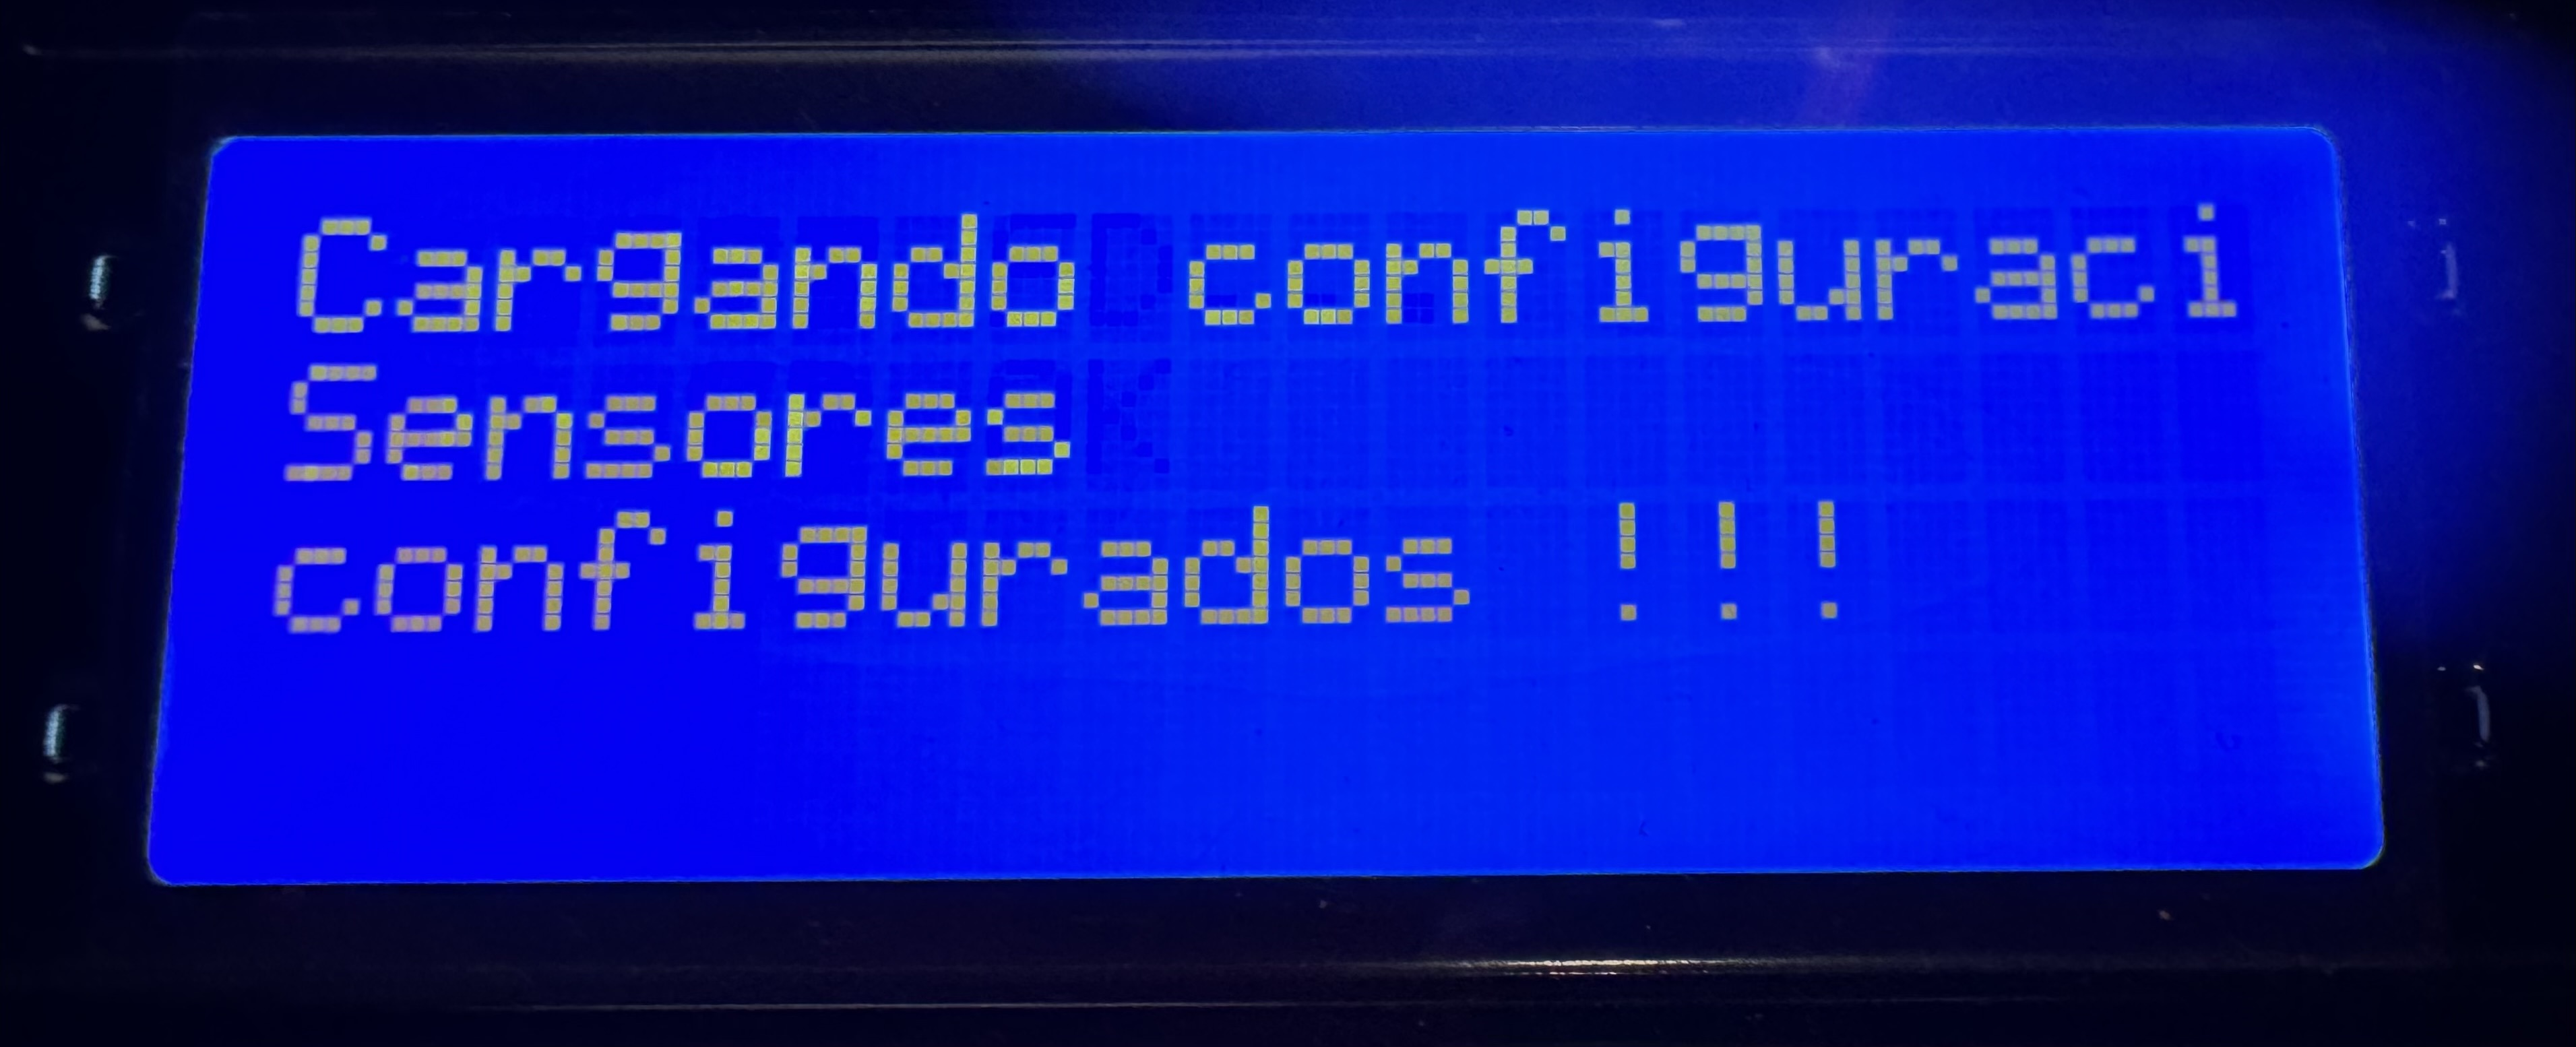
\psfig{file=Figuras/sensores_OK.jpeg,width=8cm,angle=0}} 
\caption{Cargada la configuración de los sensores}\label{patalla:SenOk} 
\end{figure}

%%%%%%%%%%%%%%%%%%%%%%%%%%%%%%%%%%%%%%%%%%%%%%%%%%%%%%%%%%%%%%%%%%%%%%%%%%%%%%%%%%%%%%%%%%%%%%%%
\newpage
\item Después configura la WIFI. Lo intentará 5 veces y si con ninguna de los 5 lo consigue aparecerá por pantalla:

\begin{figure}[htbp!] 
\centering{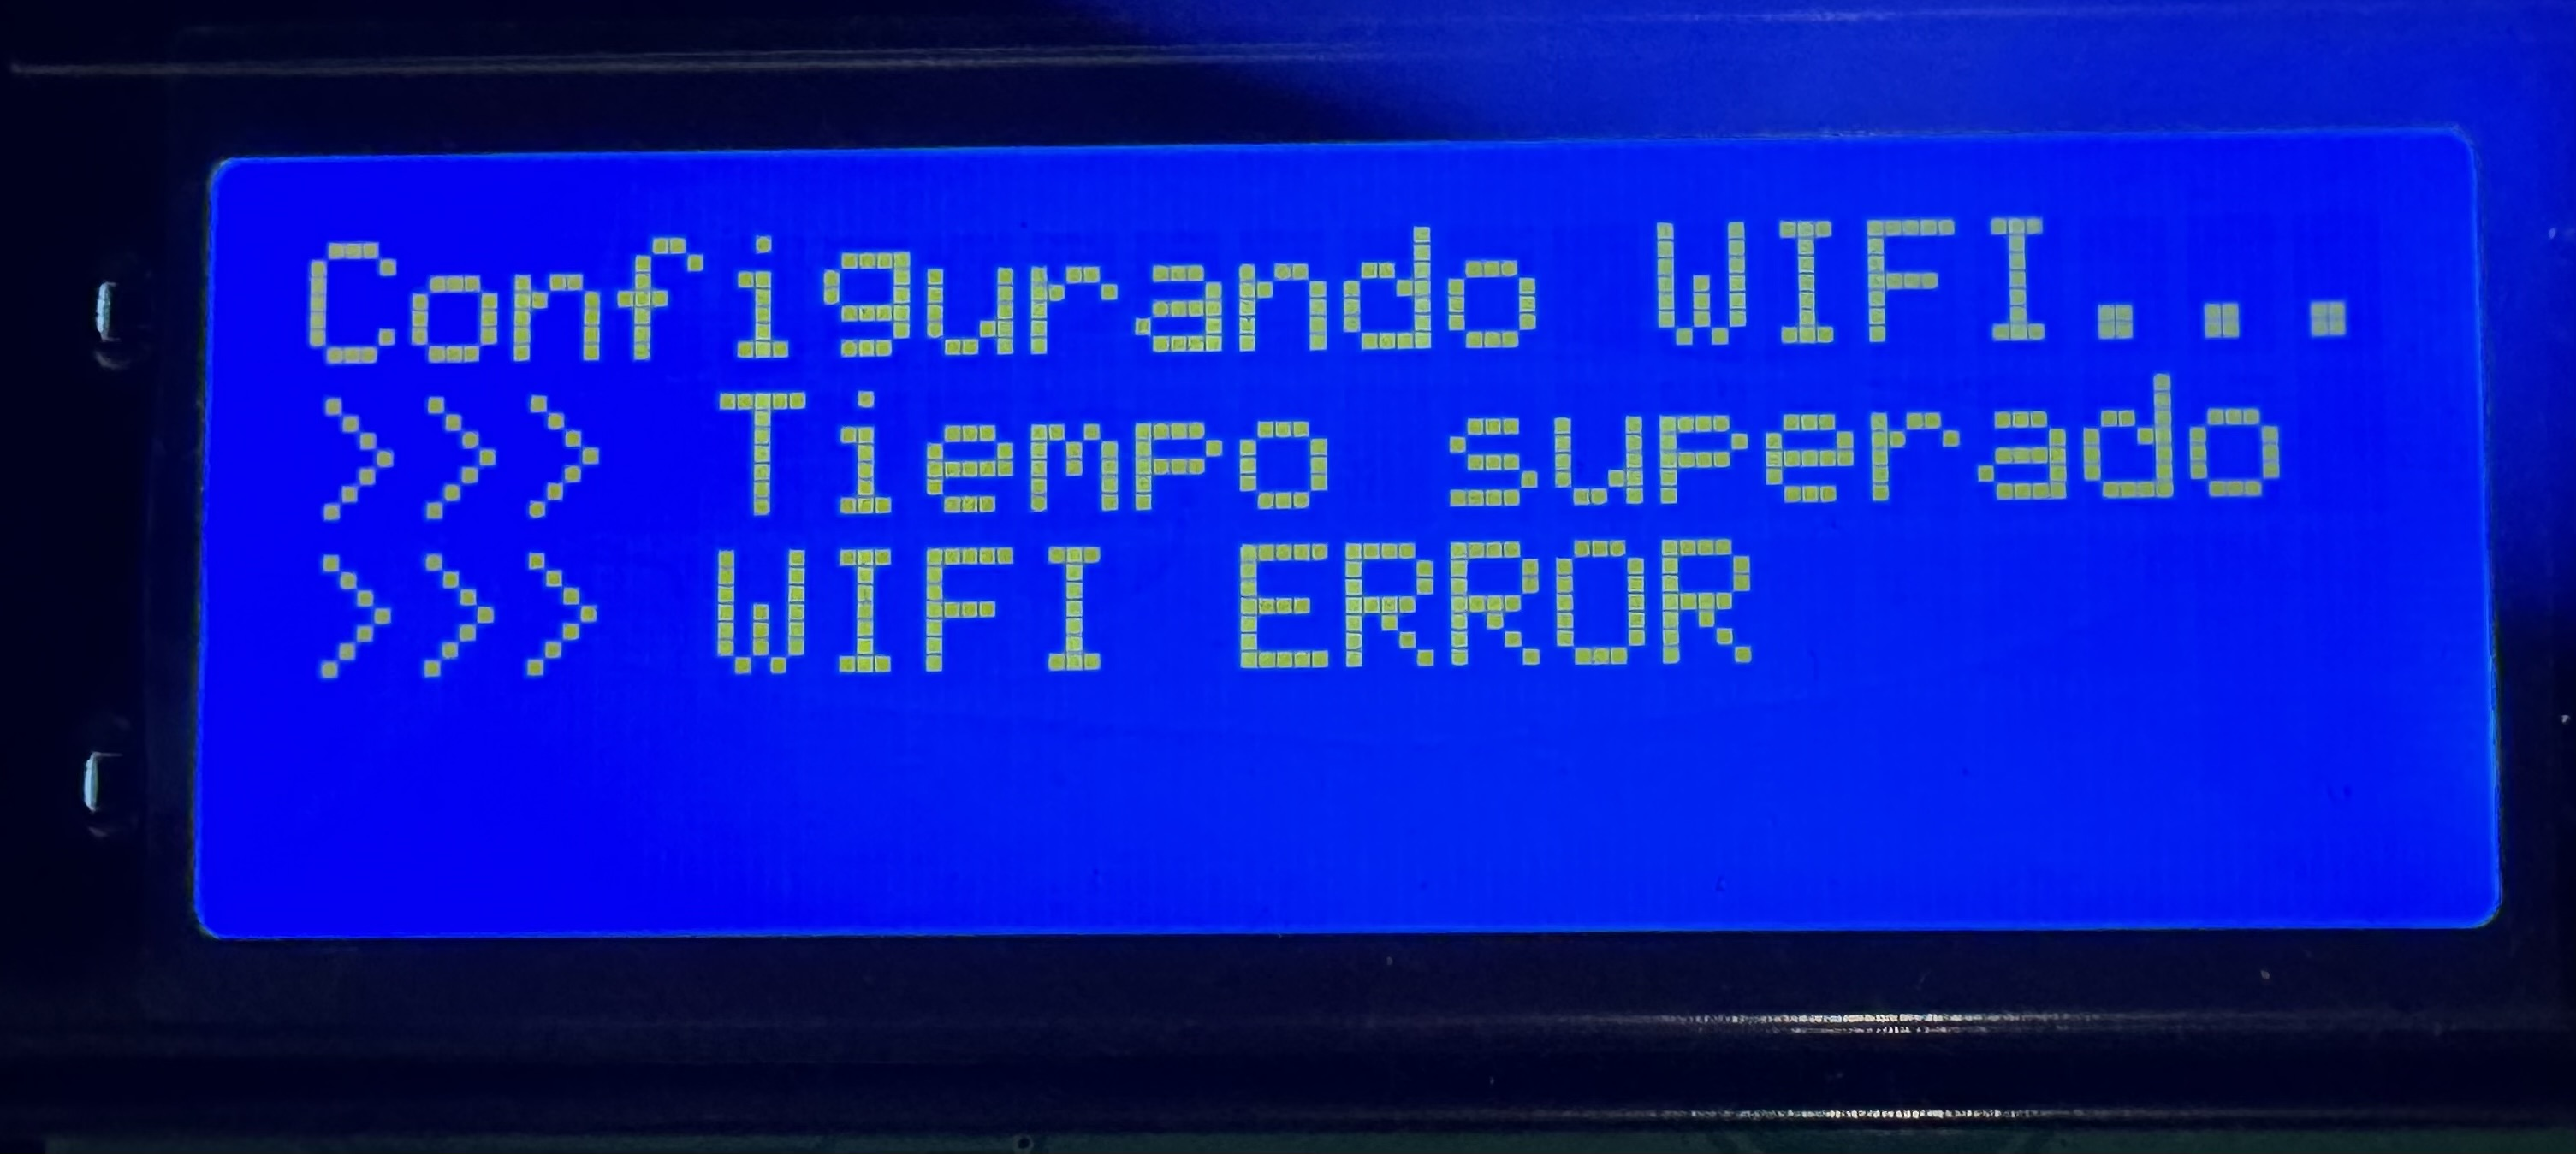
\psfig{file=Figuras/WIFI_ERROR.jpeg,width=8cm,angle=0}} 
\caption{No se ha podido conectar con la red WIFI}\label{patalla:wifiError} 
\end{figure}

Lo volverá a intentar 5 cada vez que quiera mandar un dato.

Si se consigue realizar la conexión con la WIFI aparecerá por pantalla el mensaje (figura \ref{patalla:WifiOk})

\begin{figure}[htbp!] 
\centering{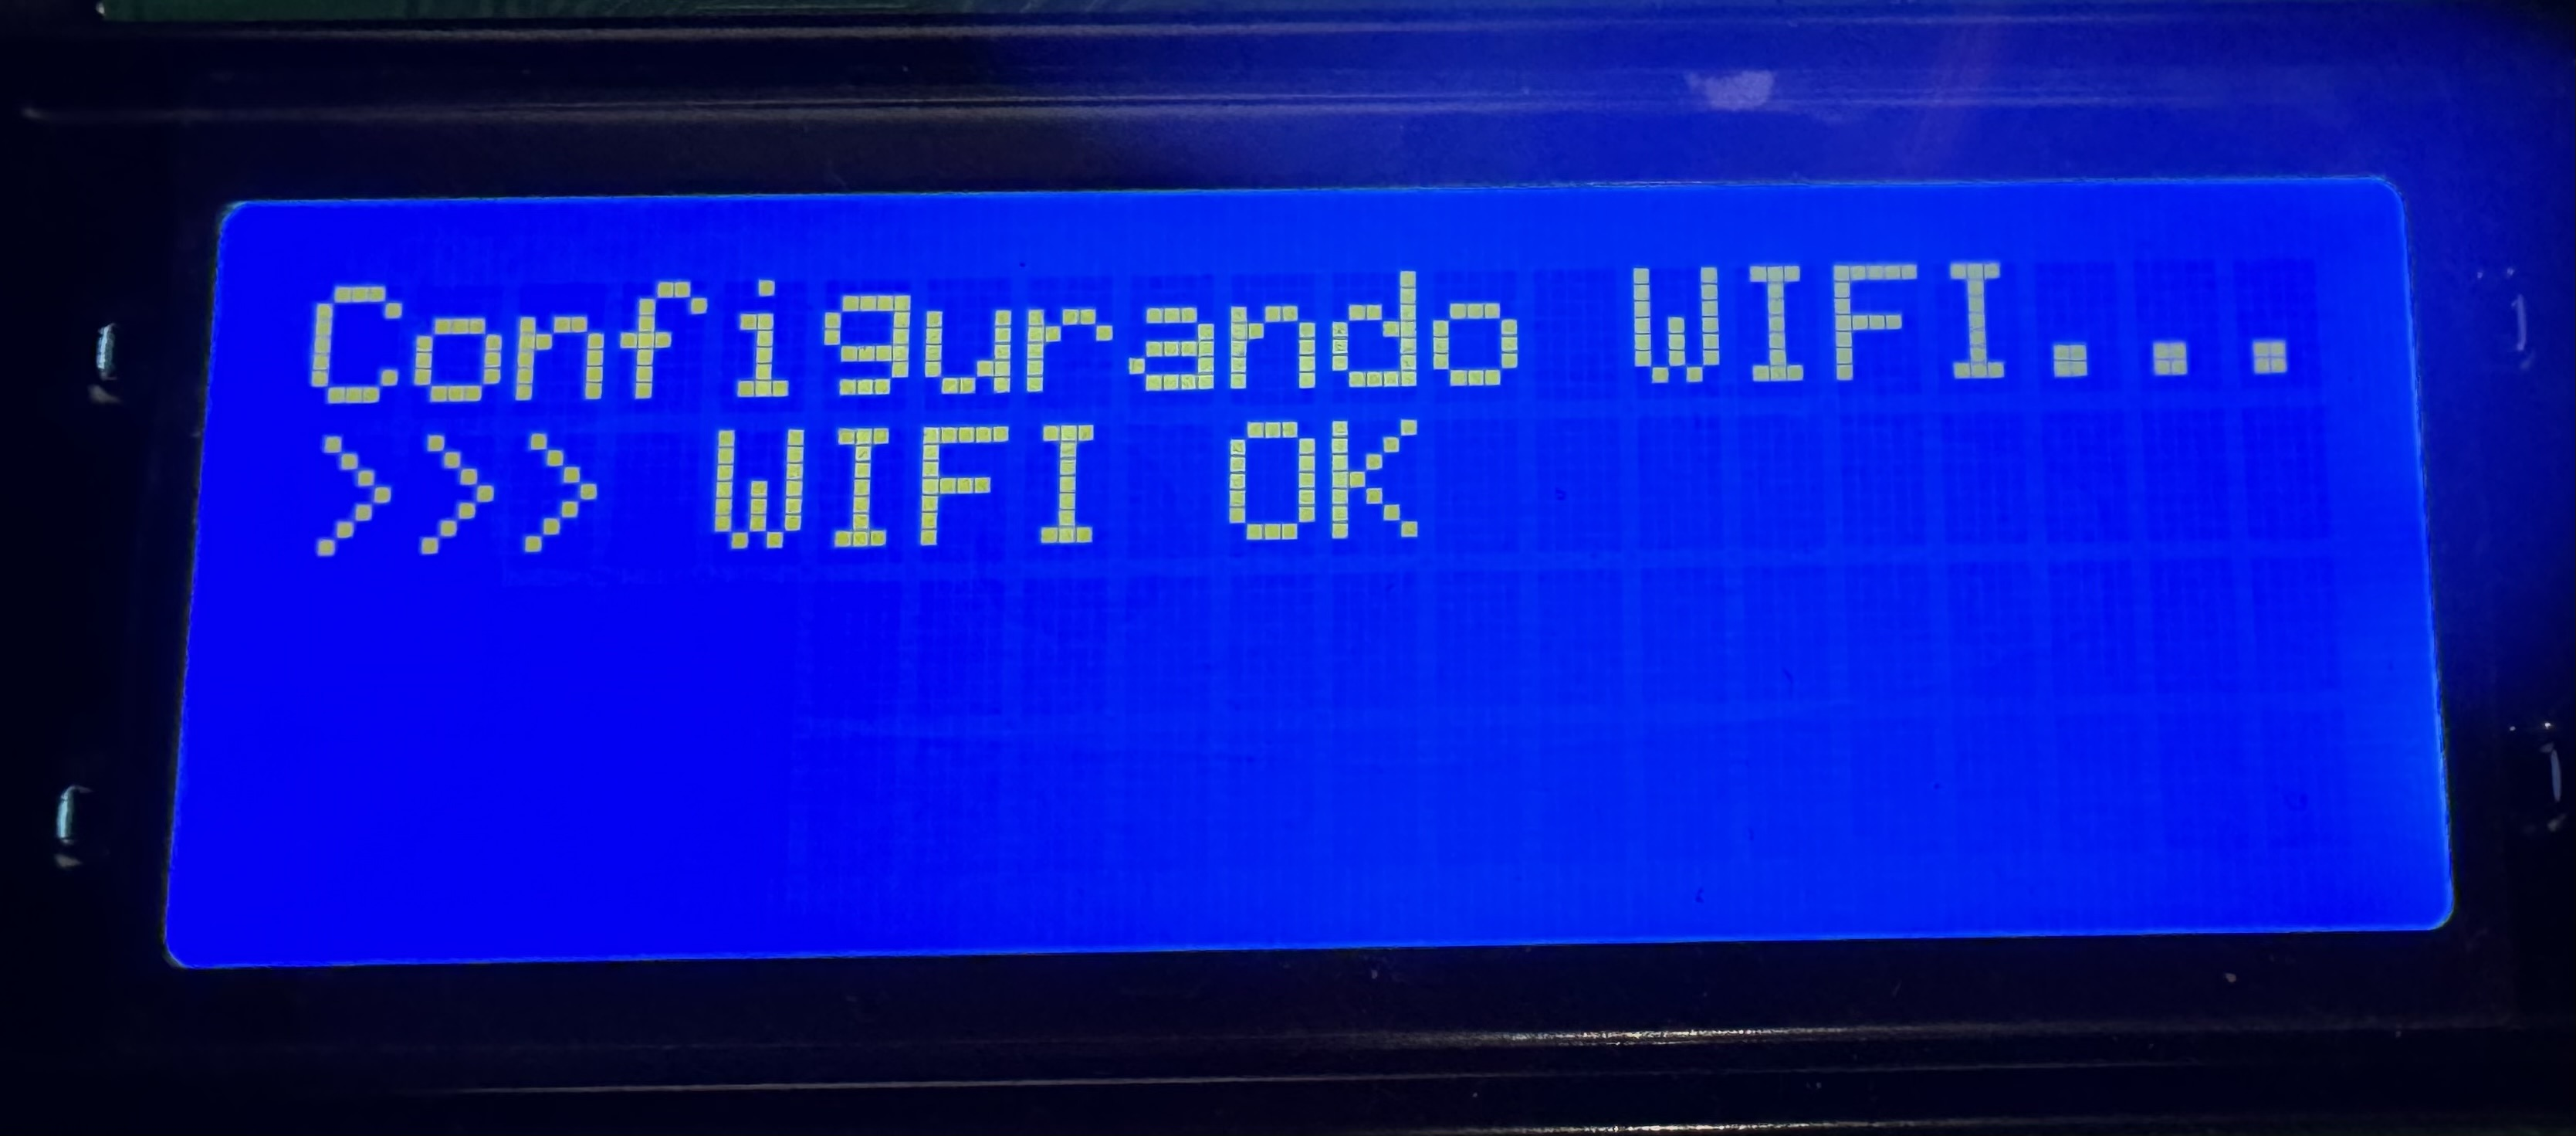
\psfig{file=Figuras/WIFI_OK.jpeg,width=8cm,angle=0}} 
\caption{Cargada la configuración de los sensores}\label{patalla:WifiOk} 
\end{figure}

Se encenderá el led con la etiqueta WIFI de la figura \ref{botones}.

%%%%%%%%%%%%%%%%%%%%%%%%%%%%%%%%%%%%%%%%%%%%%%%%%%%%%%%%%%%%%%%%%%%%%%%%%%%%%%%%%%%%%%%%%%%%%%%%

\item Si se ha podido configurar la WIFI, actualizará la hora interna del módulo de reloj. La actualiza con la hora GMT0 y luego se corregirá en función de donde se encuentre la instalación (figura \ref{patalla:relojOK})

\begin{figure}[htbp!] 
\centering{\psfig{file=Figuras/reloj_OK.jpeg,width=8cm,angle=0}} 
\caption{Módulo de reloj actualizado}\label{patalla:relojOK} 
\end{figure}


%%%%%%%%%%%%%%%%%%%%%%%%%%%%%%%%%%%%%%%%%%%%%%%%%%%%%%%%%%%%%%%%%%%%%%%%%%%%%%%%%%%%%%%%%%%%%%%%

\item A continuación intentará conectarse con el servidor mqtt. Si la WIFI está OK no habrá problemas a no ser que el servidor de Ayesa esté caído. Si no se puede aparecerá la siguiente pantalla (figura \ref{patalla:mqttError})

\begin{figure}[htbp!] 
\centering{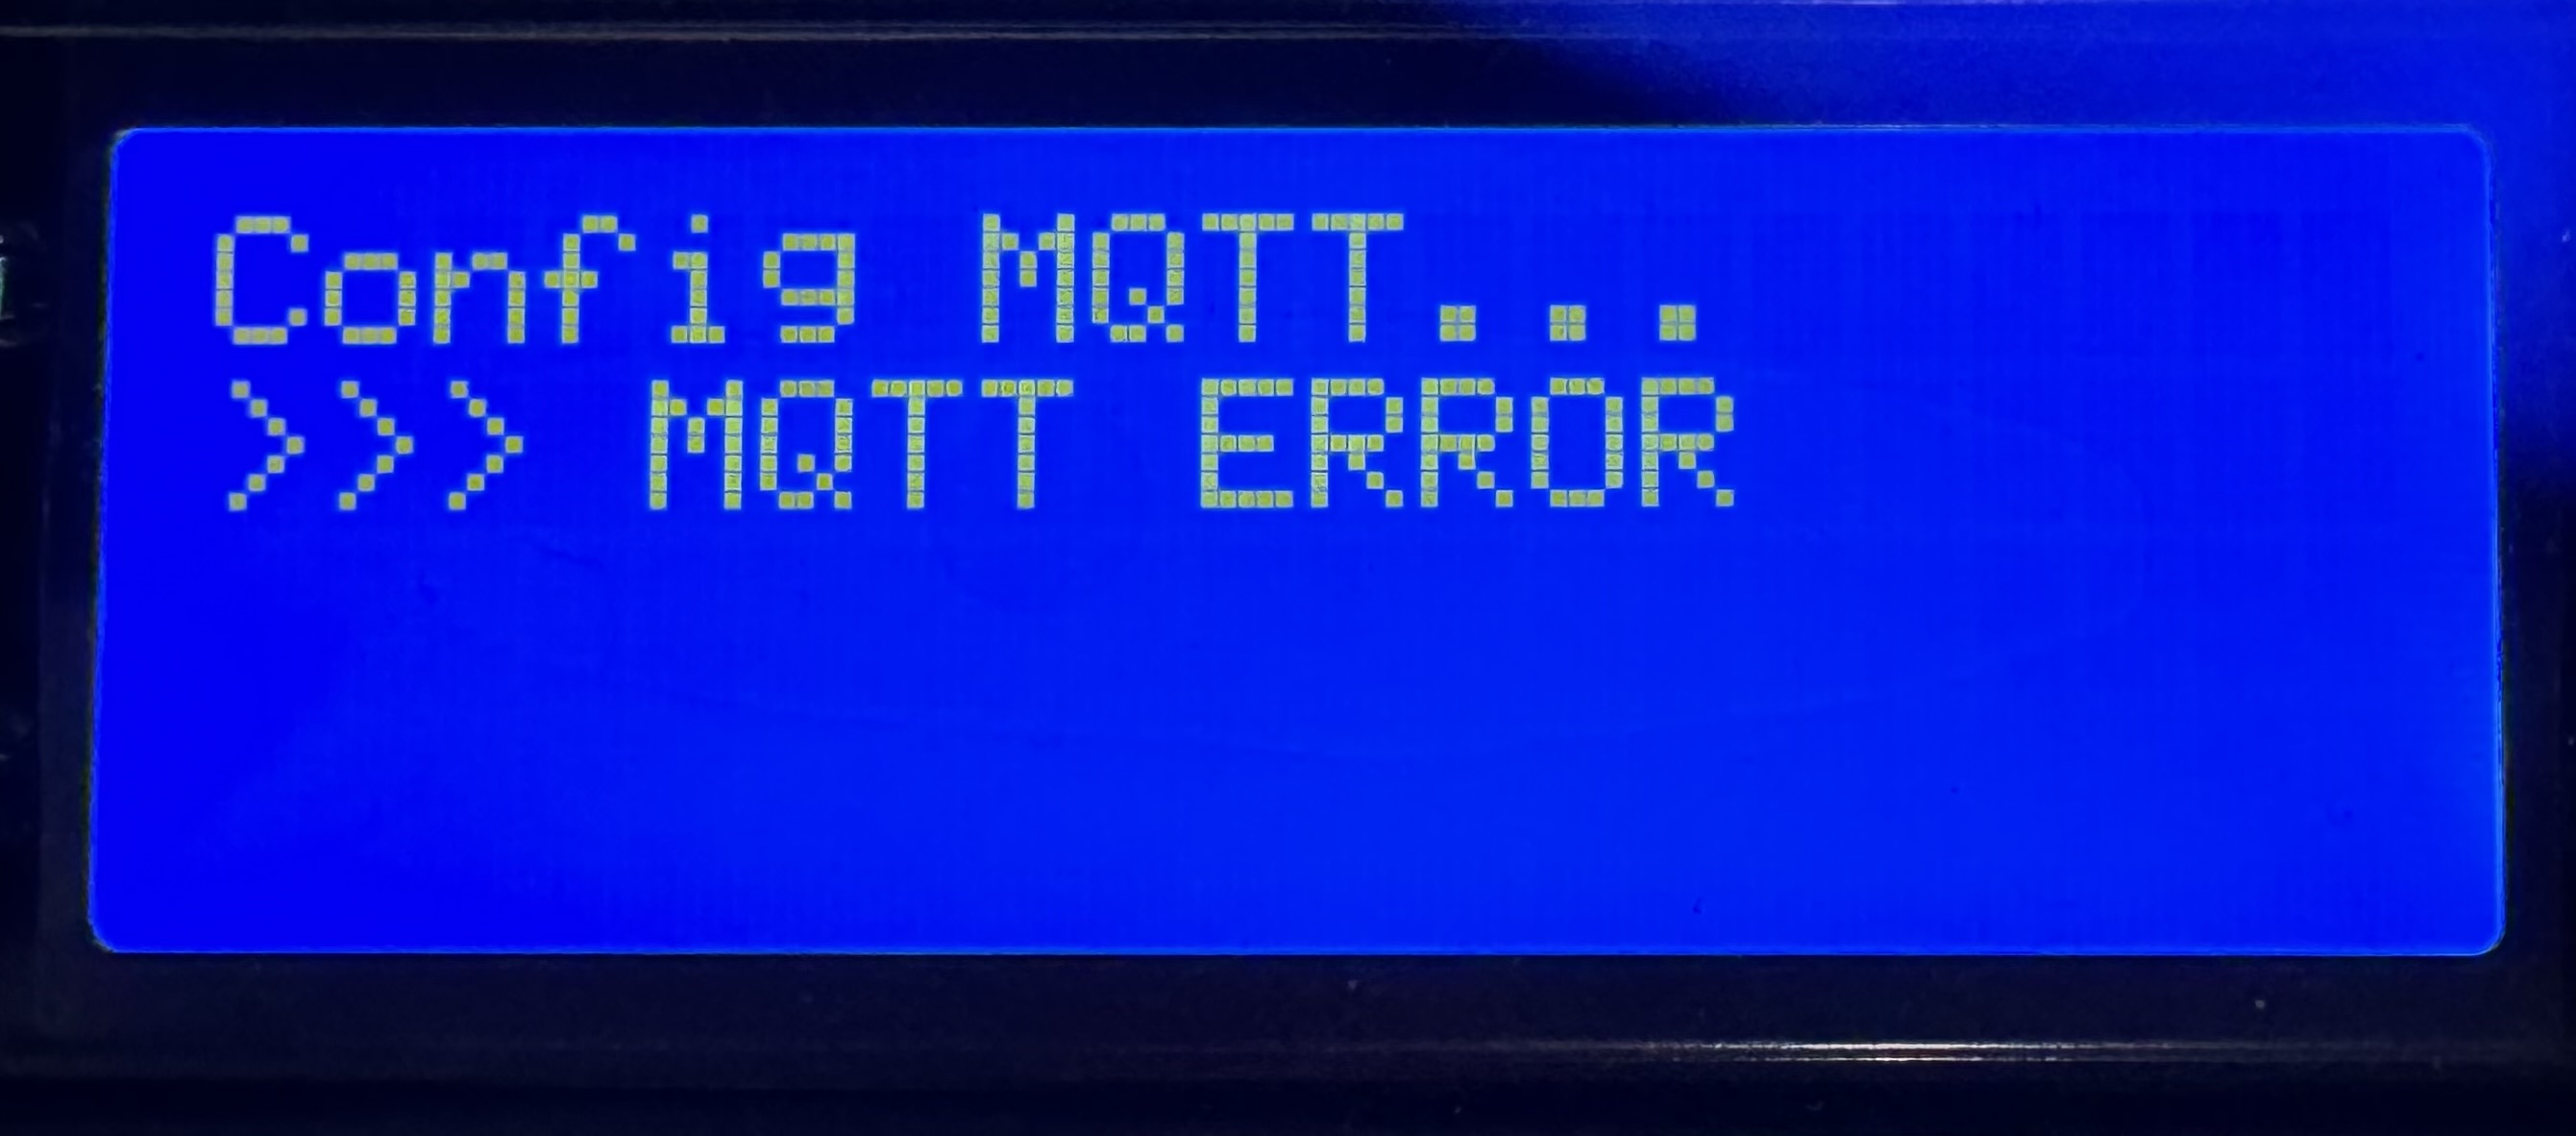
\psfig{file=Figuras/mqtt_ERROR.jpeg,width=8cm,angle=0}} 
\caption{Error al conectarse al sevidor mqtt}\label{patalla:mqttError} 
\end{figure}

Esta tarea requiere cierto tiempo porque lo intentará 5 veces. Durante el funcionamiento normal del dispositivo, cada vez que intente mandar un dato, chequeará el servidor MQTT y si no hay conexión, volverá a intentar conectarse 5 veces.

En caso de que que se conecte, aparecerá pantalla (figura \ref{patalla:mqttOK}). Además se encenderá el led con la etiqueta \emph{MQTT} de la figura \ref{botones}.

\begin{figure}[htbp!] 
\centering{\psfig{file=Figuras/mqtt_OK.jpeg,width=8cm,angle=0}} 
\caption{Éxito al conectarse al sevidor mqtt}\label{patalla:mqttOK} 
\end{figure}

%%%%%%%%%%%%%%%%%%%%%%%%%%%%%%%%%%%%%%%%%%%%%%%%%%%%%%%%%%%%%%%%%%%%%%%%%%%%%%%%%%%%%%%%%%%%%%%%

\item A continuación entra en el modo de funcionamiento normal, donde aparecerán dos pantallas que alternan cada 5 segundos. La primera muestra las variables relacionadas con el agua y la segunda con el aire.

En la pantalla\footnote{Los valores que aparecen en la pantalla no son reales pues cuando se hizo esta guía el dispositivo no tenía sensores conectados} relacionada con el agua puede verse (figura \ref{patalla:1}):
\begin{itemize}
\item Línea 1: hora y fecha
\item Línea 2: temperatura TW1 que es la temperatura de la sonda de conductividad. Y la temperatura TW2 es la temperatura proporcionada por el sensor DS18B20.
\item Línea 3: Valor de la conductividad
\item Línea 4: valor del PH y de la concentración de $O_2$
\end{itemize}

\begin{figure}[htbp!] 
\centering{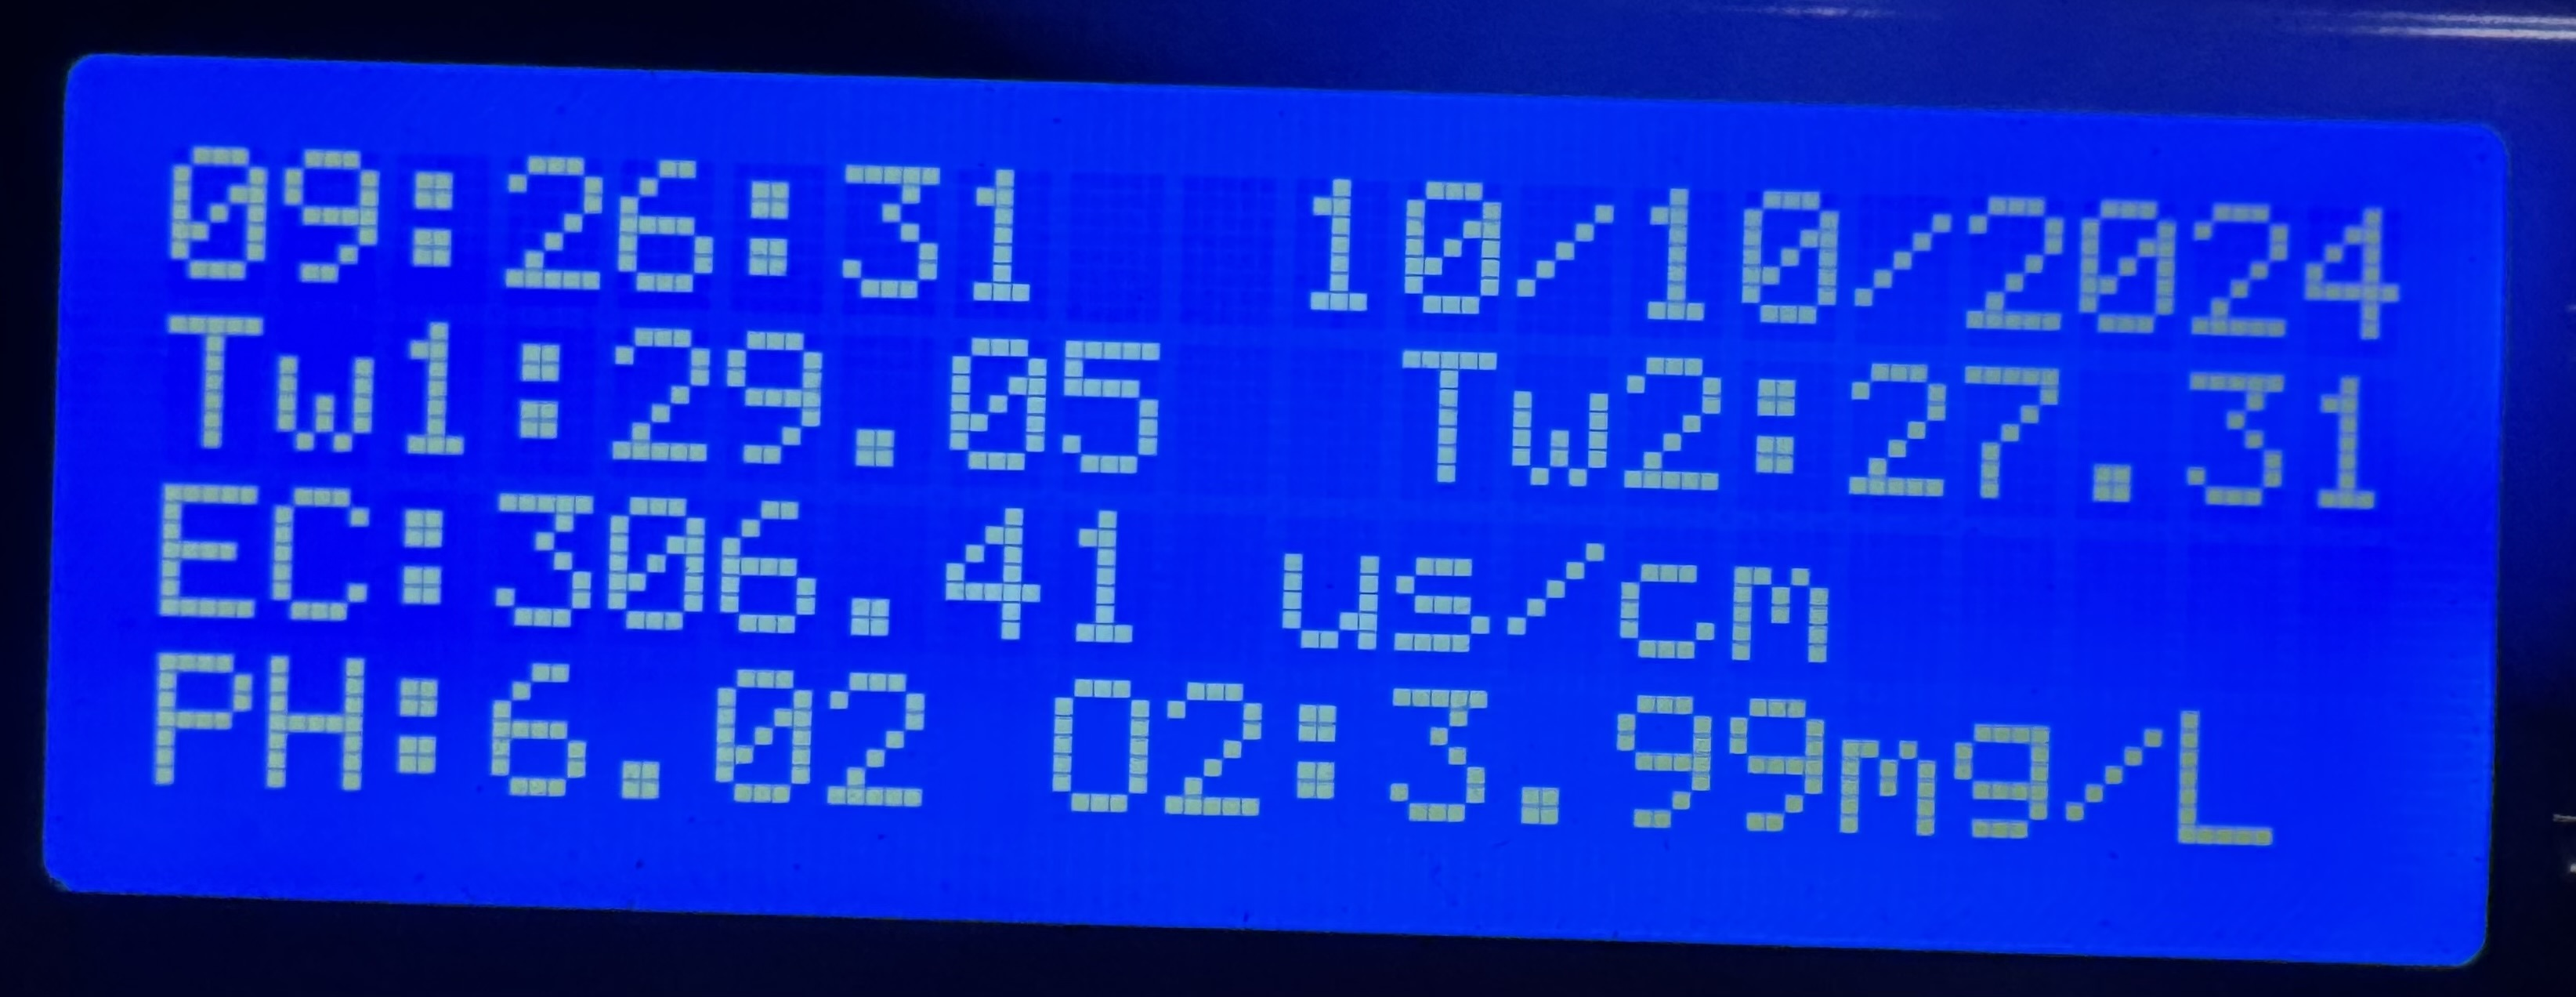
\psfig{file=Figuras/pantalla1.jpeg,width=8cm,angle=0}} 
\caption{Pantalla que muestra las variables relacionadas con el agua}\label{patalla:1} 
\end{figure}

En la pantalla relacionada con el agua puede verse (figura \ref{patalla:2}):
\begin{itemize}
\item Línea 1: hora y fecha
\item Línea 2: VAR AMB, para recordar que son variables ambientales.
\item Línea 3: Valores de temperatura y humedad del aire del sensor DTH22 conectado en el puerto de la placa DTH22A.
\item Línea 4: Valores de temperatura y humedad del aire del sensor DTH22 conectado en el puerto de la placa DTH22B.
\end{itemize}

\begin{figure}[htbp!] 
\centering{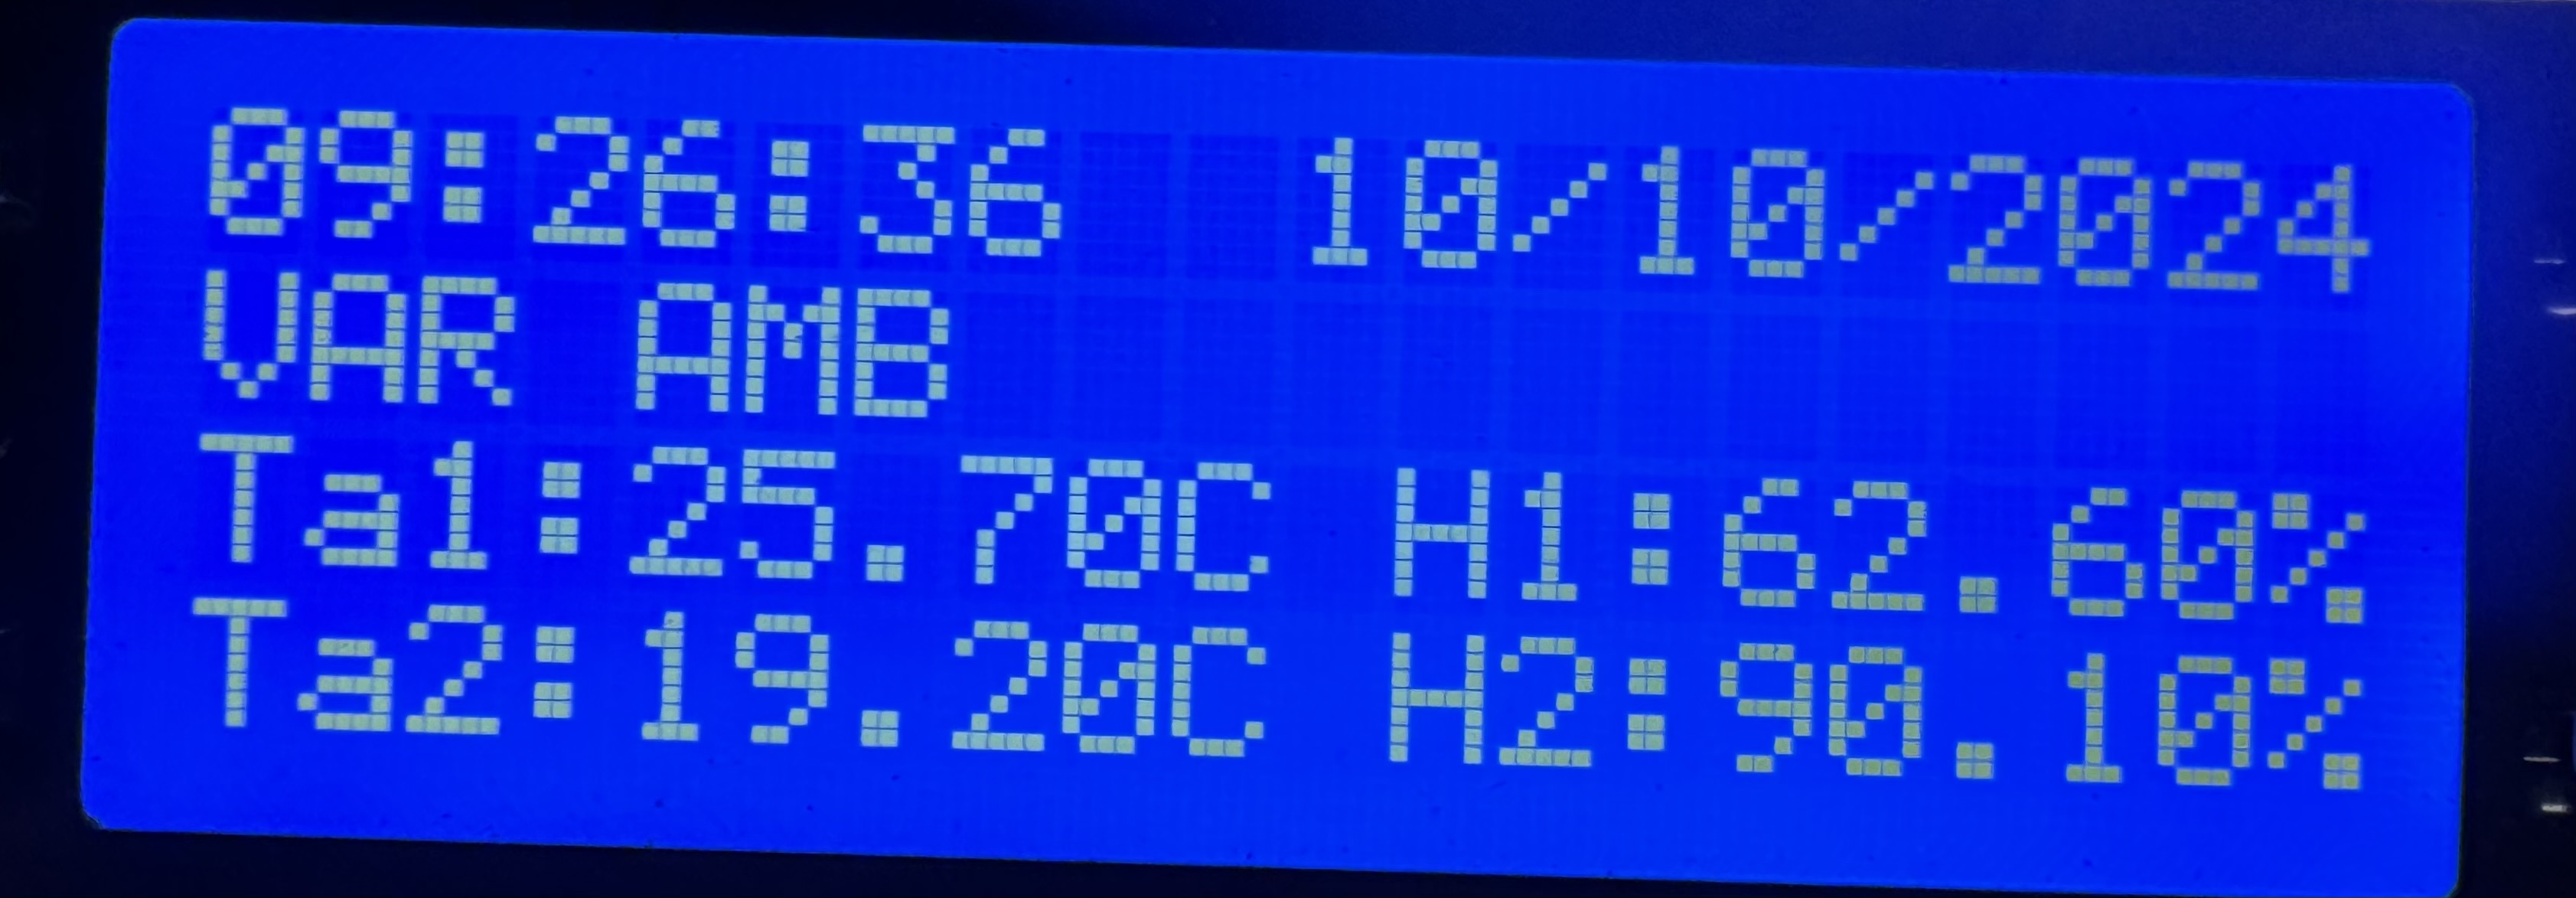
\psfig{file=Figuras/pantalla2.jpeg,width=8cm,angle=0}} 
\caption{Pantalla que muestra las variables relacionadas con el aire}\label{patalla:2} 
\end{figure}

\end{enumerate}

%%%%%%%%%%%%%%%%%%%%%%%%%%%%%%%%%%%%%%%%%%%%%%%%%%%%%%%%%%%%%%%%%%%%%%%%%%%%%%%%%%%%%%%%%%%%%%%%
\newpage
\section{Sensor de PH y calibración}

El sensor que se usa en este proyecto es un DFRobot SEN0169-V2 en su versión con probeta industrial:
\begin{verbatim}
https://www.dfrobot.com/product-2069.html
https://wiki.dfrobot.com/Gravity__Analog_pH_Sensor_Meter_Kit_V2_SKU_SEN0161-V2
\end{verbatim}
El medidor de pH analógico por gravedad V2 de DFRobot está diseñado específicamente para medir el pH de una solución y reflejar su acidez o alcalinidad. La señal de salida se filtra por hardware y tiene una fluctuación general baja.

El sensor de PH nos dará una tensión que va de 0V a 3V. El fabricante dice que el PH y la tensión tiene una relación lineal por lo que con tener dos punto de esa recta sería suficiente para poder calibrar dicho sensor. 
\subsection{Primer punto de la recta de PH}

Una vez estamos en la pantalla principal pulsamos el botón MODE una única vez\footnote{Si se pasa la pantalla, siga pulsando hasta que vuelva la pantalla principal} hasta que sale la pantalla (figura \ref{patalla:PH1}). Fíjese que es la parte superior aparece la frase: \textbf{CAL PH1}.

\begin{figure}[htbp!] 
\centering{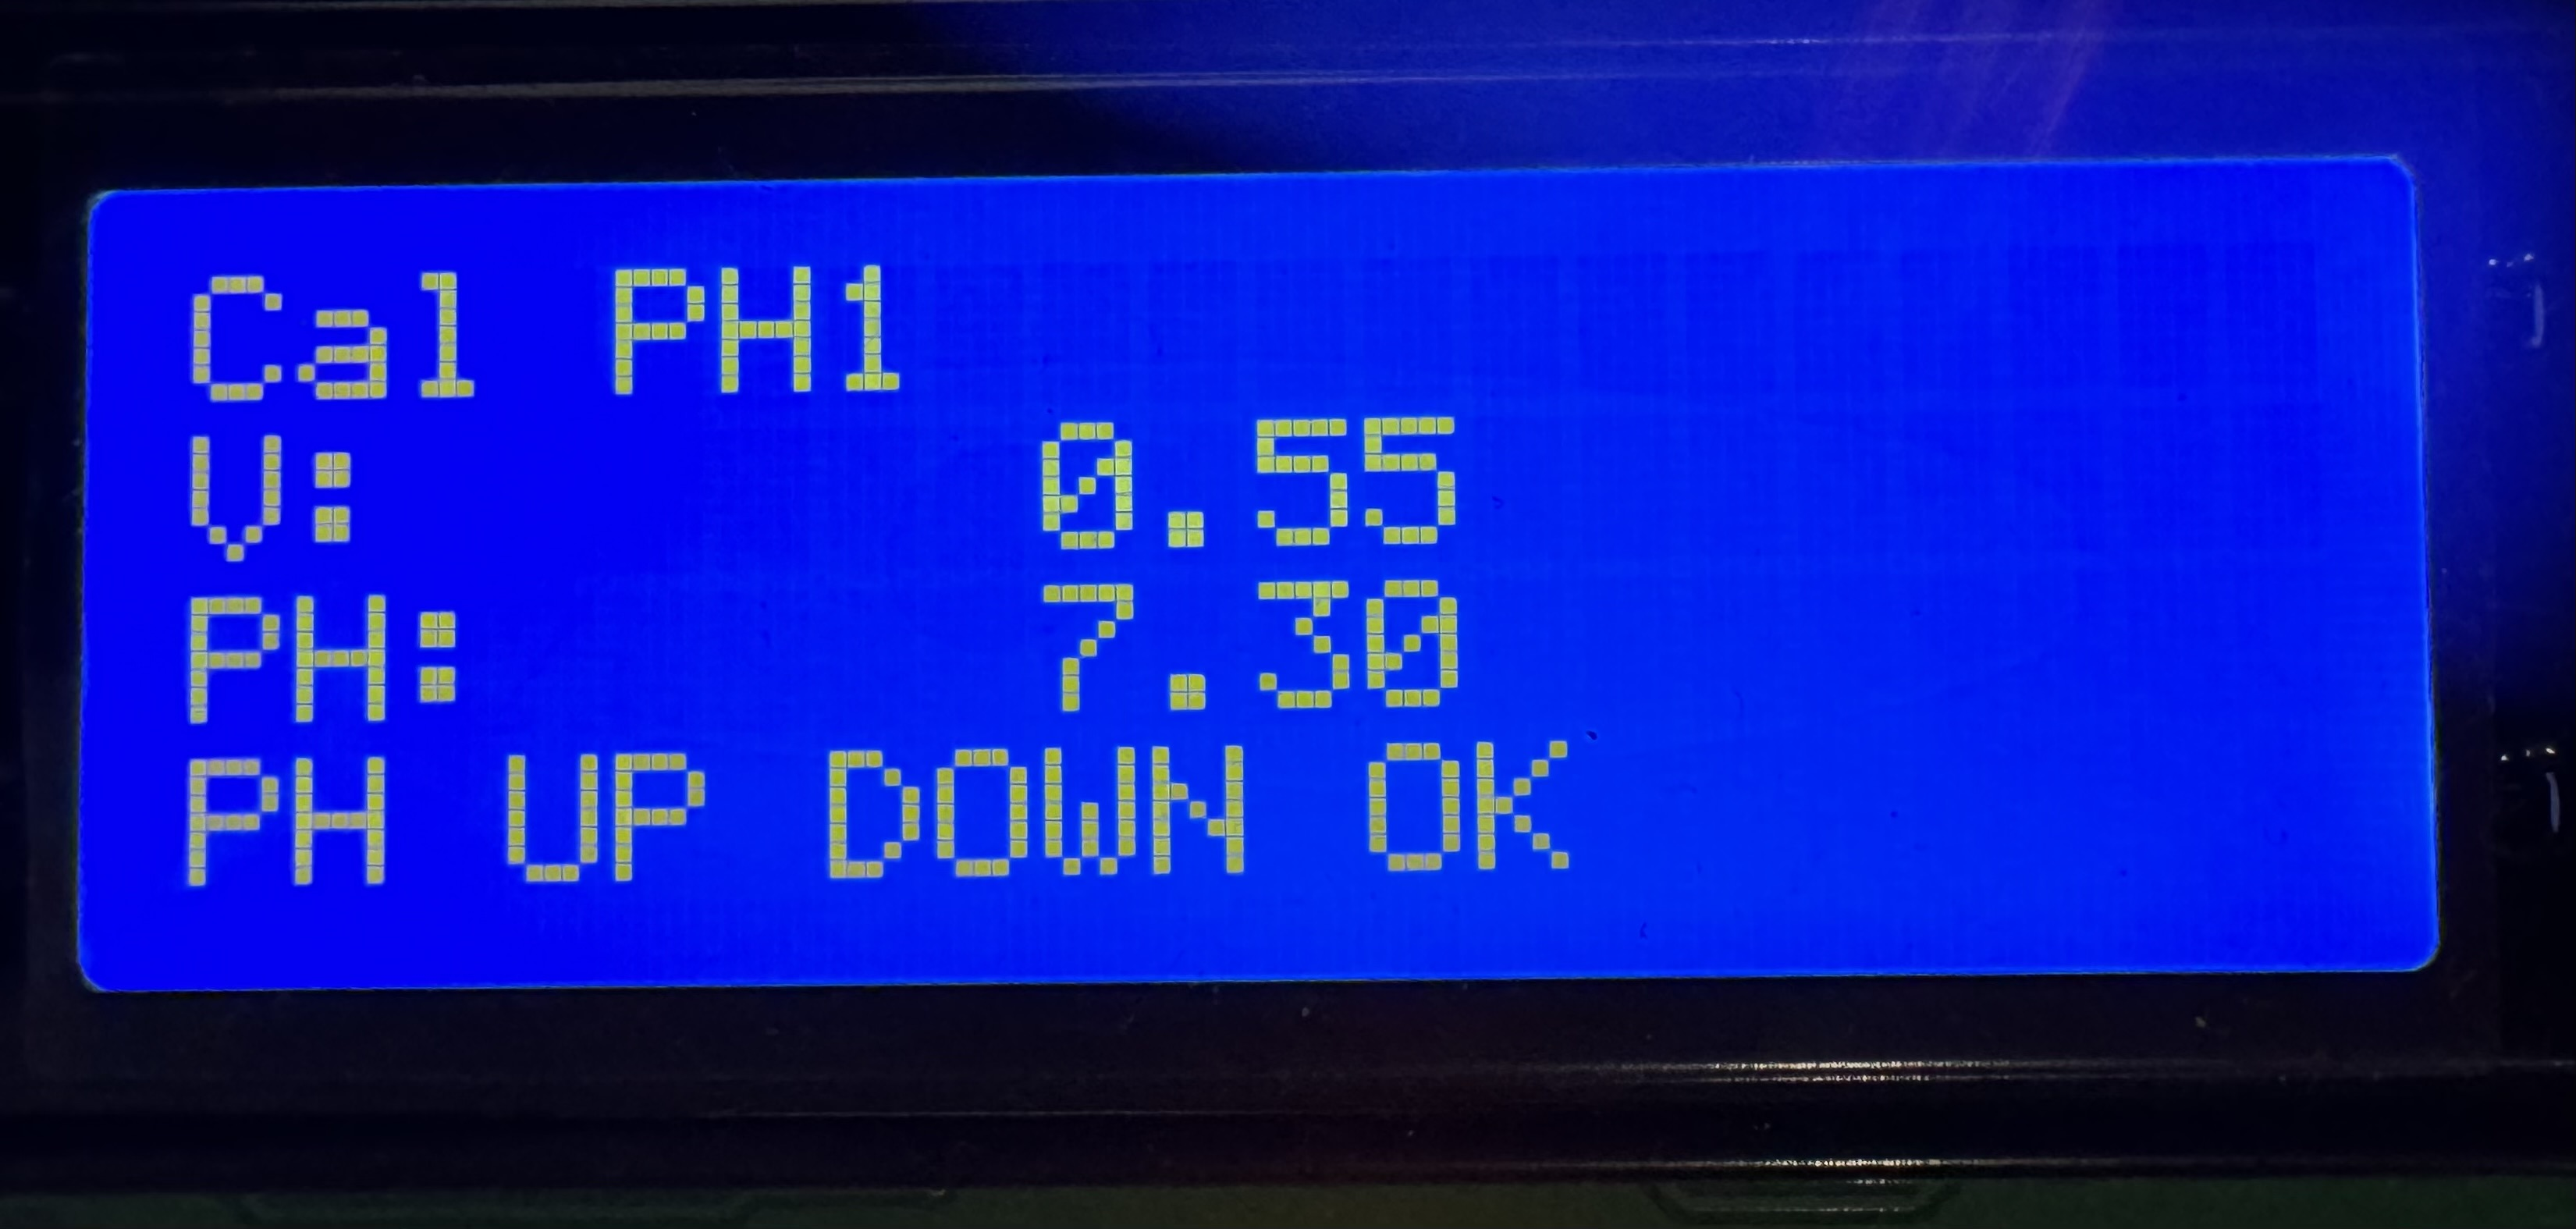
\psfig{file=Figuras/PH1.jpeg,width=8cm,angle=0}} 
\caption{Primer punto de calibración del sensor de PH}\label{patalla:PH1} 
\end{figure}

\begin{itemize}
\item Línea 1: \textbf{CAL PH1}.
\item Línea 2: \textbf{V:} es la tensión que está leyendo el sensor.
\item Línea 3: \textbf{PH:}Valor de PH de ese punto (lo establecemos pulsando UP o DOWN para incrementar o decrementar dicho valor 0.1. 
\item Línea 4: \textbf{PH UP DOWN OK}. Podemos variar el PH con UP o DOWN y una vez que este todo pulsamos OK para acabar.
\end{itemize}

El procedimiento es el siguiente: Metemos la probeta del PH previa limpieza en un líquido de PH conocido y \underline{esperamos un minuto} a que se estabilice la tensión. Ajustamos el campo PH con UP y DOWN y pulsamos OK. En ese momento se ajusta el primer punto de la recta característica del sensor de PH. 

En el archivo \emph{config.txt} se actualizaran los valores \emph{PH1} y \emph{mV1}.

\subsection{Segundo punto de la recta de PH}

Una vez estamos en la pantalla principal pulsamos el botón MODE dos veces\footnote{Si se pasa la pantalla, siga pulsando hasta que vuelva la pantalla principal} hasta que sale la pantalla (figura \ref{patalla:PH2}). Fíjese que es la parte superior aparece la frase: \textbf{CAL PH2}.

\begin{figure}[htbp!] 
\centering{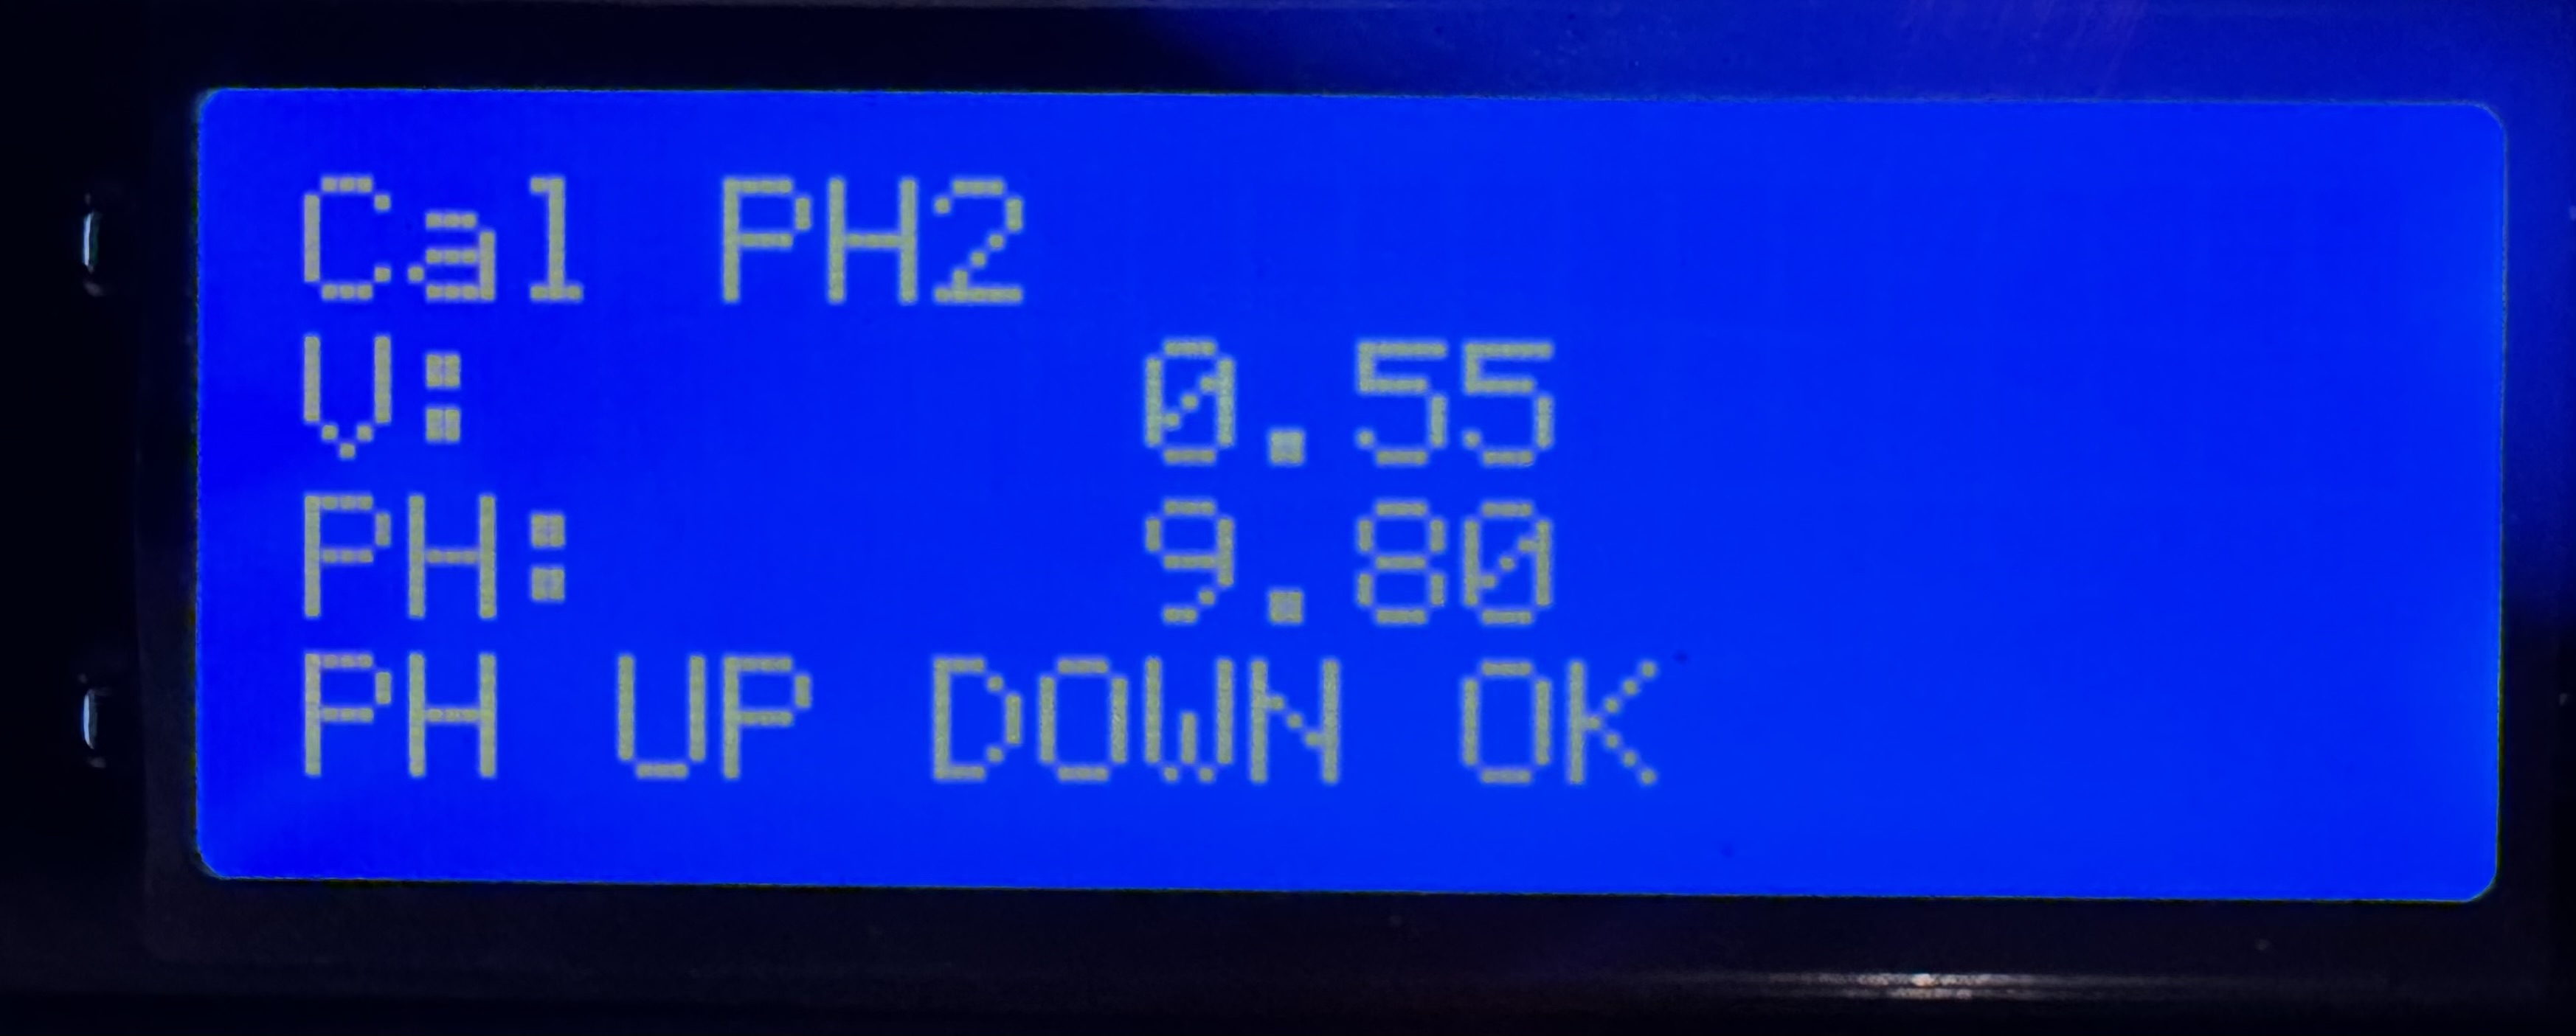
\psfig{file=Figuras/PH2.jpeg,width=8cm,angle=0}} 
\caption{Segundo punto de calibración del sensor de PH}\label{patalla:PH2} 
\end{figure}

\begin{itemize}
\item Línea 1: \textbf{CAL PH2}.
\item Línea 2: \textbf{V:} es la tensión que está leyendo el sensor.
\item Línea 3: \textbf{PH:}Valor de PH de ese punto (lo establecemos pulsando UP o DOWN para incrementar o decrementar dicho valor 0.1. 
\item Línea 4: \textbf{PH UP DOWN OK}. Podemos variar el PH con UP o DOWN y una vez que este todo pulsamos OK para acabar.
\end{itemize}

El procedimiento es el siguiente: Metemos la probeta del PH, previa limpieza, en el segundo líquido de PH conocido (con un  PH distinto del primero) y \underline{esperamos un minuto} a que se estabilice la tensión. Ajustamos el campo PH con UP y DOWN y pulsamos OK. En ese momento se ajusta el segundo punto de la recta característica del sensor de PH. 

En el archivo \emph{config.txt} se actualizaran los valores \emph{PH2} y \emph{mV2}.

\begin{tcolorbox}
[colback=red!5!white,colframe=red!75!black,fonttitle=\bfseries,title=CALIBRACIÓN SENSOR PH]
Este sensor se ha estado usando durante más de un año y como mejores resultados ha dado es:
\begin{enumerate}
\item Escogemos el primer punto de calibración un punto del PH típico, usando el propio baño de los peces como líquido de calibración. Medimos el PH con un sensor portátil y ajustamos el primer punto con dicho valor. Se chequea el valor del PH una vez al día y si hay desviación se corrige el punto 1 del sensor sobre la marcha.
\item El segundo punto hay que hacerlo con un PH ácido con una solución de PH conocido. la misma que se utiliza para calibrar el sensor de PH portátil. Este punto se recalibra una vez al mes como dice el fabricante.
\end{enumerate}
Según el fabricante la vida de la probeta es de 1 año. Mi experiencia es que haciendo frecuentes recalibraciones, la recta característica se va adaptando al deterioro de la sonda. Y dado que el PH no varía mucho se puede aguantar más tiempo.

\end{tcolorbox}




%%%%%%%%%%%%%%%%%%%%%%%%%%%%%%%%%%%%%%%%%%%%%%%%%%%%%%%%%%%%%%%%%%%%%%%%%%%%%%%%%%%%%%%%%%%%%%%%%%%%%%

\newpage
\section{Sensor de concentración de O2 y calibración}

El sensor que se usa en este proyecto es un DFRobot Sensor de oxigeno disuelto SEN0237-A. El sensor de oxígeno disuelto SEN0237-A es compatible con tarjetas Arduino. Se utiliza para medir la concentración de oxígeno en el agua. Este parámetro permite identificar la calidad del agua. Una baja concentración de oxígeno en el agua producirá una dificultad de respirar en organismos acuáticos. 
\begin{verbatim}
https://www.dfrobot.com/product-1628.html
https://wiki.dfrobot.com/Gravity__Analog_Dissolved_Oxygen_Sensor_SKU_SEN0237
\end{verbatim}

Hay tres procedimientos de calibración, pero para este proyecto solo se han programado dos de ellos:

\subsection{Procedimiento 1. Usando temperatura del aire}
Este es el procedimiento más sencillo y el que mejores resultados nos ha dado.
\begin{enumerate}
\item Una vez estamos en la pantalla principal pulsamos el botón MODE tres veces\footnote{Si se pasa la pantalla, siga pulsando hasta que vuelva la pantalla principal} hasta que sale la pantalla (figura \ref{patalla:O2aire}). Fíjese que es la parte superior aparece la frase: \textbf{Cal 02 T aire}.

\begin{figure}[htbp!] 
\centering{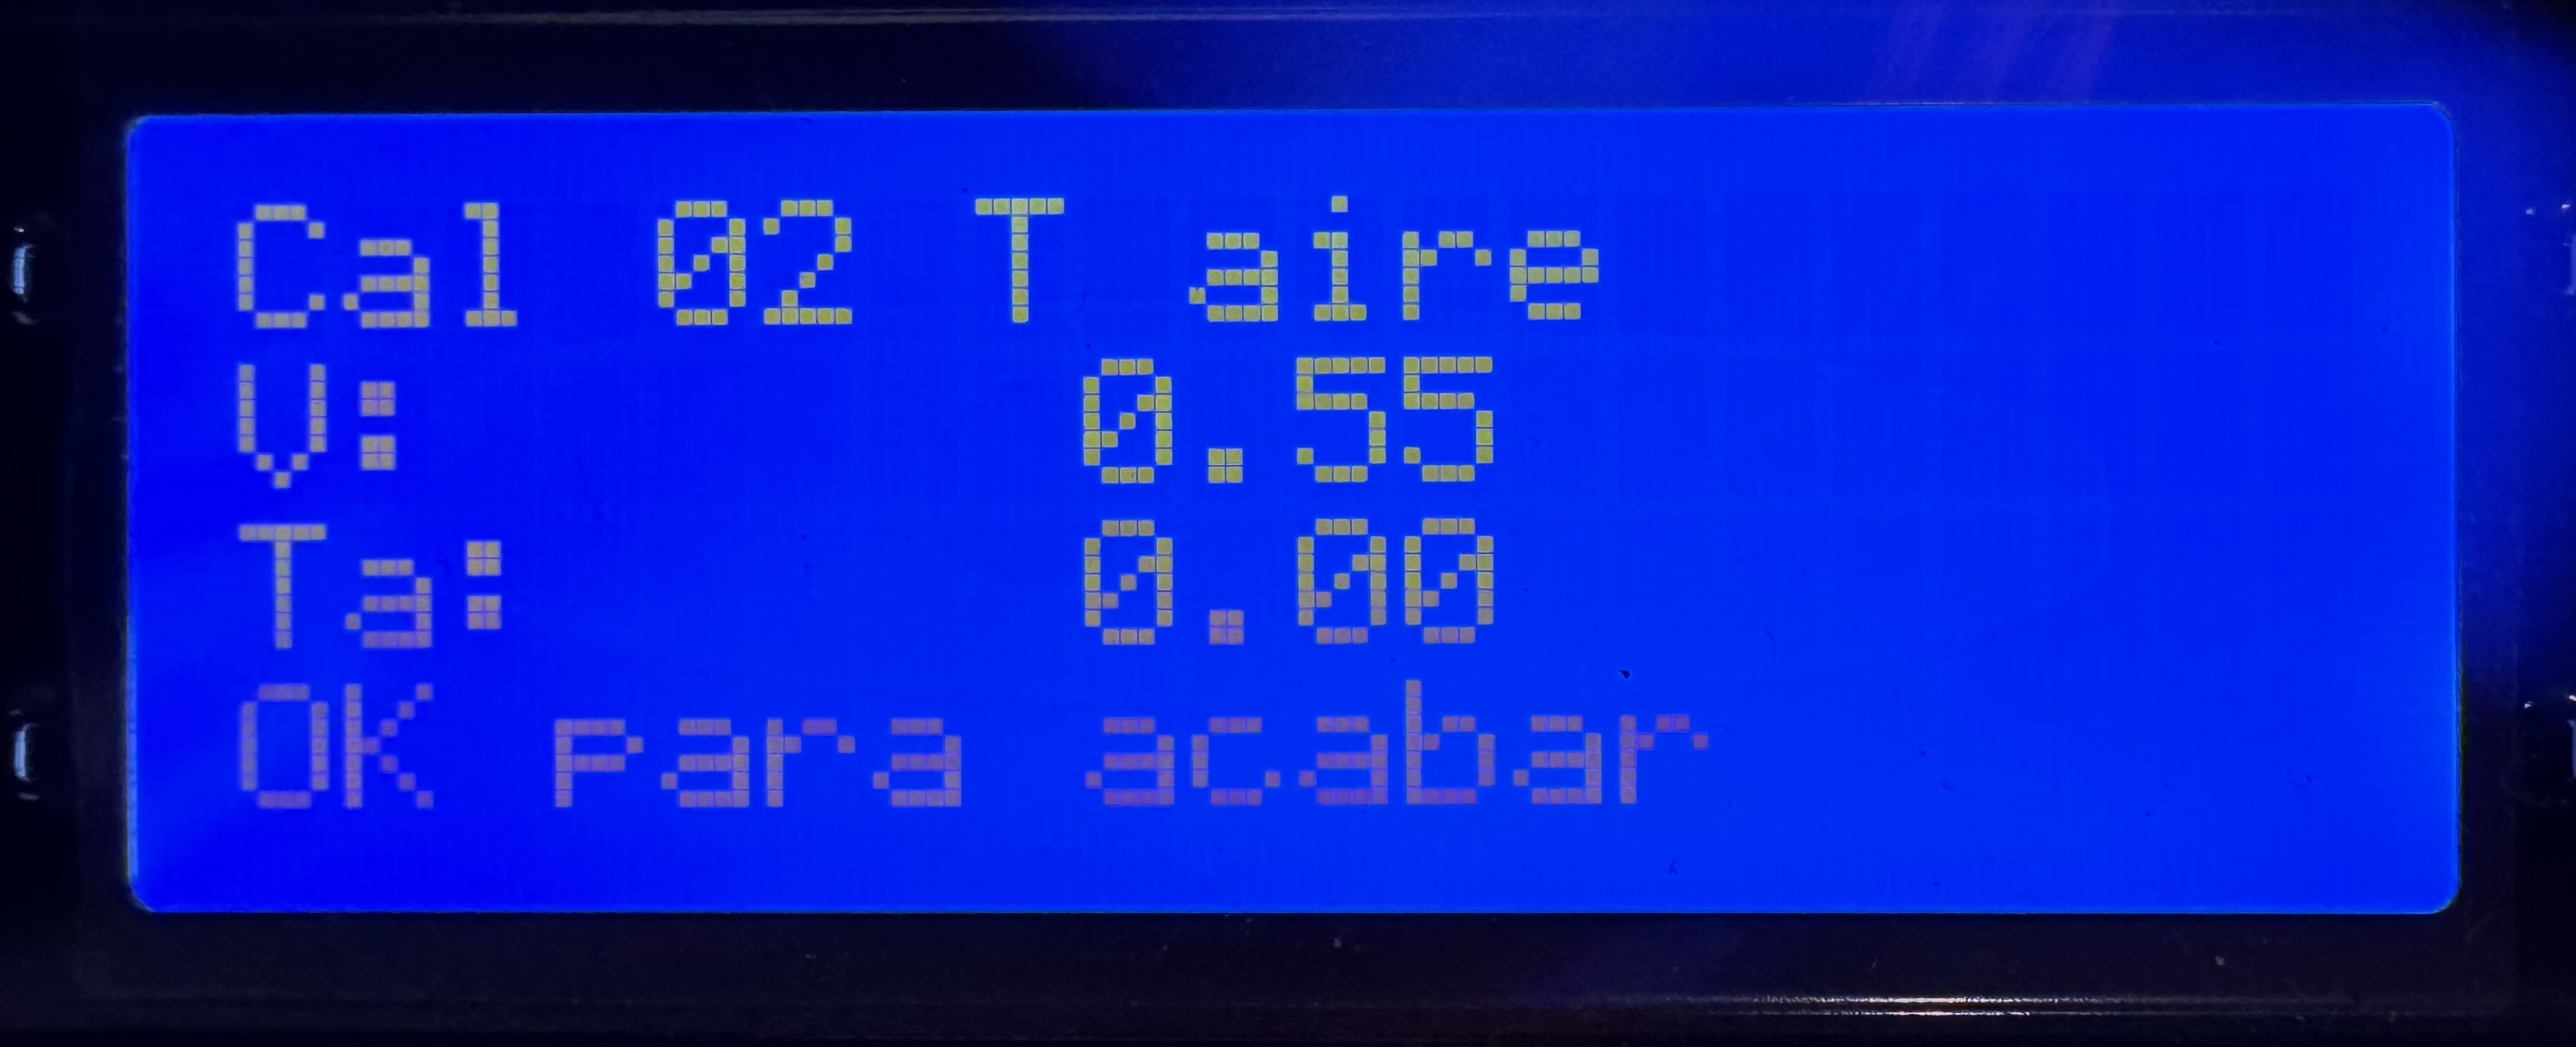
\psfig{file=Figuras/O2aire.jpeg,width=8cm,angle=0}} 
\caption{$1^{er}$ procedimiento para la calibración del sensor de concentración de $O_2$}\label{patalla:O2aire} 
\end{figure}

\begin{itemize}
\item Línea 1: \textbf{Cal 02 T aire}.
\item Línea 2: \textbf{V:} es la tensión que está leyendo el sensor.
\item Línea 3: \textbf{Ta:} El valor de la temperatura del aire proporcionado por el sensor DTH22 conectado el puerto DTH22A. 
\item Línea 4: \textbf{OK para acabar}. Una vez que este todo pulsamos OK para acabar.
\end{itemize}

\item Moja la probeta en agua pura y agítala para que elimine el exceso de agua. Expón la probeta al aire y mantenla en una suave corriente de aire durante un minuto, no uses un ventilador. Cuando el voltaje sea estable pulsa OK. Este procedimiento busca el punto de saturación de oxigeno del agua a una determinada temperatura.

En el archivo \emph{config.txt} se actualizaran los valores \emph{CAL1\_V} y \emph{CAL1\_T}\footnote{Verá que en \emph{config.txt} existen también \emph{CAL2\_V} y \emph{CAL2\_T} para ver al influencia de la temperatura. Pero para ello habría que tener aire a dos temperaturas distintas o agua saturada de O2 a dos temperaturas distintas. Este es el tercer procedimiento que se abandonó por la complejidad del mismo.}.
\end{enumerate}

\subsection{Procedimiento 2. Usando temperatura del agua}
Este es el procedimiento más complicado y el que peores resultados nos ha dado.
\begin{enumerate}
\item Una vez estamos en la pantalla principal pulsamos el botón MODE 4 veces\footnote{Si se pasa la pantalla, siga pulsando hasta que vuelva la pantalla principal} hasta que sale la pantalla (figura \ref{patalla:O2agua}). Fíjese que es la parte superior aparece la frase: \textbf{Cal 02 T agua}.

\begin{figure}[htbp!] 
\centering{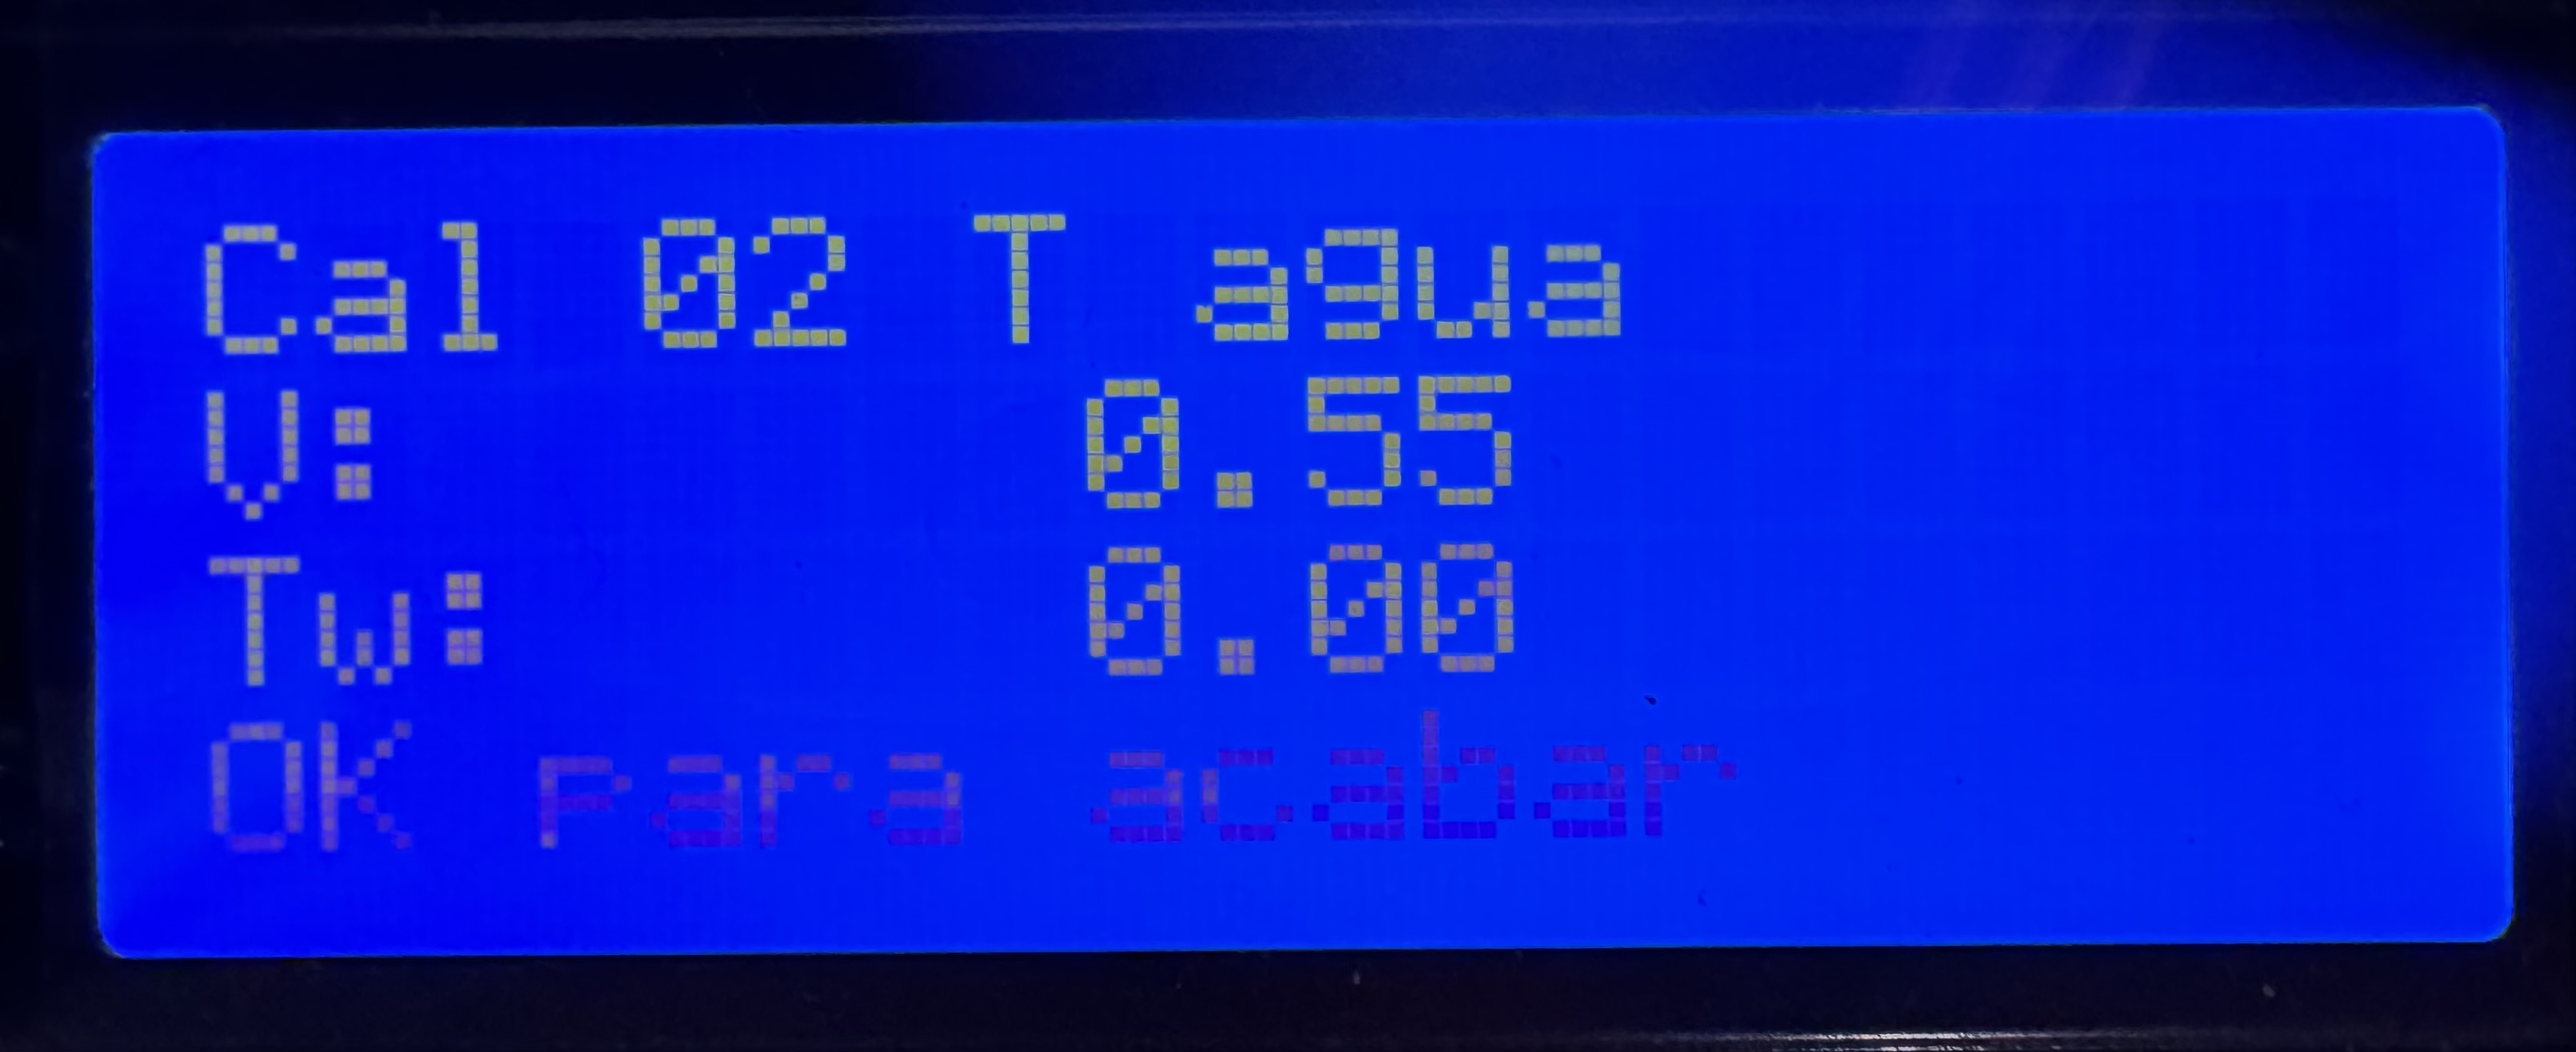
\psfig{file=Figuras/O2agua.jpeg,width=8cm,angle=0}} 
\caption{$2^{\circ}$ procedimiento para la calibración del sensor de concentración de $O_2$}\label{patalla:O2agua} 
\end{figure}

\begin{itemize}
\item Línea 1: \textbf{Cal 02 T aire}.
\item Línea 2: \textbf{V:} es la tensión que está leyendo el sensor.
\item Línea 3: \textbf{Ta:} El valor de la temperatura del agua proporcionado por el sensor DS18B20 (no es el sensor de conductividad).
\item Línea 4: \textbf{OK para acabar}. Una vez que este todo pulsamos OK para acabar.
\end{itemize}

\item Para este procedimiento necesitamos un un baso de agua en el que introducimos una bomba de oxigeno de un acuario. Tenemos que dejar la bomba encendida durante 10 min con objeto de saturar el agua de $O_2$. Una vez hecho esto introducimos la sonda de concentración de $O_2$ y el sensor DS18B20 y esperamos 1 minuto a que al tensión se estabilice. Una vez hecho esto pulsamos OK.

En el archivo \emph{config.txt} se actualizaran los valores \emph{CAL1\_V} y \emph{CAL1\_T}.
\end{enumerate}


\begin{tcolorbox}
[colback=red!5!white,colframe=red!75!black,fonttitle=\bfseries,title=VIDA DEL SENSOR $O_2$]

Según el fabricante la cabeza de la probeta hay que cambiarla cada 4 o 5 meses en caso de agua limpia. La vida de la probeta es de 1 año.

Para ver el procedimiento para cambiar la cabeza de la probeta se puede ver en los link provistos al comienzo de esta sección

\end{tcolorbox}

%%%%%%%%%%%%%%%%%%%%%%%%%%%%%%%%%%%%%%%%%%%%%%%%%%%%%%%%%%%%%%%%%%%%%%%%%%%%%%%%%%%%%%%%%%%%%%%%%%%%%%
\newpage

\section{Sensor de conductividad y calibración}

La conductividad es el recíproco de la resistividad de un objeto. Representa la capacidad de un material para conducir una corriente. En un líquido, la conductividad es una medida de la capacidad de una solución para conducir electricidad y puede reflejar la cantidad de sustancias disueltas o la salinidad de una fuente de agua, por lo que es un parámetro importante en la monitorización de la calidad del agua.

El sensor de conductividad eléctrica analógico Gravity PRO de DFRobot (K=1) SEN0451 está especialmente diseñado para medir la conductividad en soluciones acuosas y así evaluar la calidad del agua. Estos sensores de conductividad se utilizan a menudo en hidroponía, acuicultura, detección ambiental del agua y otros campos.

Como versión mejorada del medidor de conductividad eléctrica analógico, esta versión pro ha mejorado considerablemente la durabilidad de la sonda, lo que permite su uso en la monitorización de la conductividad las 24 horas del día, los 7 días de la semana. Además, el termómetro de resistencia de platino integrado PT1000 facilita la medición de datos de temperatura compensada.

\begin{verbatim}
https://www.dfrobot.com/product-2565.html
https://wiki.dfrobot.com/SKU_SEN0451_Gravity_Analog_Electrical_Conductivity_Sensor_PRO_K_1
\end{verbatim}

La medida de la conductividad es fuertemente dependiente de la temperatura es por eso que la sonda de conductividad viene con una sonda de temperatura incorporada. La sonda de conductividad viene caracterizada por un único parámetro K (ganancia) cuyo valor inicial viene medido de fábrica y que se puede encontrar en el cable de la sonda.

En caso que necesite recalibrar la sonda el procedimiento es sencillo:

Una vez estamos en la pantalla principal pulsamos el botón MODE 5 veces\footnote{Si se pasa la pantalla, siga pulsando hasta que vuelva la pantalla principal} hasta que sale la pantalla (figura \ref{patalla:EC}). Fíjese que es la parte superior aparece la frase: \textbf{Calc EC}.

\begin{figure}[htbp!] 
\centering{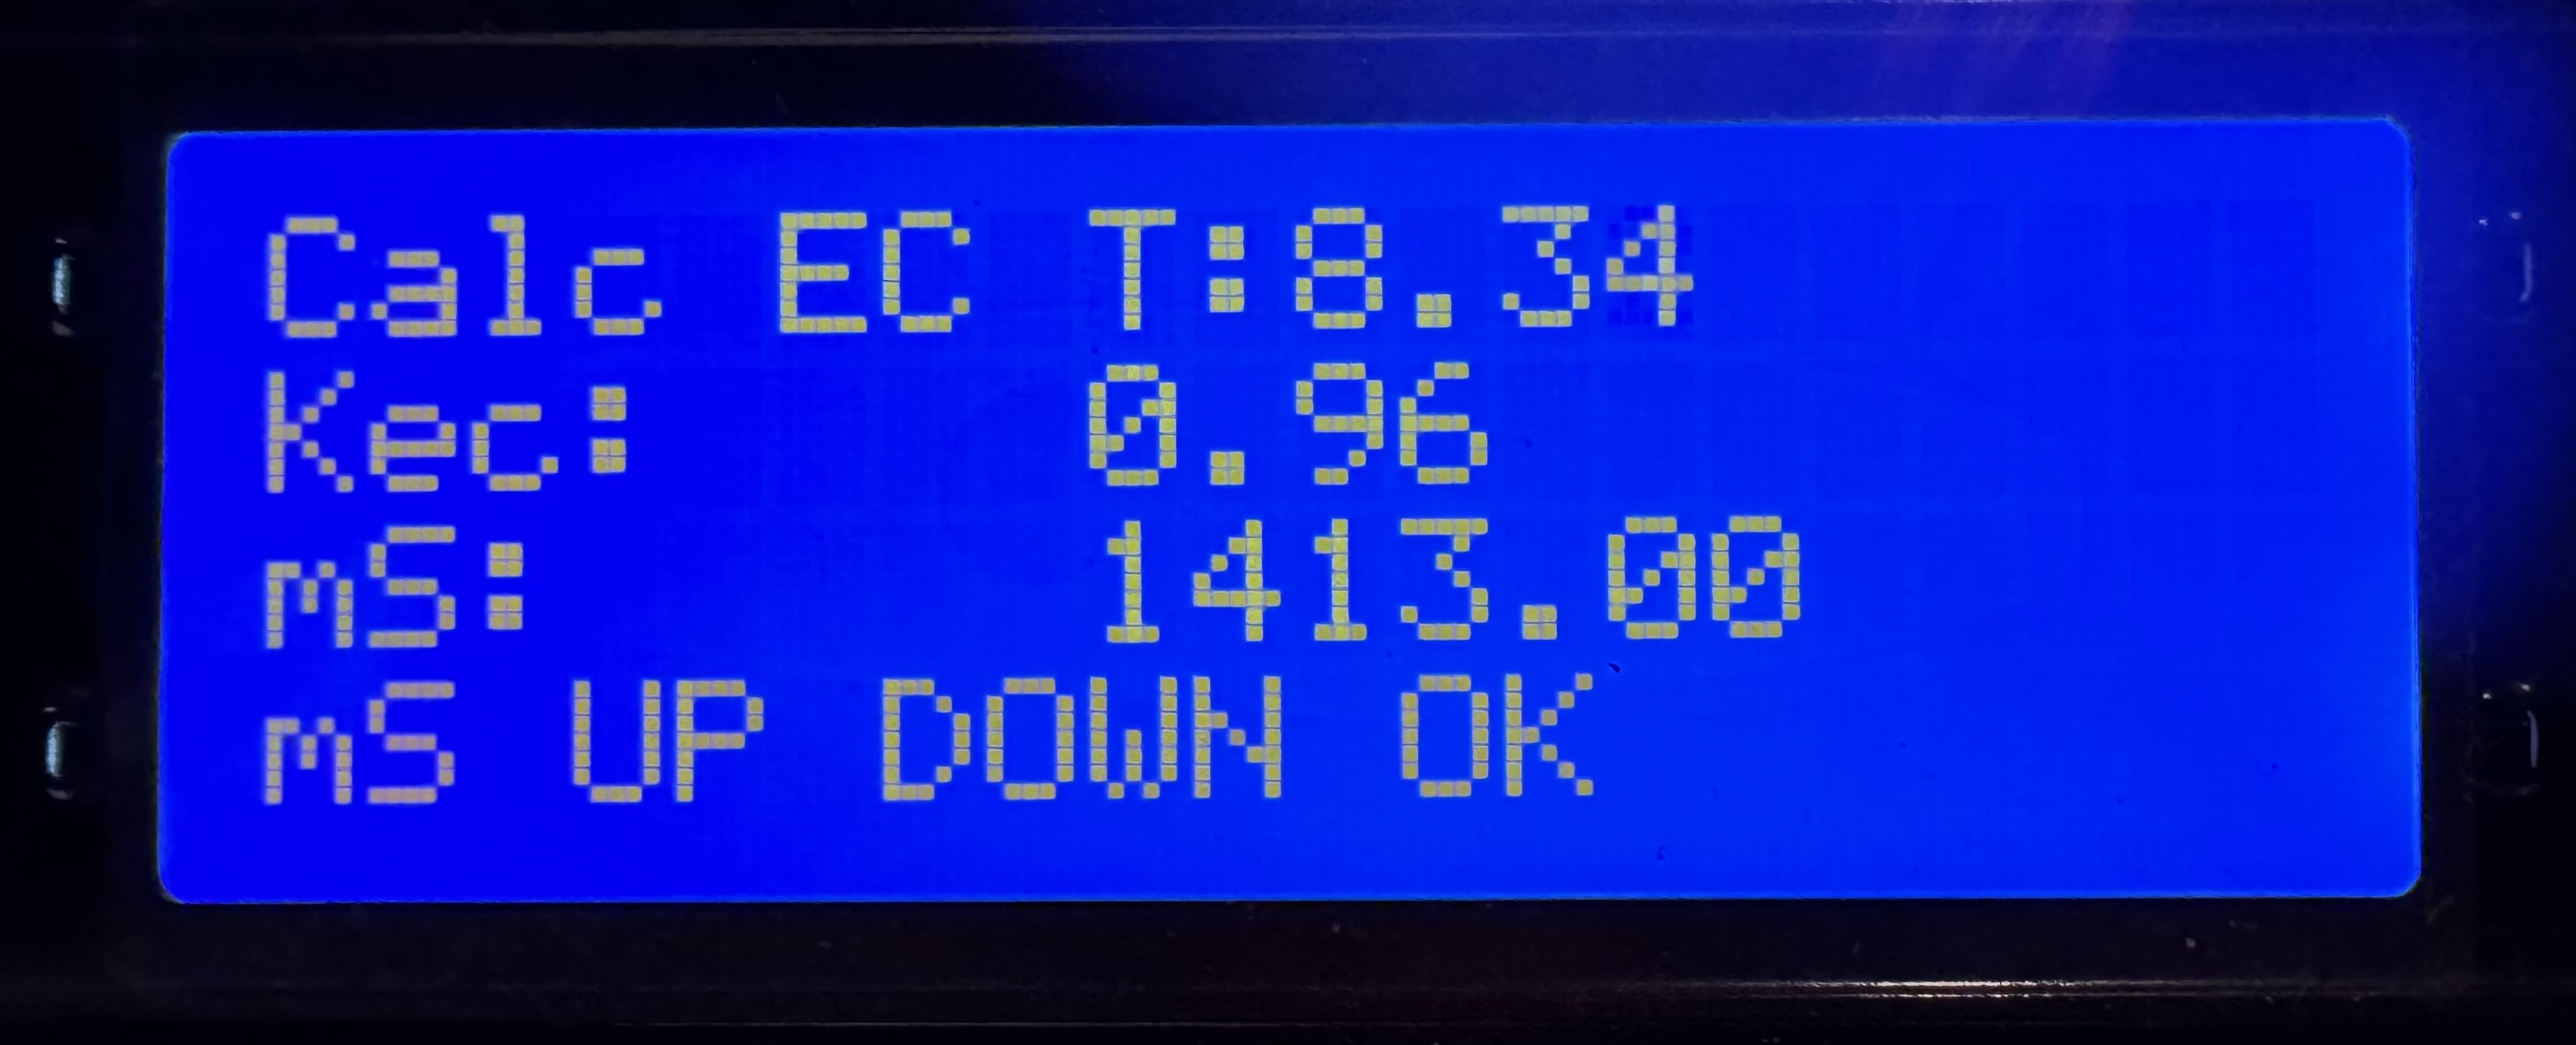
\psfig{file=Figuras/ECcal.jpeg,width=8cm,angle=0}} 
\caption{Procedimiento para la calibración del sensor de conductividad}\label{patalla:EC} 
\end{figure}

\begin{itemize}
\item Línea 1: \textbf{Calc EC} y la temperatura que está leyendo la sonda en ese instante.
\item Línea 2: \textbf{Kec:} es el valor actual de ganancia de la sonda de conductividad.
\item Línea 3: \textbf{mS:} Es el valor de la conductividad de la solución que se usa para calibrar.
\item Línea 4: \textbf{mS UP DOWN OK}. Podemos variar el valor de conductividad de la solución de calibración con UP o DOWN y una vez que este todo pulsamos OK para acabar.
\end{itemize}

El procedimiento es el siguiente: Metemos la probeta del conductividad, previa limpieza, en un líquido de conductividad conocida y \underline{esperamos un minuto} a que se estabilice la tensión. Mientras vamos ajustando el campo mS con UP y DOWN y pulsamos OK.

En el archivo \emph{config.txt} se actualizaran los valores \emph{Kec}, \emph{mS} y \emph{Tec}.

\begin{tcolorbox}
[colback=red!5!white,colframe=red!75!black,fonttitle=\bfseries,title=VIDA DEL SENSOR DE CONDUCTIVIDAD]

El fabricante no da ningún dato ni de cuanto tiempo tiene que pasar entre recalibraciones ni de cuanto es la vida de la probeta por lo que hay que ir haciendo medidas periódicas con otra sonda y comparar.

La probeta que tenemos en el equipo de prueba lleva instalada 3-4 meses y sigue funcionando bien.

\end{tcolorbox}
\clearpage

\chapter{Configurando el IDE de Arduino.}

%\begin{figure}[htbp!]
%\centering{\psfig{file=Figuras/circuito.png,width=14cm,angle=0}}
%\caption{Circuito de la competici\'{o}n}
%\end{figure}


%\begin{tcolorbox}
%[colback=red!5!white,colframe=red!75!black,fonttitle=\bfseries,title=NO OLVIDAR:]
%Instalar el driver CH340\footnote{Disponible en EV} para poder usar el Arduino no original e instalar la librer\'{\i}a \emph{TimerOne}.
%\end{tcolorbox}

\section{Introducción}

Para ser capaces de instalar futuras versiones del Software lo primero que tenemos que hacer es configurar de forma correcta el IDE de Arduino para que pueda trabajar con el micro que se ha usado para el equipo. 
\begin{itemize}
\item El IDE de Arduino es el programa que se usa para programar los micros. Se ha usado este programa por su simplicidad.
\item La placa que se usa es una Fire-Beetle, que a su vez se basa en un micro esp32. Este micro tiene capacidad de comunicación Wifi y Bluetooth, y potencia suficiente para ejecutar todas las funcionalidades de este equipo.
\end{itemize}

\section{Preparando el IDE de Arduino para trabajar con el esp32}

\begin{enumerate}
\item Abrimos el IDE de Arduino.
\item En la pestaña que pone Arduino (arriba a la izquierda) seleccionamos preferencias.
\item Hay un campo para meter URL para buscar nuevas placas, En ese campo copiamos lo siguiente:
\begin{verbatim}
https://raw.githubusercontent.com/espressif/arduino-esp32/gh-pages
/package_esp32_index.json
\end{verbatim}
\item Vamos ahora a: herramientas $\rightarrow$ placas $\rightarrow$ gestor de tarjetas. En el buscador ponemos $esp32$
\item instalamos:\emph{esp32 by Espressif Systems}
\item Ya podemos seleccionar la placa \textbf{FireBeetle-ESP32} en el menú de placas. Hay muchísimas placas que montan el esp32\footnote{En el comienzo del programa vienen estas instrucciones.}.
\end{enumerate}

\section{Instalar las librerías}

Para instalar las librerías proceda de la siguiente manera:

\begin{enumerate}
\item Una vez instalada la última versión del IDE y haber configurado el repositorio de placas de Espressiv (esp32). Abrimos la versión del programa proporcionada que ha de llamarse \emph{Acuacol\_definitivoVX.ino} (donde X es un número). Habrá muchos más ficheros \emph{.ino} pero este es el que gestiona todos los demás (debe coincidir con el nombre de la carpeta que contiene todos los ficheros .ino).
\item En las pestañas de arriba de la ventana seleccionamos Sketch $\rightarrow$ Include Library $\rightarrow$ Manage Libraries. Se abrirá a la izquierda un menú para instalar librerías.
\item Arriba a la izquierda sale una ventana de búsqueda, vamos buscando las librerías y las instalamos. No instalaremos \emph{wire}, porque ya está instalada.
\end{enumerate}

\section{Librerías a instalar para ejecutar el programa:}
Son las librerías que vienen en los \emph{include} al comienzo del programa.
\begin{enumerate}
\item \emph{Wire}. Debe estar ya instalada.
\item \emph{RTClib} Librería para el manejo del reloj RTC. De Adafruit. Instalar con dependencias.
\item \emph{OneWire} Librería para los sensores DS18B20. De Jim Studt...
\item \emph{DallasTemperature} Librería para los sensores DS18B20. De Miles Burton V3.9.0. Instalar con dependencias.
\item \emph{SPI} Librería para la lectura de la tarjeta microSD. Ya instalada
\item \emph{SD} Librería para la lectura de la tarjeta microSD. Se instala cuando instalas el esp32.
\item \emph{DHT sensor library} Librería para sensores ambientales DHT22. De Adrafruit. Instalar con dependencias.
\item \emph{WiFi} Librería para comunicación WIFI. Instalada.
\item \emph{time} Librería para el manejo del tiempo (seguramente la instala RTCLib). 
\item \emph{PubSubClient} Librería para comunicación MQTT. De Nick O'Leary. 
\item \emph{ArduinoJson} Librería para mandar y recibir datos Json. De Benoit Blanchon
\item \emph{TCA9555} Librería para trabajar con el modulo de expasión de entradas y salidas digitales I2C TCA9555
\item \emph{Adafruit\_ADS1X15} Librería para trabajar con el convertidor de entradas analógicas ADC115. Instalar con dependencias.
\item \emph{LiquidCrystal\_I2C} Librería para el manejo de la pantalla lcd I2C. De Frank Brabander. Da un warning al compilar, avisa que la librería no esta diseñada para la arquitectura del Fire-Beetle. Aún así funciona.
\end{enumerate}

Solo nos queda comprobar que todas las librerías están bien instaladas dándole al botón de compilar. La primera vez tarda mucho, luego ya va más rápido. Si todo sale de forma correcta puede cargar el programa en el Fire-Beetle.

\begin{tcolorbox}
[colback=red!5!white,colframe=red!75!black,fonttitle=\bfseries,title=DFRobot FireBeetle-esp32 V4.0 ]
Para probar el programa en la placa DFRobot FireBettle ESP32. En el menú herramientas:
\begin{enumerate}
\item Seleccionamos FireBeetle-esp32, en el menú de placas
\item Upload speed: 115200 (Cambiar por defecto viene 921600)
\item Seleccionamos el puerto. Debe ser el puerto que aparezca nuevo al conectar Fire Beetle.
\item Le damos a la flecha que hay arriba a la izquierda, para cargar el programa.
\end{enumerate}
\end{tcolorbox}

Una vez cargado el sistema se iniciará automáticamente.











\clearpage



%\include{Cap3_MPCT}
%\clearpage

%\include{Cap4_OFFCAN}
%\clearpage

%\include{Cap5_RMPC}
%\clearpage

\end{document}





